\documentclass[11pt]{book}

% ---------- Packages ----------
\usepackage[utf8]{inputenc}
\usepackage[T1]{fontenc}
\usepackage{amsmath, amssymb, amsthm}
\usepackage{mathtools}
\usepackage{geometry}
\usepackage{graphicx}
\usepackage{tikz}
\usepackage{xcolor}
\usepackage{enumitem}
\usepackage{hyperref}
\usepackage{listings}
\usepackage{fancyhdr}
\usepackage{tcolorbox}
\tcbuselibrary{theorems}
\usepackage{booktabs}
\usepackage{array}

\geometry{margin=1in}

% ---------- Colors ----------
\definecolor{frameblue}{RGB}{20,60,120}
\definecolor{framegray}{RGB}{245,245,245}
\definecolor{codebg}{RGB}{248,248,248}
\definecolor{examplegreen}{RGB}{20,90,50}
\definecolor{reviewred}{RGB}{140,20,20}

% ---------- Header/Footer ----------
\pagestyle{fancy}
\fancyhf{}
\fancyhead[L]{\small\textit{Finite Frame Theory}}

\fancyfoot[C]{\thepage}
\renewcommand{\headrulewidth}{0.4pt}

% ---------- Theorem environments ----------
\theoremstyle{plain}
\newtheorem{theorem}{Theorem}[section]
\newtheorem{proposition}[theorem]{Proposition}
\newtheorem{lemma}[theorem]{Lemma}
\newtheorem{corollary}[theorem]{Corollary}

\theoremstyle{definition}
\newtheorem{definition}[theorem]{Definition}

\theoremstyle{remark}
\newtheorem{remark}[theorem]{Remark}
\newtheorem*{remark*}{Remark}

% ---------- Custom boxes ----------
\newtcolorbox{keyidea}[1][]{
	colback=framegray,
	colframe=frameblue,
	boxrule=0.8pt,
	arc=2pt,
	left=8pt, right=8pt, top=6pt, bottom=6pt,
	title={\textbf{Key Idea}},
	fonttitle=\bfseries\color{white},
	coltitle=white,
	colbacktitle=frameblue,
	#1
}

\newtcolorbox{examplebox}[1][]{
	colback=white,
	colframe=examplegreen,
	boxrule=0.8pt,
	arc=2pt,
	left=8pt, right=8pt, top=6pt, bottom=6pt,
	#1
}

\newtcolorbox{exercisebox}[1][]{
	colback=white,
	colframe=black!60,
	boxrule=0.6pt,
	arc=1pt,
	left=8pt, right=8pt, top=6pt, bottom=6pt,
	#1
}
\newtcolorbox{reviewbox}[1][]{
	colback=red!3,
	colframe=reviewred,
	boxrule=0.8pt,
	arc=2pt,
	left=8pt, right=8pt, top=6pt, bottom=6pt,
	title={\textbf{Exam Tip}},
	fonttitle=\bfseries\color{white},
	coltitle=white,
	colbacktitle=reviewred,
	#1
}
% ---------- Code listing style ----------
\lstdefinestyle{pythonstyle}{
	backgroundcolor=\color{codebg},
	basicstyle=\ttfamily\small,
	keywordstyle=\color{blue!70!black}\bfseries,
	commentstyle=\color{green!40!black}\itshape,
	stringstyle=\color{orange!70!black},
	numbers=left,
	numberstyle=\tiny\color{gray},
	stepnumber=1,
	numbersep=8pt,
	frame=single,
	rulecolor=\color{gray!40},
	breaklines=true,
	showstringspaces=false,
	language=Python,
	tabsize=4,
}
\lstset{style=pythonstyle}

% ---------- Custom commands ----------
\newcommand{\R}{\mathbb{R}}
\newcommand{\C}{\mathbb{C}}
\newcommand{\N}{\mathbb{N}}
\newcommand{\F}{\mathbb{F}} % field, R or C
\newcommand{\norm}[1]{\left\| #1 \right\|}
\newcommand{\inner}[2]{\left\langle #1, #2 \right\rangle}
\newcommand{\setdef}[2]{\left\{ #1 \;:\; #2 \right\}}
\newcommand{\spn}{\operatorname{span}}
\newcommand{\rank}{\operatorname{rank}}
\newcommand{\tr}{\operatorname{tr}}
\newcommand{\Real}{\operatorname{Re}}
\newcommand{\Imag}{\operatorname{Im}}
\newcommand{\FP}{\operatorname{FP}}
\newcommand{\Gr}{\operatorname{Gr}}
\newcommand{\Z}{\mathbb{Z}}
\newcommand{\E}{\mathbb{E}}
\newcommand{\minimize}{\operatorname*{minimize}}
\newcommand{\argmin}{\operatorname*{argmin}}

\newlist{theoexercises}{enumerate}{1}
\setlist[theoexercises]{label=\textbf{T\arabic*.}, itemsep=5pt, topsep=4pt, leftmargin=1.8em}
\newlist{compexercises}{enumerate}{1}
\setlist[compexercises]{label=\textbf{C\arabic*.}, itemsep=5pt, topsep=4pt, leftmargin=1.8em}


\title{\textbf{Finite Frame Theory:\\Geometry and Computation}}
\author{Lecture Notes}
\date{}

\begin{document}
	
	\begin{titlepage}
		\centering
		\vspace*{2cm}
		{\Huge \textbf{Finite Frame Theory}}\\[0.5cm]
		{\Large Geometry and Computation}\\[2cm]
		{\LARGE \textbf{Hussein Mastaneh}}\\[0.3cm]
		{\Large Persian Gulf University of Bushehr}\\[1cm]
		{\large h.mastaneh@gmail.com}\\[3cm]
		{\large Lecture Notes}\\[1cm]
		\vfill
		{\large \today}
	\end{titlepage}
	
	\tableofcontents
	\newpage

%%%%%%%%%%%%%%%%%%%Chapters%%%%%%%%%%%
\chapter{Motivation and Foundations}
\label{ch:motivation}
\fancyhead[R]{\small\textit{Chapter 1: Motivation and Foundations}}
\section{Why Study Frames? Redundancy as a Feature}
\label{sec:why-frames}

Almost every linear algebra course you have taken builds toward the same destination: a \emph{basis}. A basis of a vector space $V$ is a set of vectors that is simultaneously \emph{spanning} (every vector in $V$ can be written as a combination of them) and \emph{linearly independent} (no vector in the set is redundant --- each one is doing essential work). This is an elegant and economical idea. If $\dim V = n$, a basis has exactly $n$ vectors: no more, no fewer.

This chapter begins by asking you to set that economy aside, at least temporarily, and consider a different question.

\begin{quote}
\itshape What if we deliberately use \emph{more} vectors than the dimension of the space requires?
\end{quote}

At first this sounds wasteful. If $n$ vectors already span $\R^n$, why would anyone use $m > n$ vectors to do the same job? The answer, which is the entire motivation for this course, is that redundancy is not always waste --- it can be a resource. A redundant representation of a vector can be:

\begin{itemize}
  \item \textbf{Robust to noise.} If you measure a vector's coordinates with respect to a basis and one measurement is corrupted, you have lost information that cannot be recovered from the others. If you have redundant measurements, the corrupted one can sometimes be detected, discarded, or corrected using the rest.
  \item \textbf{Robust to erasure.} In communication and signal processing, data is sometimes lost entirely in transmission (an ``erasure''). A redundant representation can often be perfectly reconstructed even when some of its pieces never arrive.
  \item \textbf{Flexible.} A basis gives you exactly one way to write each vector as a combination of the basis elements. A redundant spanning set gives you a whole family of ways, and you are free to choose the representation best suited to your purposes (smallest coefficients, sparsest representation, most numerically stable, and so on).
  \item \textbf{Symmetric.} Certain highly redundant, highly symmetric configurations of vectors (we will meet our first examples by the end of this chapter) treat every direction in space with perfect uniformity, in a sense we will make precise. No basis can do this --- the asymmetry of having exactly $n$ vectors in an $n$-dimensional space forces some directions to be treated differently from others.
\end{itemize}

\textbf{Frame theory} is the mathematical framework for making these ideas precise. A \emph{frame} is, roughly speaking, a spanning set of vectors --- typically with redundancy, i.e., more vectors than the dimension requires --- equipped with quantitative control over how that redundancy behaves. The formal definition is the subject of Chapter 2 (next week's notes); this week, we build the geometric intuition and the linear algebra toolkit that the definition will rest on.

\begin{keyidea}
A frame is a generalization of a basis that permits (and often deliberately uses) redundancy. The price of redundancy is that representations are no longer unique. The payoff is robustness, flexibility, and --- as we will soon see geometrically --- a kind of balance that no basis can achieve.
\end{keyidea}

\subsection{A First Picture}
\label{subsec:first-picture}

Consider the plane $\R^2$. A basis consists of exactly two linearly independent vectors. The standard basis $\{e_1, e_2\}$, with $e_1 = (1,0)$ and $e_2 = (0,1)$, is the most familiar example: it is orthonormal, meaning each vector has length $1$ and the two vectors are perpendicular.

Now consider three vectors in $\R^2$ pointing toward the vertices of an equilateral triangle centered at the origin:
$$
f_1 = (1, 0), \qquad f_2 = \left(-\tfrac{1}{2}, \tfrac{\sqrt 3}{2}\right), \qquad f_3 = \left(-\tfrac{1}{2}, -\tfrac{\sqrt 3}{2}\right).
$$
These three vectors are linearly \emph{dependent} (any two of them already span $\R^2$, so the third is redundant; indeed $f_1+f_2+f_3=0$), but they still span $\R^2$, and they do so with a kind of $120^\circ$-rotational symmetry that no pair of vectors can replicate. We will see by the end of this chapter, and prove rigorously in Chapter 4, that this triangular configuration is an example of a \emph{tight frame}: a redundant spanning set that distributes ``energy'' perfectly evenly across every direction in the plane. Figure \ref{fig:basis-vs-frame} previews the visual difference between the two configurations.

\begin{figure}[h]
\centering
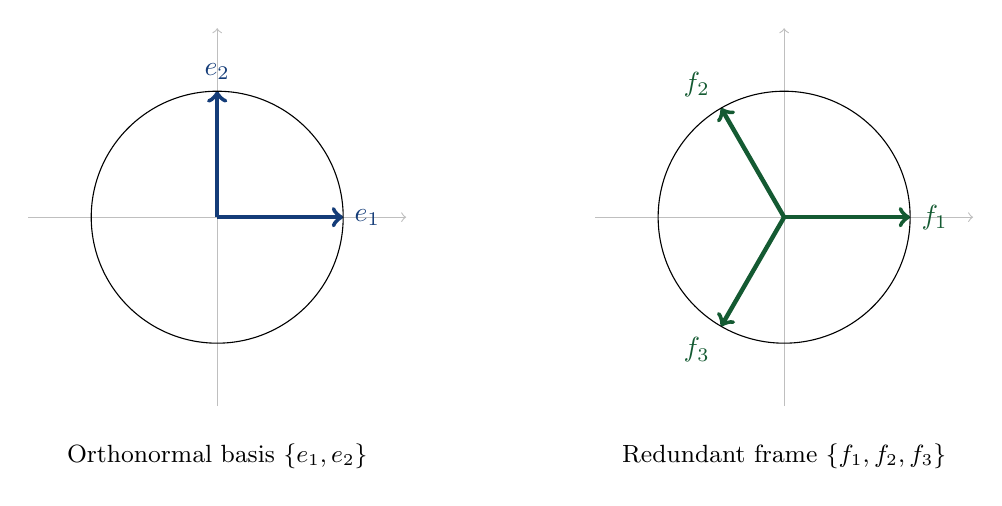
\begin{tikzpicture}[scale=1.6]
  % Left: orthonormal basis
  \begin{scope}
    \draw[->, gray!50, thin] (-1.5,0) -- (1.5,0);
    \draw[->, gray!50, thin] (0,-1.5) -- (0,1.5);
    \draw[->, frameblue, ultra thick] (0,0) -- (1,0) node[right] {$e_1$};
    \draw[->, frameblue, ultra thick] (0,0) -- (0,1) node[above] {$e_2$};
    \draw (0,0) circle (1);
    \node at (0,-1.9) {\small Orthonormal basis $\{e_1, e_2\}$};
  \end{scope}
  % Right: triangular frame
  \begin{scope}[xshift=4.5cm]
    \draw[->, gray!50, thin] (-1.5,0) -- (1.5,0);
    \draw[->, gray!50, thin] (0,-1.5) -- (0,1.5);
    \draw[->, examplegreen, ultra thick] (0,0) -- (1,0) node[right] {$f_1$};
    \draw[->, examplegreen, ultra thick] (0,0) -- (-0.5,0.866) node[above left] {$f_2$};
    \draw[->, examplegreen, ultra thick] (0,0) -- (-0.5,-0.866) node[below left] {$f_3$};
    \draw (0,0) circle (1);
    \node at (0,-1.9) {\small Redundant frame $\{f_1, f_2, f_3\}$};
  \end{scope}
\end{tikzpicture}
\caption{An orthonormal basis (left) versus a redundant, symmetric spanning set (right) in $\R^2$. Both span the plane. The right-hand configuration has three-fold rotational symmetry that two vectors alone cannot achieve.}
\label{fig:basis-vs-frame}
\end{figure}

This picture is the geometric heart of the course, and we will return to it constantly. For now, simply notice: \emph{both} pictures span $\R^2$, but they are doing geometrically different things, and the difference is something we will learn to measure precisely.

\subsection{Where Frames Show Up}
\label{subsec:applications-preview}

To motivate the abstract definitions to come, here is a brief, non-exhaustive preview of where redundant spanning sets are useful in practice. We will revisit several of these applications in detail later in the course (particularly Weeks 10 and 11).

\begin{itemize}
  \item \textbf{Signal and image processing.} Redundant systems of vectors (generalizing wavelets and Fourier bases) are used to represent signals in ways that are robust to quantization error and compression artifacts.
  \item \textbf{Communications and coding theory.} When data is transmitted over a noisy or unreliable channel, redundant encodings allow the receiver to reconstruct the original message even if some pieces are lost (erasures) or corrupted (noise).
  \item \textbf{Compressed sensing.} Modern signal acquisition techniques exploit redundant, highly incoherent systems of vectors to recover high-dimensional signals from surprisingly few measurements.
  \item \textbf{Quantum information theory.} Certain highly symmetric finite frames (equiangular tight frames, in particular) are intimately connected to optimal quantum measurements.
\end{itemize}

You do not need to know anything about these fields to take this course. They are mentioned here only so that, as we develop the theory, you have a sense of why anyone bothered to develop it.

\section{Linear Algebra Review}
\label{sec:linalg-review}

Frame theory is built on a small number of linear algebra concepts, used repeatedly and combined in new ways. This section reviews exactly the material we need: inner product spaces, orthonormal bases, and spanning sets/linear independence, with an eye toward the question that will occupy us for the rest of the course: \emph{what happens when a spanning set has more vectors than the dimension of the space?}

Throughout, $\F$ denotes either $\R$ or $\C$; we work in the finite-dimensional space $\F^n$. The vast majority of examples in this course will use $\R^n$, especially in low dimensions where pictures are possible, but the complex case $\C^n$ is equally important in applications (especially quantum information theory and signal processing with complex exponentials) and the theory transfers with only minor modifications, which we flag as they arise.

\subsection{Inner Product Spaces}
\label{subsec:inner-product}

\begin{definition}[Inner product]
\label{def:inner-product}
Let $V$ be a vector space over $\F$. An \emph{inner product} on $V$ is a function $\inner{\cdot}{\cdot} : V \times V \to \F$ satisfying, for all $x, y, z \in V$ and $\alpha \in \F$:
\begin{enumerate}[label=(\roman*)]
  \item \textbf{Conjugate symmetry:} $\inner{x}{y} = \overline{\inner{y}{x}}$.
  \item \textbf{Linearity in the first argument:} $\inner{\alpha x + y}{z} = \alpha \inner{x}{z} + \inner{y}{z}$.
  \item \textbf{Positive definiteness:} $\inner{x}{x} \geq 0$, with equality if and only if $x = 0$.
\end{enumerate}
\end{definition}

\begin{remark*}
When $\F = \R$, conjugate symmetry is simply symmetry: $\inner{x}{y} = \inner{y}{x}$. The standard inner product on $\R^n$ is the familiar dot product, $\inner{x}{y} = \sum_{k=1}^n x_k y_k$. On $\C^n$, the standard inner product is $\inner{x}{y} = \sum_{k=1}^n x_k \overline{y_k}$, where the conjugate on the second argument is exactly what is needed to make positive definiteness hold: $\inner{x}{x} = \sum_k |x_k|^2 \geq 0$.

\emph{Convention check.} Some texts place the conjugate on the first argument instead of the second; this is purely a convention and has no mathematical consequence as long as it is used consistently. We will consistently conjugate the second argument, matching the most common convention in the signal processing and frame theory literature (and matching NumPy's \texttt{vdot} function, which we will use in the lab).
\end{remark*}

The inner product immediately gives us a notion of length:

\begin{definition}[Norm]
\label{def:norm}
The \emph{norm} (or \emph{length}) induced by an inner product is
$$
\norm{x} := \sqrt{\inner{x}{x}}.
$$
\end{definition}

The norm satisfies the triangle inequality $\norm{x+y} \le \norm{x} + \norm{y}$ and the homogeneity property $\norm{\alpha x} = |\alpha| \, \norm{x}$, both of which you likely proved in your linear algebra course using the following essential inequality.

\begin{theorem}[Cauchy--Schwarz Inequality]
\label{thm:cauchy-schwarz}
For all $x, y \in V$,
$$
\left| \inner{x}{y} \right| \leq \norm{x} \, \norm{y},
$$
with equality if and only if $x$ and $y$ are linearly dependent (i.e., one is a scalar multiple of the other).
\end{theorem}

We state this without proof, as it is a standard result you should have already seen; if it is unfamiliar, any linear algebra textbook will supply a proof, and it is a worthwhile exercise to reconstruct.

\begin{remark*}
Cauchy--Schwarz will be the single most frequently invoked inequality in this entire course. The quantity $|\inner{x}{y}|$ measures, in a precise sense, how much $x$ and $y$ ``overlap'' or ``align,'' and Cauchy--Schwarz says this overlap can never exceed the product of their lengths. When we define frame bounds in Chapter 2, the quantity $\sum_i |\inner{x}{f_i}|^2$ --- a sum of squared overlaps between $x$ and each frame vector $f_i$ --- is the central object of study, and intuition for it is built entirely on intuition for $|\inner{x}{y}|$ itself.
\end{remark*}

\begin{definition}[Orthogonality]
\label{def:orthogonal}
Two vectors $x, y \in V$ are \emph{orthogonal} if $\inner{x}{y} = 0$. A set of vectors $\{v_1, \dots, v_k\}$ is \emph{orthogonal} if $\inner{v_i}{v_j} = 0$ for all $i \neq j$, and \emph{orthonormal} if it is orthogonal and, additionally, $\norm{v_i} = 1$ for every $i$.
\end{definition}

\subsection{Spanning Sets, Linear Independence, and Bases}
\label{subsec:spanning-bases}

\begin{definition}[Span]
\label{def:span}
Given vectors $v_1, \dots, v_m \in V$, their \emph{span} is the set of all linear combinations:
$$
\spn\{v_1, \dots, v_m\} := \setdef{\sum_{i=1}^m c_i v_i}{c_1, \dots, c_m \in \F}.
$$
If $\spn\{v_1, \dots, v_m\} = V$, we say the set $\{v_1, \dots, v_m\}$ \emph{spans} $V$, or is a \emph{spanning set} for $V$.
\end{definition}

\begin{definition}[Linear independence]
\label{def:linear-independence}
Vectors $v_1, \dots, v_m \in V$ are \emph{linearly independent} if the only solution to
$$
c_1 v_1 + c_2 v_2 + \cdots + c_m v_m = 0
$$
is $c_1 = c_2 = \cdots = c_m = 0$. If a nontrivial solution exists, the vectors are \emph{linearly dependent}.
\end{definition}

\begin{definition}[Basis]
\label{def:basis}
A set $\{v_1, \dots, v_n\} \subset V$ is a \emph{basis} for $V$ if it is both a spanning set and linearly independent.
\end{definition}

A fundamental fact, which you should have proven in your first linear algebra course, is that \emph{every basis of a finite-dimensional vector space $V$ has the same number of elements}; this common number is the \emph{dimension} of $V$, denoted $\dim V$. We will take $\dim V = n$ throughout, working in $V = \F^n$.

Here is the observation that frame theory is built on, stated as a proposition so that we can refer back to it precisely.

\begin{proposition}[Redundant spanning sets exist]
\label{prop:redundant-spanning}
Let $V$ be an $n$-dimensional vector space, and let $m > n$. Then there exist sets of $m$ vectors $\{v_1, \dots, v_m\} \subset V$ that span $V$. Any such set is necessarily linearly \emph{dependent}.
\end{proposition}

\begin{proof}
For existence: take any basis $\{e_1, \dots, e_n\}$ of $V$, and adjoin any $m - n$ additional vectors of $V$ (for instance, repeat $e_1$ a total of $m-n$ times, or pick arbitrary vectors). The resulting set of $m$ vectors still spans $V$, since it contains a spanning set as a subset.

For dependence: this is an immediate consequence of the fact (proved in any first linear algebra course, often called the Steinitz exchange lemma or a corollary of it) that no linearly independent set in an $n$-dimensional space can have more than $n$ elements. Since $m > n$, the set $\{v_1, \dots, v_m\}$ cannot be linearly independent.
\end{proof}

This proposition is almost trivial to prove, but its consequence is the entire subject of this course: \emph{whenever we use more vectors than the dimension requires, linear dependence is unavoidable, but this dependence can be harnessed rather than merely tolerated.} The redundant vectors are not ``wasted''; as we saw in Section \ref{subsec:first-picture}, they can be arranged to provide symmetry, robustness, and flexibility that no basis (with exactly $n$ vectors) could provide. Distinguishing a \emph{useful} redundant spanning set from an arbitrary, poorly-behaved one is precisely what the frame bounds $A$ and $B$ --- to be defined next week --- are designed to do.

\subsection{Orthonormal Bases and Coordinate Representations}
\label{subsec:onb}

Orthonormal bases deserve special attention because they make the relationship between a vector and its ``coordinates'' completely transparent, and this transparency is exactly what we will have to work to recover in the redundant setting.

\begin{theorem}[Orthonormal expansion]
\label{thm:onb-expansion}
Let $\{e_1, \dots, e_n\}$ be an orthonormal basis of $V$. Then every $x \in V$ can be written uniquely as
$$
x = \sum_{k=1}^n \inner{x}{e_k} \, e_k,
$$
and moreover,
$$
\norm{x}^2 = \sum_{k=1}^n \left| \inner{x}{e_k} \right|^2. \qquad \text{(Parseval's identity)}
$$
\end{theorem}

\begin{proof}
Since $\{e_1, \dots, e_n\}$ is a basis, we may write $x = \sum_k c_k e_k$ for some uniquely determined scalars $c_k$. Taking the inner product of both sides with $e_j$ and using orthonormality,
$$
\inner{x}{e_j} = \sum_{k=1}^n c_k \inner{e_k}{e_j} = c_j,
$$
since $\inner{e_k}{e_j} = 0$ for $k \neq j$ and $\inner{e_j}{e_j} = 1$. This proves $c_j = \inner{x}{e_j}$, giving the expansion formula. For Parseval's identity,
$$
\norm{x}^2 = \inner{x}{x} = \inner{\sum_k c_k e_k}{\sum_j c_j e_j} = \sum_{k,j} c_k \overline{c_j} \inner{e_k}{e_j} = \sum_{k=1}^n |c_k|^2 = \sum_{k=1}^n |\inner{x}{e_k}|^2,
$$
using orthonormality once more to collapse the double sum to a single sum.
\end{proof}

\begin{remark*}
This theorem is the single most important fact to internalize before next week, because the entire definition of a frame is obtained by asking: \emph{what happens if we drop the requirement that $\{e_1, \dots, e_n\}$ be a basis (i.e., we allow redundancy, $m > n$, and we no longer require orthonormality), and ask only that an inequality version of Parseval's identity still hold?} That single question is the seed from which the formal definition of a frame, next week's central topic, will grow:
$$
A \norm{x}^2 \;\leq\; \sum_{i=1}^m |\inner{x}{f_i}|^2 \;\leq\; B \norm{x}^2 \qquad \text{for all } x \in V,
$$
for constants $0 < A \leq B < \infty$ called the \emph{frame bounds}. When $\{f_i\}$ happens to be an orthonormal basis, Theorem \ref{thm:onb-expansion} shows $A = B = 1$ exactly, with equality (not just inequality) in the middle expression. Frames generalize this by relaxing equality to a two-sided bound, and relaxing exact orthonormality to mere redundancy-with-control.
\end{remark*}

\subsection{Why Redundant Sets Need Two Numbers, Not One}
\label{subsec:why-two-bounds}

It is worth pausing on a subtlety that will matter enormously starting next week. Given a redundant spanning set $\{f_1, \dots, f_m\}$ with $m > n$, the quantity
$$
\sum_{i=1}^m |\inner{x}{f_i}|^2
$$
is no longer equal to $\norm{x}^2$ for every $x$ (as it was for an orthonormal basis by Parseval's identity); it merely lies between two multiples of $\norm{x}^2$, and \emph{which} multiples depends on the direction of $x$. Geometrically: a redundant set of vectors might ``illuminate'' some directions in space more than others. The smallest amount of illumination, over all directions $x$, is (essentially) the lower frame bound $A$; the largest amount of illumination is the upper frame bound $B$. A set is called \emph{tight} exactly when $A = B$ --- when every direction is illuminated equally --- and Section \ref{subsec:first-picture}'s triangular configuration was an example (which we will verify rigorously, and numerically, very soon).

\begin{exercisebox}[title={Exercise 1.1}]
Let $f_1 = (1,0)$ and $f_2 = (0, 2)$ in $\R^2$ (note: \emph{not} orthonormal, since $\norm{f_2} = 2 \ne 1$). Compute $\sum_{i=1}^2 |\inner{x}{f_i}|^2$ for $x = (1,0)$ and again for $x = (0,1)$. Observe that the two values are different, despite $\norm{x}^2 = 1$ in both cases. What does this tell you about how $\{f_1, f_2\}$ treats different directions in the plane?
\end{exercisebox}

\begin{exercisebox}[title={Exercise 1.2}]
Prove the converse direction implicit in Theorem \ref{thm:onb-expansion}: if $\{e_1, \ldots, e_n\}$ is an orthonormal \emph{set} (not assumed to be a basis) and $\sum_{k=1}^n |\langle x, e_k\rangle|^2 = \|x\|^2$ for every $x \in V$, then $\{e_1, \ldots, e_n\}$ must in fact be a basis of $V$ (equivalently, $n = \dim V$). (Hint: argue by contradiction --- what would the inner product computation in the proof of Theorem \ref{thm:onb-expansion} look like if a basis vector were missing?)
\end{exercisebox}

\section{First Steps in Python}
\label{sec:python-onramp}

Numerical computation is a central theme of this course, not an afterthought: many of the most important properties of frames (the frame bounds, tightness, dual frames) are most easily understood by computing them. We use Python with the NumPy library throughout, because it makes vector and matrix computation immediate and because the syntax is close enough to mathematical notation to be readable at a glance.

If you have never written a line of code before, this section is for you. If you have programmed before (in any language), you can skim this section and proceed directly to the lab exercises in Section \ref{sec:lab}.

\subsection{Why Python and NumPy}
\label{subsec:why-python}

\textbf{Python} is a general-purpose programming language known for readable syntax. \textbf{NumPy} (Numerical Python) is a library --- a collection of pre-written code --- that adds fast, convenient array and matrix operations to Python. Without NumPy, representing a vector and computing an inner product would require writing your own loops; with NumPy, these become one-line operations that closely mirror mathematical notation. Every computational lab in this course will use NumPy as its foundation, and later weeks will add \texttt{SciPy} (for linear algebra routines like eigenvalue decompositions) and \texttt{Matplotlib} (for plotting).

\subsection{Vectors as Arrays}
\label{subsec:vectors-as-arrays}

In NumPy, a vector in $\R^n$ is represented as a one-dimensional array.

\begin{lstlisting}[caption={Creating and inspecting vectors}]
import numpy as np

# A vector in R^2
x = np.array([1.0, 0.0])
y = np.array([0.0, 1.0])

print(x)        # [1. 0.]
print(x.shape)  # (2,)  -- this is a 1D array of length 2
\end{lstlisting}

The \texttt{.shape} attribute tells you the dimensions of an array; for a vector in $\R^n$, it will be \texttt{(n,)}.

\subsection{Inner Products and Norms}
\label{subsec:inner-products-numpy}

The inner product of two real vectors is computed with \texttt{np.dot}, and the norm with \texttt{np.linalg.norm}.

\begin{lstlisting}[caption={Computing inner products and norms}]
import numpy as np

x = np.array([1.0, 2.0])
y = np.array([3.0, -1.0])

inner_xy = np.dot(x, y)          # <x, y> = 1*3 + 2*(-1) = 1
norm_x   = np.linalg.norm(x)     # sqrt(1^2 + 2^2) = sqrt(5)

print(f"<x, y> = {inner_xy}")
print(f"||x|| = {norm_x:.4f}")
\end{lstlisting}

\begin{remark*}
For \emph{complex} vectors, recall from Section \ref{subsec:inner-product} that our inner product convention conjugates the second argument: $\inner{x}{y} = \sum_k x_k \overline{y_k}$. The function \texttt{np.dot} does \emph{not} conjugate, so for complex vectors you should use \texttt{np.vdot(y, x)} or write \texttt{np.dot(x, np.conj(y))} explicitly. We will need this starting in later chapters when complex frames appear; for this week's exercises, real vectors suffice.
\end{remark*}

\subsection{Verifying Cauchy--Schwarz Numerically}
\label{subsec:verify-cs}

A nice first programming exercise is to numerically verify the Cauchy--Schwarz inequality (Theorem \ref{thm:cauchy-schwarz}) on a few examples, as a sanity check on both the mathematics and your NumPy syntax.

\begin{lstlisting}[caption={Checking Cauchy--Schwarz on random vectors}]
import numpy as np

np.random.seed(0)  # for reproducibility

for trial in range(5):
    x = np.random.randn(3)   # random vector in R^3
    y = np.random.randn(3)

    lhs = abs(np.dot(x, y))
    rhs = np.linalg.norm(x) * np.linalg.norm(y)

    print(f"Trial {trial}: |<x,y>| = {lhs:.4f}, "
          f"||x|| ||y|| = {rhs:.4f}, "
          f"inequality holds: {lhs <= rhs}")
\end{lstlisting}

Running this will print \texttt{True} for every trial (up to floating-point rounding, the inequality should never be violated). This kind of numerical sanity check --- verifying a theorem on random or specific examples --- is a habit we will use throughout the course, especially when working with frame bounds, where direct computation by hand becomes impractical for $m$ and $n$ larger than $2$ or $3$.

\subsection{Plotting Vectors in the Plane}
\label{subsec:plotting}

Visualizing vectors in $\R^2$ is one of the best ways to build geometric intuition, and we will do this constantly. Matplotlib's \texttt{quiver} function draws arrows from the origin.

\begin{lstlisting}[caption={Plotting the basis and the triangular frame from Figure 1.1}]
import numpy as np
import matplotlib.pyplot as plt

# Orthonormal basis
e1 = np.array([1.0, 0.0])
e2 = np.array([0.0, 1.0])

# Triangular frame (3 vectors, 120 degrees apart)
f1 = np.array([1.0, 0.0])
f2 = np.array([-0.5, np.sqrt(3)/2])
f3 = np.array([-0.5, -np.sqrt(3)/2])

fig, axes = plt.subplots(1, 2, figsize=(10, 5))

# Left subplot: orthonormal basis
ax = axes[0]
ax.quiver(0, 0, e1[0], e1[1], angles='xy', scale_units='xy',
          scale=1, color='steelblue', width=0.012)
ax.quiver(0, 0, e2[0], e2[1], angles='xy', scale_units='xy',
          scale=1, color='steelblue', width=0.012)
ax.set_xlim(-1.5, 1.5)
ax.set_ylim(-1.5, 1.5)
ax.set_aspect('equal')
ax.set_title('Orthonormal basis')
ax.grid(True, alpha=0.3)

# Right subplot: triangular frame
ax = axes[1]
for f in [f1, f2, f3]:
    ax.quiver(0, 0, f[0], f[1], angles='xy', scale_units='xy',
              scale=1, color='seagreen', width=0.012)
ax.set_xlim(-1.5, 1.5)
ax.set_ylim(-1.5, 1.5)
ax.set_aspect('equal')
ax.set_title('Redundant, symmetric frame')
ax.grid(True, alpha=0.3)

plt.tight_layout()
plt.savefig('basis_vs_frame.png', dpi=150)
plt.show()
\end{lstlisting}

This code reproduces Figure \ref{fig:basis-vs-frame} programmatically. Reproducing a figure from the notes in code is a good way to confirm you understand both the mathematics and the plotting syntax simultaneously.

\section{Chapter Summary}
\label{sec:summary}

\begin{itemize}
  \item Frame theory generalizes the idea of a basis by permitting (and exploiting) redundancy: more vectors than the dimension of the space strictly requires.
  \item Redundancy is valuable because it provides robustness to noise and erasures, flexibility in choosing representations, and --- in highly symmetric configurations --- a geometric balance that no basis can achieve.
  \item Proposition \ref{prop:redundant-spanning} shows that redundant spanning sets always exist and are automatically linearly dependent; the interesting mathematical content is in \emph{how} that dependence is structured.
  \item Theorem \ref{thm:onb-expansion} (orthonormal expansion and Parseval's identity) is the template that the definition of a frame, to come in Chapter 2, directly generalizes: the equality $\norm{x}^2 = \sum_k |\inner{x}{e_k}|^2$ becomes a two-sided inequality $A\norm{x}^2 \le \sum_i |\inner{x}{f_i}|^2 \le B \norm{x}^2$ once the orthonormal basis $\{e_k\}$ is replaced by an arbitrary, possibly redundant set $\{f_i\}$.
  \item Python and NumPy provide the computational backbone of the course; Section \ref{sec:python-onramp} covered vectors as arrays, inner products, norms, and basic plotting, all of which will be used immediately in this week's lab.
\end{itemize}

\section{Lab Exercises}
\label{sec:lab}

These exercises are meant to be completed in a Jupyter notebook. Submit your code together with printed output and, where requested, plots.

\begin{exercisebox}[title={Lab Exercise 1.1: Basis vs.\ Frame, Visually}]
Reproduce Figure \ref{fig:basis-vs-frame} using the code template in Section \ref{subsec:plotting}. Then, add a \emph{third} subplot showing a third configuration of your choosing: pick any two non-orthogonal, non-unit-length vectors in $\R^2$ that still span the plane (i.e., an arbitrary basis), and plot them. Comment (in a code comment or markdown cell) on how this third picture differs visually from both the orthonormal basis and the triangular frame.
\end{exercisebox}

\begin{exercisebox}[title={Lab Exercise 1.2: Cauchy--Schwarz at Scale}]
Modify the code in Section \ref{subsec:verify-cs} to run $10{,}000$ trials instead of $5$, using random vectors in $\R^{10}$ instead of $\R^3$ (hint: \texttt{np.random.randn(10)}). Confirm that the Cauchy--Schwarz inequality holds in every trial. Then, modify your code to report the \emph{ratio} $|\inner{x}{y}| / (\norm{x}\norm{y})$ for each trial, and plot a histogram of this ratio over all $10{,}000$ trials using \texttt{plt.hist}. What is the approximate range of values you observe, and does this match your geometric intuition for what this ratio represents? (Hint: think about the angle between $x$ and $y$.)
\end{exercisebox}

\begin{exercisebox}[title={Lab Exercise 1.3: The Asymmetry of Redundant Sets}]
This exercise makes Exercise 1.1 (the pencil-and-paper one from Section \ref{subsec:why-two-bounds}) computational. Let $f_1 = (1,0)$ and $f_2 = (0,2)$ as in that exercise.
\begin{enumerate}[label=(\alph*)]
  \item Write a Python function \texttt{illumination(x, vectors)} that takes a vector \texttt{x} and a list of vectors, and returns $\sum_i |\inner{x}{f_i}|^2$.
  \item Evaluate your function at $x = (\cos\theta, \sin\theta)$ for $\theta$ ranging over $200$ equally spaced points in $[0, 2\pi]$ (hint: \texttt{np.linspace(0, 2*np.pi, 200)}), using $\{f_1, f_2\}$ as above.
  \item Plot the resulting values against $\theta$. At which angle(s) $\theta$ is the illumination smallest? Largest? Do these extreme values match the squared lengths of $f_1$ and $f_2$ in any way you can identify?
\end{enumerate}
This exercise previews exactly the numerical method we will use next week to estimate frame bounds $A$ and $B$ directly from data, before we have any closed-form formula for them.
\end{exercisebox}

\begin{exercisebox}[title={Lab Exercise 1.4 (Optional, Challenge): A Square Configuration}]
Consider four vectors in $\R^2$ pointing toward the vertices of a square: $f_k = (\cos(k\pi/2), \sin(k\pi/2))$ for $k = 0, 1, 2, 3$. Using the \texttt{illumination} function from Lab Exercise 1.3, numerically investigate whether this configuration is \emph{tight} in the sense of Section \ref{subsec:why-two-bounds} (i.e., whether the illumination is the same for every direction $x$, not just at a few sample angles). Compare your numerical finding to the triangular configuration from Figure \ref{fig:basis-vs-frame}, and form a conjecture about \emph{which} regular polygon configurations in $\R^2$ might always be tight. We will prove the general result in Chapter 4.
\end{exercisebox}
\newpage
\section{Supplementary Exercises}
\subsection*{Theoretical Exercises}
\begin{theoexercises}
	\item Prove the \emph{parallelogram law}: for any $x,y$ in an inner
	product space, $\norm{x+y}^2+\norm{x-y}^2=2\norm{x}^2+2\norm{y}^2$.
	Then use the equality condition of Cauchy--Schwarz (Theorem~1.2.3)
	to characterize exactly when $\norm{x+y}=\norm{x}+\norm{y}$ holds
	for real vectors $x,y$.
	
	\item Chapter~2's proof of Theorem~2.2.1 uses, without proof, the fact
	that a proper subspace of $\F^n$ has a nontrivial orthogonal
	complement. Prove this fact: if $W\subsetneq\F^n$ is a subspace
	with $\dim W<n$, show there exists a nonzero $x\in\F^n$ with
	$\inner{x}{w}=0$ for all $w\in W$. (Hint: extend a basis of $W$ to
	a basis of $\F^n$ and apply Gram--Schmidt.)
	
	\item Show that for unit vectors $u,v\in\R^n$,
	$\norm{u-v}^2=2-2\inner{u}{v}$. Use this identity to re-express
	the illumination quantity $\varphi(x)=\sum_i|\inner{x}{f_i}|^2$
	from Section~1.3 purely in terms of the distances $\norm{x-f_i}$
	when $x$ and every $f_i$ are unit vectors.
	
	\item Let $f_1,f_2,f_3,f_4\in\R^3$ be unit vectors pointing to the four
	vertices of a regular tetrahedron centered at the origin. Prove
	$f_1+f_2+f_3+f_4=0$, generalizing the identity
	$f_1+f_2+f_3=0$ noted for the triangular configuration in
	Section~1.1.1. (Hint: argue by symmetry --- what linear map fixes
	the configuration but could only fix the sum vector if the sum is
	zero?)
	
	\item Prove that for any $m$ unit vectors $f_1,\ldots,f_m\in\R^n$,
	$\bigl\|\sum_{i=1}^m f_i\bigr\|\le m$, with equality if and only if
	all $f_i$ are equal.
	
	\item Prove or disprove: if $\{v_1,\ldots,v_n\}$ is \emph{any} basis of
	$\R^n$ (not necessarily orthonormal), then
	$\sum_{i=1}^n|\inner{x}{v_i}|^2=\norm{x}^2$ for every $x\in\R^n$.
\end{theoexercises}

\subsection*{Computational Exercises}
\begin{compexercises}
	\item Extend \texttt{illumination} to $\R^3$ using the four standard
	basis-adjacent vectors $e_1,e_2,e_3,e_1+e_2+e_3$ (normalized).
	Sample $500$ random points on the unit sphere in $\R^3$ (normalize
	random Gaussian vectors) and plot a histogram of the resulting
	illumination values.
	
	\item Numerically verify the parallelogram law from T1 for $1000$ random
	pairs of vectors in $\R^5$, and report the maximum absolute
	deviation from equality (should be at machine precision).
	
	\item Construct the regular tetrahedron vectors from T4 explicitly as
	$(\pm1,\pm1,\pm1)/\sqrt3$ with an even number of minus signs (four
	such sign patterns), verify $f_1+f_2+f_3+f_4=0$ numerically, and
	confirm all six pairwise angles equal $\arccos(-1/3)\approx
	109.47^\circ$.
	
	\item For the basis $v_1=(1,0.3)$, $v_2=(0.4,1.2)$ from Lab
	Exercise~1.1, numerically evaluate the ratio
	$\varphi(x)/\norm{x}^2$ for $50$ random unit vectors $x$, and plot
	the ratio against the angle of $x$. Confirm the ratio is not
	constant, resolving T6.
	
	\item Implement Gram--Schmidt orthogonalization from scratch (no
	\texttt{np.linalg.qr}) for three linearly independent vectors in
	$\R^3$ of your choosing, and verify the output is orthonormal to
	within $10^{-10}$.
\end{compexercises}
\chapter{The Definition of a Finite Frame}
\label{ch:definition}
\fancyhead[R]{\small\textit{Chapter 2: The Definition of a Finite Frame}}
\section{From Parseval's Identity to the Frame Inequality}
\label{sec:from-parseval}

Chapter 1 ended with a question, posed in the remark following Theorem 1.2.9 (the orthonormal expansion theorem): what happens if we take the equality
$$
\norm{x}^2 = \sum_{k=1}^n |\inner{x}{e_k}|^2, \qquad \text{valid for every } x \in V \text{ when } \{e_k\}_{k=1}^n \text{ is an orthonormal basis,}
$$
and relax it in two ways simultaneously? First, we allow the set of vectors to be redundant: instead of exactly $n$ orthonormal vectors, we allow any finite collection $\{f_i\}_{i=1}^m$, with $m \ge n$ and no orthonormality assumed. Second, we relax the equality to a two-sided inequality, since redundant, non-orthonormal vectors will not generally make the left- and right-hand sides match exactly for every $x$ (we saw this concretely in Section 1.2.4 and in Lab Exercise 1.3, where the quantity $\sum_i |\inner{x}{f_i}|^2$ varied with the direction of $x$, even though $\norm{x}^2$ did not).

This chapter makes that relaxation precise. The result is the formal definition of a \emph{frame}, the central object of the entire course.

\begin{definition}[Finite frame]
\label{def:frame}
Let $V = \F^n$ (with $\F = \R$ or $\F = \C$), and let $\{f_i\}_{i=1}^m \subset V$ be a finite collection of vectors. We say $\{f_i\}_{i=1}^m$ is a \emph{frame} for $V$ if there exist constants $0 < A \leq B < \infty$ such that
\begin{equation}
\label{eq:frame-inequality}
A \norm{x}^2 \;\leq\; \sum_{i=1}^m \left| \inner{x}{f_i} \right|^2 \;\leq\; B \norm{x}^2 \qquad \text{for every } x \in V.
\end{equation}
The constants $A$ and $B$ are called \emph{frame bounds}; specifically, $A$ is a \emph{lower frame bound} and $B$ is an \emph{upper frame bound}. We refer to inequality \eqref{eq:frame-inequality} itself as the \emph{frame inequality} or \emph{frame condition}.
\end{definition}

\begin{remark*}
The frame bounds $A$ and $B$ in Definition \ref{def:frame} are not unique: if $A$ is a valid lower frame bound, so is any smaller positive number, and if $B$ is a valid upper frame bound, so is any larger number. When we speak of \emph{the} lower and upper frame bounds (with the definite article), we will always mean the \emph{optimal} ones: the largest possible $A$ and the smallest possible $B$ for which \eqref{eq:frame-inequality} holds. We will see next week (Chapter 3) that these optimal bounds have an exact description in terms of eigenvalues of the frame operator, but for this chapter, it is the \emph{existence} of some valid pair $(A,B)$ that defines a frame, not their optimal values.
\end{remark*}

\begin{remark*}
A notational comment: we use $m$ for the number of frame vectors and $n$ for the dimension of the ambient space throughout this course, matching the convention in most of the finite-frame-theory literature. When $m = n$ and $\{f_i\}$ happens to be linearly independent (hence a basis), Definition \ref{def:frame} still applies and recovers an important special case, treated in Example \ref{ex:basis-is-frame} below. The interesting case for this course --- the one that motivated all of Chapter 1 --- is $m > n$, but the definition does not require this, and it is worth understanding the $m=n$ case first.
\end{remark*}

\subsection{First Examples}
\label{subsec:first-examples}

\begin{examplebox}[title={Example 2.1: An orthonormal basis is a (tight) frame}]
\label{ex:onb-is-frame}
Let $\{e_1, \dots, e_n\}$ be an orthonormal basis of $V$. By Theorem 1.2.9, $\sum_{k=1}^n |\inner{x}{e_k}|^2 = \norm{x}^2$ exactly, for every $x \in V$. Thus the frame inequality \eqref{eq:frame-inequality} holds with $A = B = 1$: every orthonormal basis is a frame, with both frame bounds equal to $1$. This is the simplest possible example, and it is the one that all the definitions in this chapter are built to generalize.
\end{examplebox}

\begin{examplebox}[title={Example 2.2: An arbitrary basis is a frame}]
\label{ex:basis-is-frame}
Let $\{v_1, \dots, v_n\}$ be \emph{any} basis of $V$ (not necessarily orthonormal). We claim $\{v_i\}_{i=1}^n$ is a frame for $V$. This requires a short argument, since we no longer have an identity like Parseval's to fall back on directly; we give the argument in full generality in Theorem \ref{thm:finite-spanning-is-frame} below, where it is shown that \emph{every} finite spanning set of $V$ --- whether or not it is a basis, and whether or not it is redundant --- is automatically a frame. For now, take this as a preview: the frame property is a remarkably mild requirement in finite dimensions, and the next section is devoted to making this precise.
\end{examplebox}

\begin{examplebox}[title={Example 2.3: The triangular frame from Chapter 1}]
\label{ex:triangle-is-frame}
Recall the three vectors from Section 1.1.1:
$$
f_1 = (1, 0), \qquad f_2 = \left(-\tfrac{1}{2}, \tfrac{\sqrt 3}{2}\right), \qquad f_3 = \left(-\tfrac{1}{2}, -\tfrac{\sqrt 3}{2}\right) \quad \in \R^2.
$$
We will verify rigorously in Example \ref{ex:triangle-tight-computation} (later in this chapter, once we have the right computational tool) that this set satisfies the frame inequality with $A = B = \tfrac{3}{2}$. For now, notice that this is already a non-obvious, pleasant fact: \emph{every} direction $x \in \R^2$ satisfies $\sum_{i=1}^3 |\inner{x}{f_i}|^2 = \tfrac{3}{2}\norm{x}^2$ \emph{exactly}, despite the three vectors $f_1, f_2, f_3$ not being orthogonal to one another (in fact $\inner{f_i}{f_j} = -\tfrac12$ for every $i \ne j$, as a short computation shows). The redundancy in this configuration is, in a sense we are about to make precise, perfectly distributed.
\end{examplebox}

\section{Why the Frame Condition Is (Almost) Automatic in Finite Dimensions}
\label{sec:automatic-in-finite-dim}

This section contains the single most important structural fact about \emph{finite}-dimensional frame theory, and it is the reason this course can focus almost entirely on geometry and computation rather than on existence questions. In infinite dimensions (frames for infinite-dimensional Hilbert spaces, which you may encounter in a future course), it is a delicate matter whether a given spanning set is a frame at all --- the upper bound $B < \infty$ in particular can fail for perfectly reasonable-looking spanning sets. In finite dimensions, this delicacy completely disappears.

\begin{theorem}[Every finite spanning set is a frame]
\label{thm:finite-spanning-is-frame}
Let $V = \F^n$, and let $\{f_i\}_{i=1}^m \subset V$ be a finite set of vectors. Then $\{f_i\}_{i=1}^m$ is a frame for $V$ (in the sense of Definition \ref{def:frame}) if and only if $\{f_i\}_{i=1}^m$ spans $V$.
\end{theorem}

\begin{proof}
($\Rightarrow$) Suppose $\{f_i\}_{i=1}^m$ is a frame, with frame bounds $0 < A \le B < \infty$, but suppose toward a contradiction that $\{f_i\}_{i=1}^m$ does \emph{not} span $V$. Then $\spn\{f_1, \dots, f_m\}$ is a proper subspace of $V$, so its orthogonal complement is nontrivial: there exists a nonzero vector $x_0 \in V$ with $\inner{x_0}{f_i} = 0$ for every $i = 1, \dots, m$ (take $x_0$ to be any nonzero vector orthogonal to the span; such a vector exists because the orthogonal complement of a proper subspace of a finite-dimensional inner product space is itself nontrivial). For this $x_0$,
$$
\sum_{i=1}^m |\inner{x_0}{f_i}|^2 = 0,
$$
while the lower frame bound requires $\sum_{i=1}^m |\inner{x_0}{f_i}|^2 \ge A \norm{x_0}^2 > 0$ (using $A > 0$ and $x_0 \ne 0$, so $\norm{x_0}^2 > 0$). This is a contradiction. Hence $\{f_i\}_{i=1}^m$ must span $V$.

($\Leftarrow$) Suppose $\{f_i\}_{i=1}^m$ spans $V$. We must produce valid constants $A, B$.

\textbf{Upper bound.} Define $B := \sum_{i=1}^m \norm{f_i}^2$. For any $x \in V$ with $\norm{x} = 1$, Cauchy--Schwarz (Theorem 1.2.3) gives $|\inner{x}{f_i}| \le \norm{x}\,\norm{f_i} = \norm{f_i}$ for each $i$, hence
$$
\sum_{i=1}^m |\inner{x}{f_i}|^2 \le \sum_{i=1}^m \norm{f_i}^2 = B.
$$
For general $x \ne 0$, apply this to the unit vector $x/\norm{x}$ and use homogeneity of the inner product to recover $\sum_i |\inner{x}{f_i}|^2 \le B\norm{x}^2$; the case $x = 0$ is trivial. This $B$ is finite because it is a finite sum of finite numbers, so the upper bound holds automatically and requires no use of the spanning hypothesis at all (this part of the argument works for \emph{any} finite collection of vectors, spanning or not).

\textbf{Lower bound.} This is where the spanning hypothesis is essential, and where the argument is more interesting. Define the function $\varphi : V \to [0, \infty)$ by
$$
\varphi(x) := \sum_{i=1}^m |\inner{x}{f_i}|^2.
$$
Restrict $\varphi$ to the unit sphere $S := \setdef{x \in V}{\norm{x} = 1}$. The function $\varphi$ is continuous (it is a finite sum of squared moduli of inner products, each of which is continuous in $x$), and $S$ is compact (closed and bounded in the finite-dimensional space $V$, by the Heine--Borel theorem). A continuous function on a compact set attains its minimum, so there exists some $x_0 \in S$ with
$$
\varphi(x_0) = \min_{x \in S} \varphi(x) =: A.
$$
We claim $A > 0$. Indeed, if $A = 0$, then $\varphi(x_0) = \sum_{i=1}^m |\inner{x_0}{f_i}|^2 = 0$, which forces $\inner{x_0}{f_i} = 0$ for every $i = 1, \dots, m$ (a sum of nonnegative terms is zero only if every term is zero). But then $x_0$ is orthogonal to every $f_i$, hence orthogonal to $\spn\{f_1, \dots, f_m\} = V$ (using the spanning hypothesis here, for the only time in the proof). A vector orthogonal to the entire space $V$, including itself, must satisfy $\inner{x_0}{x_0} = 0$, i.e., $x_0 = 0$. This contradicts $x_0 \in S$, i.e., $\norm{x_0} = 1$. Hence $A > 0$.

Finally, $\varphi(x_0) = A$ is the minimum value over the \emph{unit sphere}, so $\varphi(x) \ge A$ for every unit vector $x$, and by the same homogeneity argument as before, $\varphi(x) \ge A\norm{x}^2$ for every $x \in V$. This is exactly the lower frame bound.
\end{proof}

\begin{keyidea}
In finite dimensions, \emph{spanning is the only requirement}. The frame bounds $A$ and $B$ always exist once a finite set of vectors spans $V$; their \emph{values} are not automatic (they depend delicately on the geometry of the configuration), but their \emph{existence} is. This is why finite frame theory can spend its energy on geometry and computation --- on understanding what $A$ and $B$ \emph{are}, and what makes them large, small, or equal --- rather than on existence questions, which is where a great deal of the technical difficulty lies in the infinite-dimensional theory.
\end{keyidea}

\begin{corollary}
\label{cor:any-basis-frame}
Every basis of $V$ is a frame for $V$, with both frame bounds finite and positive. (This makes Example \ref{ex:basis-is-frame} a special case of Theorem \ref{thm:finite-spanning-is-frame}, since a basis is in particular a spanning set.)
\end{corollary}

\begin{proof}
Immediate from Theorem \ref{thm:finite-spanning-is-frame}, since a basis spans $V$ by definition.
\end{proof}

\begin{remark*}
Theorem \ref{thm:finite-spanning-is-frame} also clarifies exactly what can go wrong, and exactly one thing can: if $\{f_i\}_{i=1}^m$ does \emph{not} span $V$, the upper bound $B$ in Definition \ref{def:frame} can still be found exactly as in the proof above (the argument for $B$ never used spanning), but no valid lower bound $A > 0$ can exist, because the orthogonal complement direction $x_0$ from the ($\Rightarrow$) half of the proof gives $\varphi(x_0) = 0$ while $\norm{x_0}^2 > 0$, which is incompatible with any $A > 0$. In the language we will develop next week, a non-spanning set has frame operator with a zero eigenvalue, which is exactly the obstruction to a positive lower bound. So the failure mode for non-frames in finite dimensions is completely specific: it is always a failure of the lower bound caused by a missing direction, never a failure of the upper bound.
\end{remark*}

\subsection{A Quick Non-Example}
\label{subsec:non-example}

\begin{examplebox}[title={Example 2.4: A spanning failure}]
\label{ex:non-frame}
Let $V = \R^3$ and consider $g_1 = (1,0,0)$, $g_2 = (0,1,0)$. These two vectors do \emph{not} span $\R^3$ (their span is only the $xy$-plane), so by Theorem \ref{thm:finite-spanning-is-frame}, $\{g_1, g_2\}$ is \emph{not} a frame for $\R^3$. Concretely: taking $x_0 = (0,0,1)$ (orthogonal to both $g_1$ and $g_2$), we get $\sum_{i=1}^2 |\inner{x_0}{g_i}|^2 = 0$ while $\norm{x_0}^2 = 1 > 0$, so no $A > 0$ can satisfy the lower frame bound for this $x_0$. Note, however, that $\{g_1, g_2\}$ \emph{is} a perfectly good frame for the two-dimensional subspace $\spn\{g_1, g_2\} = \R^2 \times \{0\}$, viewed as a space in its own right. Whether a set of vectors is a frame is always relative to which ambient space $V$ it is being asked to span; throughout this course, $V$ will be clear from context, almost always $\R^n$ or $\C^n$ for an explicitly stated $n$.
\end{examplebox}

\section{Tight Frames: A First Look}
\label{sec:tight-frames-preview}

Theorem \ref{thm:finite-spanning-is-frame} tells us \emph{that} frame bounds exist for any spanning set, but says nothing about their values, and in particular says nothing about when the two bounds coincide. This question --- when is $A = B$? --- turns out to be exactly the right question to ask in order to recover the geometric symmetry we saw informally in Chapter 1 (Figure 1.1). We introduce the relevant terminology now, even though the full geometric treatment is the subject of Chapter 4 (Week 4 in the syllabus); having the definition in hand will make this chapter's examples and lab exercises considerably more meaningful.

\begin{definition}[Tight frame]
\label{def:tight-frame}
A frame $\{f_i\}_{i=1}^m$ for $V$ is called a \emph{tight frame} if its frame bounds satisfy $A = B$, i.e., if there is a single constant $A > 0$ such that
$$
\sum_{i=1}^m |\inner{x}{f_i}|^2 = A \norm{x}^2 \qquad \text{for every } x \in V.
$$
If, in addition, $A = 1$, the frame is called a \emph{Parseval frame}.
\end{definition}

\begin{remark*}
Comparing Definition \ref{def:tight-frame} to Example \ref{ex:onb-is-frame}: every orthonormal basis is a Parseval frame. The converse is \emph{false} in general --- a Parseval frame need not be an orthonormal basis, nor even consist of unit vectors, nor even be linearly independent. We will see explicit examples of Parseval frames that are not bases later in this chapter and in Chapter 4. The point of the terminology is precisely to isolate the property (the exact Parseval-type identity) that we want to keep, while discarding the property (linear independence / exact count of $n$ vectors) that we are willing to give up.
\end{remark*}

\begin{remark*}
Tightness is the precise version of the informal phrase ``every direction is treated equally,'' which we used throughout Chapter 1. If $A = B$, then $\sum_i |\inner{x}{f_i}|^2$ depends on $x$ \emph{only through $\norm{x}^2$} --- two vectors $x, x'$ of the same length, but pointing in different directions, produce exactly the same total $\sum_i |\inner{x}{f_i}|^2$. This is the rigorous content behind the visual symmetry of the triangular configuration in Figure 1.1, and we are now in a position to verify it by direct computation, which we do next.
\end{remark*}

\begin{examplebox}[title={Example 2.5: Verifying tightness of the triangular frame}]
\label{ex:triangle-tight-computation}
We return to Example \ref{ex:triangle-is-frame} and verify the claimed tightness directly. Let $x = (x_1, x_2) \in \R^2$ be arbitrary. Using $f_1 = (1,0)$, $f_2 = (-\tfrac12, \tfrac{\sqrt3}{2})$, $f_3 = (-\tfrac12, -\tfrac{\sqrt3}{2})$:
\begin{align*}
\inner{x}{f_1} &= x_1, \\
\inner{x}{f_2} &= -\tfrac12 x_1 + \tfrac{\sqrt3}{2} x_2, \\
\inner{x}{f_3} &= -\tfrac12 x_1 - \tfrac{\sqrt3}{2} x_2.
\end{align*}
Squaring and summing,
\begin{align*}
\sum_{i=1}^3 |\inner{x}{f_i}|^2
&= x_1^2 + \left(-\tfrac12 x_1 + \tfrac{\sqrt3}{2} x_2\right)^2 + \left(-\tfrac12 x_1 - \tfrac{\sqrt3}{2}x_2\right)^2 \\
&= x_1^2 + \left(\tfrac14 x_1^2 - \tfrac{\sqrt3}{2}x_1x_2 + \tfrac34 x_2^2\right) + \left(\tfrac14 x_1^2 + \tfrac{\sqrt3}{2}x_1x_2 + \tfrac34 x_2^2\right) \\
&= x_1^2 + \tfrac12 x_1^2 + \tfrac32 x_2^2 \\
&= \tfrac32 x_1^2 + \tfrac32 x_2^2 \\
&= \tfrac32 \norm{x}^2.
\end{align*}
The cross terms $-\tfrac{\sqrt3}{2}x_1x_2$ and $+\tfrac{\sqrt3}{2}x_1x_2$ cancel exactly --- this cancellation is not a coincidence, but a direct consequence of the $120^\circ$-rotational symmetry of the configuration, and this kind of cancellation is the algebraic fingerprint of tightness that we will learn to recognize (and engineer) systematically in Chapter 4. We conclude that $\{f_1, f_2, f_3\}$ is a tight frame for $\R^2$ with $A = B = \tfrac32$, confirming the claim made in Example \ref{ex:triangle-is-frame}.
\end{examplebox}

\section{Estimating Frame Bounds Numerically}
\label{sec:numerical-estimation}

Example \ref{ex:triangle-tight-computation} found the exact frame bounds of a specific, highly symmetric configuration by direct algebraic computation. This is satisfying, but it does not scale: for a configuration of, say, $m = 20$ vectors in $\R^5$ with no special symmetry, an analogous by-hand computation is impractical. We need a numerical method, and fortunately Chapter 1 already built almost all of the necessary machinery.

Recall the \texttt{illumination} function from Lab Exercise 1.3, which computed $\varphi(x) = \sum_i |\inner{x}{f_i}|^2$ for a given direction $x$. The proof of Theorem \ref{thm:finite-spanning-is-frame} shows that the optimal frame bounds are exactly
$$
A = \min_{\norm{x}=1} \varphi(x), \qquad B = \max_{\norm{x}=1} \varphi(x),
$$
the minimum and maximum of $\varphi$ \emph{over the unit sphere}. This immediately suggests a numerical strategy: sample many random unit vectors $x$, evaluate $\varphi(x)$ at each, and use the smallest and largest observed values as estimates of $A$ and $B$.

\begin{lstlisting}[caption={Estimating frame bounds by random sampling on the unit sphere}]
import numpy as np

def illumination(x, vectors):
    """Compute sum_i |<x, f_i>|^2 for a list/array of frame vectors."""
    return sum(np.dot(x, f)**2 for f in vectors)

def random_unit_vector(n, rng):
    """Sample a uniformly random unit vector in R^n."""
    v = rng.standard_normal(n)
    return v / np.linalg.norm(v)

def estimate_frame_bounds(vectors, n, num_samples=20000, seed=0):
    """
    Estimate frame bounds A, B for a finite set of vectors in R^n
    by sampling random unit vectors on the sphere.
    """
    rng = np.random.default_rng(seed)
    values = np.empty(num_samples)
    for k in range(num_samples):
        x = random_unit_vector(n, rng)
        values[k] = illumination(x, vectors)
    A_estimate = values.min()
    B_estimate = values.max()
    return A_estimate, B_estimate

# Sanity check: the triangular frame from Example 2.3 / 2.5
f1 = np.array([1.0, 0.0])
f2 = np.array([-0.5, np.sqrt(3)/2])
f3 = np.array([-0.5, -np.sqrt(3)/2])
triangle = [f1, f2, f3]

A_est, B_est = estimate_frame_bounds(triangle, n=2)
print(f"Estimated A = {A_est:.4f}, B = {B_est:.4f}")
print(f"Exact value from Example 2.5: A = B = 1.5")
\end{lstlisting}

Running this code should produce \texttt{A\_est} and \texttt{B\_est} both very close to $1.5$ (small deviations from $1.5$, typically in the third decimal place with $20{,}000$ samples, are expected and are exactly the kind of sampling error this method is subject to --- we are not checking every direction, only $20{,}000$ random ones).

\begin{remark*}
This sampling method has an important limitation, worth stating plainly rather than discovering by surprise: it can only ever \emph{underestimate} $B$ and \emph{overestimate} $A$ in expectation, since random sampling is unlikely to land exactly on the true minimizing or maximizing direction $x_0$. The estimates improve (the gap between estimated and true $A, B$ shrinks) as \texttt{num\_samples} increases, but convergence can be slow, especially in higher dimensions $n$, where the unit sphere has much more ``room'' for the optimal direction to hide. Next week (Chapter 3), we will derive an exact, non-random formula for $A$ and $B$ in terms of the eigenvalues of a certain matrix --- the \emph{frame operator} --- which will make random sampling unnecessary for exact answers. The sampling method nonetheless remains useful throughout the course as a fast sanity check: if your exact, formula-based computation of $A$ and $B$ disagrees substantially with a quick random-sampling estimate, one of the two computations very likely contains a bug.
\end{remark*}

\begin{examplebox}[title={Example 2.6: A non-tight frame, numerically}]
\label{ex:non-tight-numerical}
Consider $h_1 = (1, 0)$, $h_2 = (0, 1)$, $h_3 = (1, 1)$ in $\R^2$. This set spans $\R^2$ (already $h_1, h_2$ alone do), so by Theorem \ref{thm:finite-spanning-is-frame} it is a frame. Is it tight? Running the \texttt{estimate\_frame\_bounds} function above on $\{h_1, h_2, h_3\}$ gives estimates of approximately $A \approx 1.00$ and $B \approx 3.00$ (we encourage you to verify this yourself in the lab below, rather than taking these numbers on faith). Since the estimates are clearly different ($A \ne B$), this is \emph{not} a tight frame, in sharp contrast to the triangular configuration of Example \ref{ex:triangle-tight-computation}. Geometrically, the direction $x = (1,1)/\sqrt2$ (along which $h_3$ also happens to point) is more ``illuminated'' than the direction $x = (1,-1)/\sqrt2$ (orthogonal to $h_3$), and this asymmetry is exactly what the unequal bounds $A \ne B$ are detecting.
\end{examplebox}

\section{Chapter Summary}
\label{sec:summary-ch2}

\begin{itemize}
  \item Definition \ref{def:frame} formalizes the idea previewed throughout Chapter 1: a finite frame is a set of vectors $\{f_i\}_{i=1}^m$ satisfying the two-sided inequality $A\norm{x}^2 \le \sum_i |\inner{x}{f_i}|^2 \le B\norm{x}^2$ for all $x$, generalizing Parseval's identity for orthonormal bases (recovered exactly when $A=B=1$).
  \item Theorem \ref{thm:finite-spanning-is-frame} is the key finite-dimensional simplification of the whole theory: a finite set of vectors in $\F^n$ is a frame if and only if it spans $\F^n$. Existence of frame bounds is automatic once spanning holds; only their \emph{values} require further work.
  \item The upper bound $B$ can always be taken to be $\sum_i \norm{f_i}^2$, using nothing but Cauchy--Schwarz; the lower bound $A>0$ requires the spanning hypothesis and a compactness argument (a continuous function attains its minimum on the unit sphere, and that minimum is forced to be positive exactly because no nonzero vector can be orthogonal to everything in a spanning set).
  \item A frame is \emph{tight} ($A=B$) when this minimum and maximum coincide; geometrically, tightness means every direction $x$ is ``illuminated'' equally by the configuration, regardless of which way it points. Example \ref{ex:triangle-tight-computation} verified this by hand for the triangular configuration from Chapter 1; Example \ref{ex:non-tight-numerical} exhibited a frame that is manifestly \emph{not} tight.
  \item The optimal frame bounds are $A = \min_{\norm{x}=1}\varphi(x)$ and $B = \max_{\norm{x}=1}\varphi(x)$, where $\varphi(x) = \sum_i |\inner{x}{f_i}|^2$; this can be estimated numerically by sampling random unit vectors, extending the \texttt{illumination} function built in Chapter 1's lab. An exact, sampling-free formula is coming in Chapter 3.
\end{itemize}

\section{Lab Exercises}
\label{sec:lab-ch2}

These exercises build directly on the \texttt{illumination} function from Lab Exercise 1.3 and the \texttt{estimate\_frame\_bounds} function of Section \ref{sec:numerical-estimation}. Submit your code together with printed output and, where requested, plots and short written answers.

\begin{exercisebox}[title={Lab Exercise 2.1: Confirming Example 2.6}]
Implement the \texttt{estimate\_frame\_bounds} function from Section \ref{sec:numerical-estimation} (or use the version provided) and run it on $\{h_1, h_2, h_3\}$ from Example \ref{ex:non-tight-numerical}, with at least $50{,}000$ samples. Report your estimated $A$ and $B$. Then, find the \emph{exact} values of $A$ and $B$ by hand (hint: parametrize $x = (\cos\theta, \sin\theta)$ as in Lab Exercise 1.3, write $\varphi(\theta)$ explicitly using a double-angle trigonometric identity, and find its minimum and maximum over $\theta \in [0, 2\pi]$ using single-variable calculus). Compare your exact answer to your numerical estimate.
\end{exercisebox}

\begin{exercisebox}[title={Lab Exercise 2.2: Spanning vs.\ Not Spanning, Numerically}]
Consider the two sets $\{g_1, g_2\}$ from Example \ref{ex:non-frame} (which does not span $\R^3$) and $\{g_1, g_2, g_3\}$ where $g_3 = (0,0,1)$ (which does). Run \texttt{estimate\_frame\_bounds} (modified to sample random unit vectors in $\R^3$ instead of $\R^2$) on both sets. Describe precisely what you observe for the non-spanning set, and explain the result using Theorem \ref{thm:finite-spanning-is-frame} and the discussion immediately following its proof.
\end{exercisebox}

\begin{exercisebox}[title={Lab Exercise 2.3: The Square Revisited}]
In Lab Exercise 1.4, you investigated numerically (using only the \texttt{illumination} function, without a formal frame-bounds estimator) whether the four vertices of a square, $f_k = (\cos(k\pi/2), \sin(k\pi/2))$ for $k=0,1,2,3$, form a tight frame for $\R^2$. Revisit this question now using the full \texttt{estimate\_frame\_bounds} machinery of this chapter, and state your conclusion in the language of Definition \ref{def:tight-frame} (i.e., explicitly identify the common value of $A=B$ if the configuration is tight). Then verify your numerical finding with an exact by-hand computation in the style of Example \ref{ex:triangle-tight-computation}.
\end{exercisebox}

\begin{exercisebox}[title={Lab Exercise 2.4: Building a Frame-Checker}]
Write a Python function \texttt{is\_frame(vectors, n, tol=1e-8)} that takes a list of vectors in $\R^n$ and returns \texttt{True} if the set spans $\R^n$ (and is therefore a frame, by Theorem \ref{thm:finite-spanning-is-frame}) and \texttt{False} otherwise. (Hint: this is a question about the \emph{rank} of the matrix whose columns are the given vectors; \texttt{np.linalg.matrix\_rank} is relevant, and the \texttt{tol} parameter should be passed to it to handle floating-point rounding.) Test your function on all of the example sets appearing in this chapter ($\{e_1,e_2\}$, $\{f_1,f_2,f_3\}$, $\{g_1,g_2\}$, $\{g_1,g_2,g_3\}$, $\{h_1,h_2,h_3\}$), and confirm that it correctly identifies which are frames for the relevant ambient space in each case.
\end{exercisebox}

\begin{exercisebox}[title={Lab Exercise 2.5 (Optional, Challenge): How Many Samples Are Enough?}]
Using the triangular frame from Example \ref{ex:triangle-tight-computation} (exact value $A=B=1.5$), run \texttt{estimate\_frame\_bounds} with \texttt{num\_samples} taking the values $10, 100, 1000, 10000, 100000$ (you may wish to fix the random seed and average over several repetitions at each sample size for a cleaner trend). For each sample size, record the \emph{error} $|A_{\text{est}} - 1.5|$ and $|B_{\text{est}} - 1.5|$. Plot error versus \texttt{num\_samples} on a log-log scale (\texttt{plt.loglog}). Does the error appear to decrease at a steady rate as the sample size grows? This exercise is a gentle first encounter with a question --- how quickly does random sampling converge? --- that recurs throughout computational mathematics, including (as you may encounter in your own research) numerical optimization on manifolds and Monte Carlo methods more broadly.
\end{exercisebox}
\newpage
\section{supplementary Exercises}
\label{sec:extra-ch2}

\subsection*{Theoretical Exercises}
\begin{theoexercises}
	\item Let $\{f_i\}_{i=1}^m$ be a frame for $\F^n$ with synthesis matrix
	$F$. Using the rank--nullity theorem, prove
	$\dim\ker F = m-n$.
	
	\item Prove that if $\{f_i\}_{i=1}^m$ is a tight frame for $\R^n$ with
	bound $A$, then $\{Uf_i\}_{i=1}^m$ is also a tight frame with the
	\emph{same} bound $A$, for any orthogonal matrix $U$. (Tightness
	is a rotation-invariant property.)
	
	\item Construct two frames $\{f_i\}_{i=1}^3$ and $\{g_i\}_{i=1}^3$ for
	$\R^2$ (same index set) such that $\{f_i+g_i\}_{i=1}^3$ is
	\emph{not} a frame for $\R^2$. Conclude that frames are not closed
	under index-matched addition.
	
	\item Suppose $\{f_i\}_{i=1}^{n+1}$ is a frame for $\R^n$ with exactly
	one redundant vector, and suppose that removing \emph{any} single
	vector still leaves a frame. Prove that no two of the $f_i$ are
	parallel (scalar multiples of one another). (Hint: argue the
	contrapositive --- if $f_j$ and $f_k$ are parallel, show that
	removing some \emph{other} vector causes the remaining set to fail
	to span.)
	
	\item State and prove the complex analogue of Corollary~2.2.2 (every
	basis of $\C^n$ is a frame), taking care to use the
	conjugate-linear convention for the inner product on $\C^n$
	established in Section~1.2.1.
	
	\item Prove: if $\{f_i\}_{i=1}^m$ is a frame for $\R^n$ and
	$V\subset\R^n$ is any subspace with orthogonal projection $P_V$,
	then $\{P_Vf_i\}_{i=1}^m$ is a frame for $V$. (This is a
	spanning-only counterpart to Theorem~4.4.1, which achieves the
	stronger conclusion of \emph{tightness} in the special case where
	$\{f_i\}$ is an orthonormal basis of a larger ambient space.)
\end{theoexercises}

\subsection*{Computational Exercises}
\begin{compexercises}
	\item Using \texttt{scipy.linalg.null\_space}, compute $\dim\ker F$ for
	each of the five example frames from Lab Exercise~2.4, and confirm
	it equals $m-n$ in every case, verifying T1.
	
	\item Rotate the triangular frame by $10$ random angles in $[0,2\pi)$
	and confirm, via \texttt{exact\_frame\_bounds} (built in
	Chapter~3's notebook, or by direct eigenvalue computation), that
	$A=B=1.5$ is unchanged in every case, verifying T2.
	
	\item For $m=n+1=3$ in $\R^2$, construct a frame with a parallel pair
	(e.g.\ $f_1=(1,0)$, $f_2=(2,0)$, $f_3=(0,1)$), and confirm
	numerically that removing $f_3$ causes the remaining set to fail
	to span $\R^2$, verifying T4's underlying mechanism. Then generate
	$20$ random $3$-vector frames in $\R^2$ and report what fraction
	have no parallel pair.
	
	\item Fix $h_1=(1,0)$, $h_2=(0,1)$, and let $h_3(\theta)=
	(\cos\theta,\sin\theta)$. Using \texttt{estimate\_frame\_bounds},
	plot $A(\theta)$ and $B(\theta)$ as $\theta$ ranges over
	$[0,2\pi)$, and identify the angles at which the frame degenerates
	(fails to span $\R^2$).
	
	\item Verify T6 numerically: construct a $4$-vector frame for $\R^3$
	(redundant, $m>n$), project it orthogonally onto $5$ random
	$2$-dimensional subspaces (via random unit normal vectors), and
	confirm the projected $4$ vectors span each subspace in every
	case.
\end{compexercises}

\chapter{The Frame Operator}
\label{ch:frame-operator}
\fancyhead[R]{\small\textit{Chapter 3: The Frame Operator}}
\section{Overview: What This Chapter Delivers}
\label{sec:ch3-overview}

Chapter 2 ended with two explicit promises. First, that the optimal frame
bounds---the largest valid $A$ and smallest valid $B$---have an exact,
closed-form description, not merely a numerical estimate via random
sampling. Second, that this description would come from a certain matrix
called the \emph{frame operator}. Both promises are fulfilled here.

The frame operator is the mathematical heart of finite frame theory. Once
you understand it, nearly every important property of a frame---its
bounds, its tightness, its reconstruction formula---can be read off
directly from the operator's spectral structure. It also makes the theory
fully computable: given the $n\times m$ synthesis matrix $F$, all frame
properties reduce to a single matrix computation.

This chapter introduces three related linear maps---the synthesis
operator, the analysis operator, and the frame operator---shows how they
relate to one another, proves the main eigenvalue theorem
(Theorem~\ref{thm:frame-bounds-eigenvalues}), and returns to every
running example from Chapters~1--2 to verify all previously stated claims
exactly.

\section{The Synthesis Operator}
\label{sec:synthesis-operator}

We begin with the map that turns a sequence of scalar coefficients into a
vector in $V$.

\begin{definition}[Synthesis operator]
\label{def:synthesis-operator}
Let $\{f_i\}_{i=1}^m$ be a frame for $V = \F^n$. The
\emph{synthesis operator} is the linear map $F : \F^m \to \F^n$ defined
by
\[
  F c := \sum_{i=1}^m c_i\, f_i, \qquad c = (c_1,\ldots,c_m)\in\F^m.
\]
\end{definition}

In matrix terms, if each $f_i\in\F^n$ is treated as a column vector, then
$F$ is the $n\times m$ matrix whose $i$-th column is $f_i$:
\[
  F =
  \begin{pmatrix}
    | & | & & | \\
    f_1 & f_2 & \cdots & f_m \\
    | & | & & |
  \end{pmatrix}
  \;\in\; \F^{n\times m}.
\]
The action $Fc = \sum_i c_i f_i$ is the standard matrix--vector product.
The name \emph{synthesis} reflects signal-processing usage: the operator
takes a sequence of coefficients $(c_1,\ldots,c_m)$ and
\emph{synthesises} the corresponding signal $\sum_i c_i f_i\in V$.

\begin{remark*}
When $m > n$ (the redundant case), $F$ is a \emph{wide} matrix with more
columns than rows, so $\ker F \ne \{0\}$. Elements of $\ker F$ are
exactly the coefficient sequences $c$ for which $\sum_i c_i f_i = 0$,
i.e.\ the linear relations among the frame vectors. Redundancy in the
frame is reflected algebraically in the nontrivial null space of $F$. We
will see in Chapter~5 (dual frames) that this null space parametrises the
family of all possible duals.
\end{remark*}

\begin{examplebox}[title={Example 3.1: Synthesis matrix of the triangular frame}]
\label{ex:synthesis-triangle}
For $f_1=(1,0)^T$,
$f_2=(-\tfrac12,\tfrac{\sqrt3}{2})^T$,
$f_3=(-\tfrac12,-\tfrac{\sqrt3}{2})^T$ in $\R^2$, the synthesis operator
is the $2\times 3$ matrix
\[
  F =
  \begin{pmatrix}
    1 & -\tfrac{1}{2} & -\tfrac{1}{2} \\[4pt]
    0 & \tfrac{\sqrt{3}}{2} & -\tfrac{\sqrt{3}}{2}
  \end{pmatrix}.
\]
As a check: $F(1,1,1)^T = f_1+f_2+f_3 = (0,0)^T = 0$, confirming that
$(1,1,1)^T\in\ker F$, corresponding to the linear relation $f_1+f_2+f_3=0$
noted in Chapter~1.
\end{examplebox}

\section{The Analysis Operator}
\label{sec:analysis-operator}

The synthesis operator maps coefficients to vectors. Its adjoint does the
reverse: it takes a vector $x\in V$ and \emph{analyses} it into the
sequence of frame coefficients $(\inner{x}{f_1},\ldots,\inner{x}{f_m})$.

\begin{definition}[Analysis operator]
\label{def:analysis-operator}
The \emph{analysis operator} of $\{f_i\}_{i=1}^m$ is the adjoint
$F^*:\F^n\to\F^m$ of the synthesis operator, given by
\[
  F^* x :=
  \bigl(\inner{x}{f_1},\,\inner{x}{f_2},\,\ldots,\inner{x}{f_m}\bigr),
  \qquad x\in\F^n.
\]
\end{definition}

The matrix of $F^*$ is the conjugate transpose of $F$. In the real case
$\F=\R$ this is simply the ordinary transpose, and the $i$-th entry of
$F^*x$ is $(F^*x)_i = f_i^T x = \inner{x}{f_i}$, as required.

\begin{proposition}[Adjoint formula]
\label{prop:adjoint-formula}
For all $c\in\F^m$ and $x\in\F^n$,
\[
  \inner{Fc}{x} = \inner{c}{F^*x}.
\]
\end{proposition}

\begin{proof}
$\displaystyle
\inner{Fc}{x}
= \inner{\sum_{i=1}^m c_i f_i}{x}
= \sum_{i=1}^m c_i\,\inner{f_i}{x}
= \sum_{i=1}^m c_i\,\overline{\inner{x}{f_i}}
= \inner{c}{F^*x}$.
\end{proof}

\medskip
A key observation: the frame inequality from Definition~2.1.1 can be
rewritten compactly using $F^*$. Since
$F^*x = (\inner{x}{f_i})_{i=1}^m$, we have
\[
  \sum_{i=1}^m |\inner{x}{f_i}|^2 = \norm{F^*x}^2,
\]
so the frame condition $A\norm{x}^2 \le \sum_i|\inner{x}{f_i}|^2\le
B\norm{x}^2$ is equivalent to
\begin{equation}
\label{eq:frame-ineq-compact}
  A\norm{x}^2 \;\le\; \norm{F^*x}^2 \;\le\; B\norm{x}^2
  \qquad\forall\,x\in V.
\end{equation}
The lower bound $A>0$ requires $F^*$ to be injective (i.e.\ $\ker
F^*=\{0\}$). Since $\ker F^* = (\operatorname{range} F)^\perp$,
injectivity of $F^*$ is equivalent to $\operatorname{range} F = V$, i.e.\
the frame vectors span $V$---recovering Theorem~2.2.1 from the operator
perspective.

\section{The Frame Operator}
\label{sec:frame-operator}

\begin{definition}[Frame operator]
\label{def:frame-operator}
The \emph{frame operator} of $\{f_i\}_{i=1}^m$ is the composition
$S:=FF^*:\F^n\to\F^n$.
\end{definition}

Unfolding the composition:
\[
  Sx = F(F^*x) = \sum_{i=1}^m \inner{x}{f_i}\,f_i.
\]
Equivalently, $S$ is a sum of rank-one outer products:
\begin{equation}
\label{eq:frame-op-outer}
  S = FF^* = \sum_{i=1}^m f_i f_i^*.
\end{equation}
In the real case each $f_i f_i^* = f_i f_i^T$ is the $n\times n$ matrix
with $(j,k)$ entry $(f_i)_j(f_i)_k$. In NumPy: \texttt{S = F @ F.T}.

\begin{keyidea}
The frame operator $S=FF^*=\sum_i f_i f_i^*$ is a \textbf{positive
(semi)definite} $n\times n$ matrix. Its eigenvalues are the exact
optimal frame bounds. Tightness ($A=B$) is equivalent to $S$ being a
scalar multiple of the identity. All of this is computable in two lines
of NumPy.
\end{keyidea}

\subsection{Properties of the Frame Operator}
\label{subsec:frame-op-properties}

\begin{proposition}[Properties of $S$]
\label{prop:frame-op-properties}
Let $S=FF^*$ be the frame operator of a frame $\{f_i\}_{i=1}^m$ for
$\F^n$. Then:
\begin{enumerate}[label=(\roman*)]
  \item \textbf{Self-adjoint:} $S^*=S$.
  \item \textbf{Positive semidefinite:} $\inner{Sx}{x}\ge 0$ for all
        $x\in\F^n$.
  \item \textbf{Positive definite} iff $\{f_i\}$ spans $\F^n$.
  \item \textbf{Trace formula:} $\tr(S)=\sum_{i=1}^m\norm{f_i}^2$.
\end{enumerate}
\end{proposition}

\begin{proof}
\textbf{(i)} $(FF^*)^*=(F^*)^*F^*=FF^*=S$.\quad
\textbf{(ii)} $\inner{Sx}{x}=\inner{FF^*x}{x}=\inner{F^*x}{F^*x}
=\norm{F^*x}^2\ge 0$.\quad
\textbf{(iii)} $\inner{Sx}{x}=0\Leftrightarrow F^*x=0\Leftrightarrow
\inner{x}{f_i}=0\;\forall i\Leftrightarrow
x\in(\spn\{f_i\})^\perp$. This is $\{0\}$ iff the frame spans.\quad
\textbf{(iv)} $\tr(S)=\sum_{j=1}^n S_{jj}
=\sum_{j=1}^n\sum_{i=1}^m|(f_i)_j|^2
=\sum_{i=1}^m\sum_{j=1}^n|(f_i)_j|^2=\sum_{i=1}^m\norm{f_i}^2$.
\end{proof}

\begin{remark*}
The trace formula (iv) will be used repeatedly: it connects an algebraic
invariant of $S$ (its trace) to a geometric property of the configuration
(the total squared norm of all frame vectors). For a tight frame with $m$
unit-norm vectors in $\R^n$, we have $S=AI$, so $\tr(S)=An$ on one hand,
and $\tr(S)=m$ on the other. Therefore $A=m/n$ is \emph{forced} by
tightness and unit-norm. This is a constraint we will use constantly in
Chapter~4.
\end{remark*}

\section{Frame Bounds Are Eigenvalues of $S$}
\label{sec:frame-bounds-are-eigenvalues}

We now prove the theorem promised in Chapters~1 and~2.

\begin{theorem}[Frame bounds are extreme eigenvalues of $S$]
\label{thm:frame-bounds-eigenvalues}
Let $\{f_i\}_{i=1}^m$ be a frame for $\F^n$ with frame operator $S$.
Denote the eigenvalues of $S$ in descending order by
$\lambda_1\ge\lambda_2\ge\cdots\ge\lambda_n>0$ (all positive since the
frame spans $\F^n$). Then:
\begin{enumerate}[label=(\roman*)]
  \item The optimal upper bound is $B_{\mathrm{opt}}=\lambda_1=\lambda_{\max}(S)$.
  \item The optimal lower bound is $A_{\mathrm{opt}}=\lambda_n=\lambda_{\min}(S)$.
  \item The frame is tight iff $\lambda_1=\lambda_n$, i.e.\ $S=\lambda I$
        for some $\lambda>0$.
  \item Any valid pair $(A,B)$ satisfies $A\le\lambda_n$ and
        $B\ge\lambda_1$; the optimal bounds are the tightest possible.
\end{enumerate}
\end{theorem}

\begin{proof}
Let $\{u_k\}_{k=1}^n$ be an orthonormal eigenbasis of $S$ with $Su_k=\lambda_k
u_k$. Write $x=\sum_k\inner{x}{u_k}u_k$. Then
\[
  \inner{Sx}{x}
  = \Bigl\langle S\sum_k\inner{x}{u_k}u_k,\;\sum_j\inner{x}{u_j}u_j\Bigr\rangle
  = \sum_{k=1}^n \lambda_k|\inner{x}{u_k}|^2.
\]
By Proposition~\ref{prop:frame-op-properties}(ii), $\inner{Sx}{x}=\norm{F^*x}^2
=\sum_i|\inner{x}{f_i}|^2$. So the frame inequality \eqref{eq:frame-ineq-compact}
is equivalent to
\begin{equation}
\label{eq:rayleigh-form}
  A\norm{x}^2 \;\le\; \inner{Sx}{x} \;\le\; B\norm{x}^2
  \qquad\forall\,x\in V.
\end{equation}
Dividing by $\norm{x}^2$ (for $x\ne 0$), the middle term becomes the
\emph{Rayleigh quotient} $R(x) := \inner{Sx}{x}/\norm{x}^2$. We may write
\[
  R(x) = \sum_{k=1}^n \lambda_k\,\alpha_k^2, \qquad
  \text{where } \alpha_k = |\inner{x/\norm{x}}{u_k}|
  \;\text{ and }\; \sum_{k=1}^n \alpha_k^2 = 1.
\]
The Rayleigh quotient is a convex combination of the eigenvalues
$\lambda_1,\ldots,\lambda_n$ with nonneg\-ative weights summing to one.
Such a convex combination satisfies
\[
  \lambda_n = \lambda_{\min} \;\le\; R(x) \;\le\; \lambda_{\max} = \lambda_1,
\]
with equality $R(u_n)=\lambda_n$ (all weight on $\lambda_n$) and
$R(u_1)=\lambda_1$ (all weight on $\lambda_1$). Therefore the sharpest
valid bounds in \eqref{eq:rayleigh-form} are $A_{\mathrm{opt}}=\lambda_n$ and
$B_{\mathrm{opt}}=\lambda_1$, proving (i) and (ii). Part~(iii) is
immediate: $\lambda_n=\lambda_1$ iff all eigenvalues are equal to some
$\lambda$, i.e.\ $S=\lambda I$. Part~(iv) follows since any valid $A$
must satisfy $A\le R(u_n)=\lambda_n$, and any valid $B$ must satisfy
$B\ge R(u_1)=\lambda_1$.
\end{proof}

\begin{keyidea}
The optimal frame bounds are the \textbf{smallest and largest eigenvalues
of} $S=FF^*$:
\[
  A_{\mathrm{opt}} = \lambda_{\min}(S),\qquad
  B_{\mathrm{opt}} = \lambda_{\max}(S).
\]
In NumPy: \texttt{eigenvalues, \_ = np.linalg.eigh(S)}, then
\texttt{A, B = eigenvalues.min(), eigenvalues.max()}.
The random-sampling method of Chapter~2 is now superseded by this exact
computation.
\end{keyidea}

\subsection{The Non-Spanning Case Revisited}
\label{subsec:nonspanning-revisited}

If $\{f_i\}$ does not span $\F^n$, Proposition~\ref{prop:frame-op-properties}(iii)
gives $\lambda_{\min}(S)=0$. The promised lower bound $A>0$ would then
require $0 < A\le\lambda_{\min}(S)=0$, a contradiction. The zero eigenvector
$u_n$ satisfies $\inner{u_n}{f_i}=0$ for all $i$---it is the
``invisible'' direction the frame does not reach---and the Rayleigh
quotient at $u_n$ gives $R(u_n)=0<A$ for any $A>0$, confirming the
failure.

\section{Computing the Frame Operator: Worked Examples}
\label{sec:worked-examples}

We now return to every running example, computing $S$, its eigenvalues,
and the exact frame bounds.

\begin{examplebox}[title={Example 3.2: Triangular frame}]
\label{ex:frame-op-triangle}
With $F=\begin{pmatrix}1&-\frac12&-\frac12\\0&\frac{\sqrt3}{2}&-\frac{\sqrt3}{2}
\end{pmatrix}$:
\[
  S = FF^T
  = \begin{pmatrix}1&-\frac12&-\frac12\\0&\frac{\sqrt3}{2}&-\frac{\sqrt3}{2}\end{pmatrix}
    \begin{pmatrix}1&0\\-\frac12&\frac{\sqrt3}{2}\\-\frac12&-\frac{\sqrt3}{2}\end{pmatrix}
  = \begin{pmatrix}\frac32&0\\0&\frac32\end{pmatrix}
  = \tfrac32 I.
\]
Both eigenvalues equal $\tfrac32$, so $A=B=\tfrac32$ and the frame is
tight. This confirms the exact bounds stated in Example~2.2.5 and
provides the matrix-level explanation: $S=\tfrac32 I$ means
$\sum_i\inner{x}{f_i}f_i = \tfrac32 x$ for all $x$, which is precisely
the tight frame identity.
\end{examplebox}

\begin{examplebox}[title={Example 3.3: Non-tight frame $\{h_1,h_2,h_3\}$}]
\label{ex:frame-op-h}
With $H=\begin{pmatrix}1&0&1\\0&1&1\end{pmatrix}$:
\[
  S = HH^T
  = \begin{pmatrix}1&0&1\\0&1&1\end{pmatrix}
    \begin{pmatrix}1&0\\0&1\\1&1\end{pmatrix}
  = \begin{pmatrix}2&1\\1&2\end{pmatrix}.
\]
The characteristic polynomial is $(2-\lambda)^2-1=0$, giving
$\lambda_{1}=3$ and $\lambda_{2}=1$. Thus $B=3$, $A=1$, confirming the
numerical estimate from Example~2.2.6. The eigenvector for $\lambda_1=3$
is $u_1=(1,1)^T/\sqrt{2}$---exactly the direction of $h_3=(1,1)^T$---
explaining geometrically why that direction is most illuminated.
\end{examplebox}

\begin{examplebox}[title={Example 3.4: Standard orthonormal basis}]
\label{ex:frame-op-onb}
For $F=I_n$ (synthesis matrix of any ONB), $S=II^T=I$, so
$\lambda_1=\cdots=\lambda_n=1$ and $A=B=1$: every ONB is a Parseval
tight frame.
\end{examplebox}

\begin{examplebox}[title={Example 3.5: Non-spanning set $\{g_1,g_2\}$ in $\R^3$}]
\label{ex:frame-op-nonspan}
With $G=\begin{pmatrix}1&0\\0&1\\0&0\end{pmatrix}$ (a $3\times 2$
matrix):
\[
  S=GG^T = \begin{pmatrix}1&0&0\\0&1&0\\0&0&0\end{pmatrix}.
\]
Eigenvalues: $1,1,0$. The zero eigenvalue corresponds to $e_3=(0,0,1)^T$,
the direction not covered by $g_1,g_2$. Since $\lambda_{\min}=0$, no
positive lower bound $A$ exists---confirming Example~2.2.4.
\end{examplebox}

\begin{examplebox}[title={Example 3.6: Square vertices in $\R^2$}]
\label{ex:frame-op-square}
The four vertices of a unit square at angles
$0,\tfrac\pi2,\pi,\tfrac{3\pi}{2}$ give
$f_k=(\cos(k\pi/2),\sin(k\pi/2))^T$ for $k=0,1,2,3$. The synthesis
matrix is
\[
  F = \begin{pmatrix}1&0&-1&0\\0&1&0&-1\end{pmatrix}.
\]
Computing:
\[
  S = FF^T = \begin{pmatrix}1&0&-1&0\\0&1&0&-1\end{pmatrix}
  \begin{pmatrix}1&0\\0&1\\-1&0\\0&-1\end{pmatrix}
  = \begin{pmatrix}2&0\\0&2\end{pmatrix} = 2I.
\]
Both eigenvalues equal $2$, so $A=B=2$: the four square vertices form a
tight frame for $\R^2$ with bound $A=2$. This confirms the conjecture
from Lab Exercise~1.4, and Lab Exercise~2.3's finding. Comparing with the
triangular frame ($A=\tfrac32$, three vectors) and the square ($A=2$,
four vectors): more unit-norm vectors $\Rightarrow$ larger frame bound, as
expected from the trace formula $A=m/n$ for tight unit-norm frames.
\end{examplebox}

\section{NumPy Implementation}
\label{sec:numpy-implementation}

All the computations above reduce to a handful of NumPy functions.

\begin{lstlisting}[caption={Frame operator and exact bounds via eigenvalues}]
import numpy as np

def frame_operator(F):
    """Frame operator S = F @ F.T (real frames)."""
    return F @ F.T

def exact_frame_bounds(F):
    """
    Exact optimal frame bounds via eigenvalues of S = F F^T.

    Parameters
    ----------
    F : ndarray, shape (n, m)
        Synthesis matrix: columns are frame vectors.

    Returns
    -------
    A : float
        Optimal lower frame bound (lambda_min of S).
    B : float
        Optimal upper frame bound (lambda_max of S).
    eigenvalues : ndarray, shape (n,)
        All eigenvalues of S in ascending order.
    eigenvectors : ndarray, shape (n, n)
        Orthonormal eigenvectors (columns) in the same order.
    """
    S = frame_operator(F)
    # eigh: specialized for symmetric/Hermitian matrices;
    # returns real eigenvalues in ascending order.
    eigenvalues, eigenvectors = np.linalg.eigh(S)
    A = float(eigenvalues[0])   # ascending order -> first = min
    B = float(eigenvalues[-1])  # last = max
    return A, B, eigenvalues, eigenvectors

def is_tight(F, tol=1e-10):
    """True if A == B up to the given tolerance."""
    A, B, _, _ = exact_frame_bounds(F)
    return (B - A) < tol * max(1.0, B)

# ---------------------------------------------------------------
# Example 3.2: Triangular frame
# ---------------------------------------------------------------
F_tri = np.array([
    [1.0,   -0.5,        -0.5],
    [0.0,    np.sqrt(3)/2, -np.sqrt(3)/2]
])

S_tri = frame_operator(F_tri)
A_tri, B_tri, eigs_tri, _ = exact_frame_bounds(F_tri)

print("=== Triangular frame ===")
print("S =\n", S_tri.round(10))
print(f"Eigenvalues: {eigs_tri.round(10)}")
print(f"A = {A_tri:.6f},  B = {B_tri:.6f}")
print(f"Tight: {is_tight(F_tri)}")

# ---------------------------------------------------------------
# Example 3.3: Non-tight frame {h1, h2, h3}
# ---------------------------------------------------------------
H = np.array([[1., 0., 1.],
              [0., 1., 1.]])

A_h, B_h, eigs_h, vecs_h = exact_frame_bounds(H)
print("\n=== Non-tight frame {h1, h2, h3} ===")
print("S =\n", frame_operator(H))
print(f"Eigenvalues: {eigs_h}")
print(f"A = {A_h:.4f},  B = {B_h:.4f}")
print(f"Eigenvector for lambda_max = {eigs_h[-1]:.0f}:",
      vecs_h[:, -1].round(4))

# ---------------------------------------------------------------
# Example 3.6: Square vertices
# ---------------------------------------------------------------
angles = np.array([0, np.pi/2, np.pi, 3*np.pi/2])
F_sq = np.vstack([np.cos(angles), np.sin(angles)])   # shape (2,4)
A_sq, B_sq, eigs_sq, _ = exact_frame_bounds(F_sq)
print("\n=== Square vertices ===")
print("S =\n", frame_operator(F_sq).round(10))
print(f"Eigenvalues: {eigs_sq.round(10)}")
print(f"A = {A_sq:.6f},  B = {B_sq:.6f},  Tight: {is_tight(F_sq)}")

# ---------------------------------------------------------------
# Sanity check: compare with random-sampling estimates
# ---------------------------------------------------------------
def sampling_bounds(F, num_samples=100_000, seed=0):
    """Estimate frame bounds by random sampling (Chapter 2 method)."""
    n = F.shape[0]
    rng = np.random.default_rng(seed)
    vals = []
    for _ in range(num_samples):
        x = rng.standard_normal(n)
        x /= np.linalg.norm(x)
        vals.append(x @ frame_operator(F) @ x)
    vals = np.array(vals)
    return vals.min(), vals.max()

for name, Fmat in [("Triangular", F_tri), ("Non-tight H", H)]:
    A_ex, B_ex, _, _ = exact_frame_bounds(Fmat)
    A_est, B_est = sampling_bounds(Fmat)
    print(f"\n{name}: exact A={A_ex:.6f}, sampled A={A_est:.6f} "
          f"| exact B={B_ex:.6f}, sampled B={B_est:.6f}")
\end{lstlisting}

\begin{remark*}
We use \texttt{np.linalg.eigh} rather than \texttt{np.linalg.eig} for two
reasons. First, \texttt{eigh} is specialized for symmetric (Hermitian)
matrices and guaranteed to return \emph{real} eigenvalues in
\emph{ascending} order with an \emph{orthonormal} eigenvector matrix.
Second, it is numerically more stable for symmetric matrices.
The general-purpose \texttt{eig} may return spurious small imaginary parts
even for perfectly symmetric inputs. Since $S=FF^T$ is always symmetric
by Proposition~\ref{prop:frame-op-properties}(i), \texttt{eigh} is always
the correct choice.
\end{remark*}

\section{Reconstruction via the Frame Operator}
\label{sec:reconstruction}

The frame operator provides not just frame bounds but also a direct
reconstruction formula---a preview of the full dual-frame theory of
Chapter~5.

\begin{proposition}[Reconstruction via $S$]
\label{prop:reconstruction}
Let $\{f_i\}_{i=1}^m$ be a frame for $V$ with frame operator $S$. Since
$\{f_i\}$ spans $V$, $S$ is invertible. For every $x\in V$:
\begin{equation}
\label{eq:canonical-recon}
  x \;=\; S^{-1}\!\left(\sum_{i=1}^m \inner{x}{f_i}f_i\right)
    \;=\; \sum_{i=1}^m \inner{x}{f_i}\,(S^{-1}f_i).
\end{equation}
\end{proposition}

\begin{proof}
$Sx = \sum_i\inner{x}{f_i}f_i$ by definition of $S$. Apply $S^{-1}$ to
both sides.
\end{proof}

The vectors $\tilde f_i := S^{-1}f_i$ are the \emph{canonical dual frame
vectors}, to be studied in depth in Chapter~5. For a tight frame
($S=AI$), $S^{-1}=\tfrac1A I$, and~\eqref{eq:canonical-recon} becomes
\begin{equation}
\label{eq:tight-recon}
  x = \frac{1}{A}\sum_{i=1}^m \inner{x}{f_i}f_i
  \qquad (\text{tight frame, bound }A).
\end{equation}
This is one of the key practical advantages of tight frames: reconstruction
requires only a scalar rescaling, with no matrix inversion needed.

\begin{examplebox}[title={Example 3.7: Reconstruction with the triangular frame}]
\label{ex:reconstruction-triangle}
Let $x=(3,-1)^T\in\R^2$ and use the triangular frame (tight, $A=\tfrac32$).
The frame coefficients are
\[
  c_1 = \inner{x}{f_1} = 3,\quad
  c_2 = \inner{x}{f_2} = -\tfrac32 - \tfrac{\sqrt3}{2}\approx -2.366,\quad
  c_3 = \inner{x}{f_3} = -\tfrac32 + \tfrac{\sqrt3}{2}\approx 0.366.
\]
Reconstruction via~\eqref{eq:tight-recon}:
\[
  \hat x = \frac{1}{\tfrac32}(c_1 f_1 + c_2 f_2 + c_3 f_3)
  = \frac23\Bigl(3(1,0)^T + c_2(-\tfrac12,\tfrac{\sqrt3}{2})^T
    + c_3(-\tfrac12,-\tfrac{\sqrt3}{2})^T\Bigr).
\]
One can verify algebraically (or in NumPy) that $\hat x = (3,-1)^T = x$.
The redundancy---three coefficients representing a 2-vector---does not
prevent exact reconstruction; it merely means the coefficients are not
unique (any choice in the affine family $c + \ker F$ also reconstructs
$x$, but the canonical choice $c_i=\inner{x}{f_i}$ is the most natural).
\end{examplebox}

\section{Chapter Summary}
\label{sec:summary-ch3}

\begin{itemize}
  \item Three linear maps organise the algebra: the \textbf{synthesis
        operator} $F:\F^m\to\F^n$ (coefficients $\to$ signals), the
        \textbf{analysis operator} $F^*:\F^n\to\F^m$ (signals $\to$
        frame coefficients), and the \textbf{frame operator}
        $S=FF^*:\F^n\to\F^n$ (a positive-definite $n\times n$ matrix).
  \item $S$ admits two equivalent expressions: $S=FF^*$ (product form,
        one NumPy line) and $S=\sum_i f_if_i^*$ (outer-product sum,
        revealing each vector's individual contribution).
  \item \textbf{Theorem~\ref{thm:frame-bounds-eigenvalues}}: the optimal
        frame bounds are the extreme eigenvalues of $S$,
        \[
          A_{\mathrm{opt}}=\lambda_{\min}(S),\qquad
          B_{\mathrm{opt}}=\lambda_{\max}(S),
        \]
        with the frame tight iff $S=\lambda I$.
        Proof: the frame inequality $A\norm x^2\le\inner{Sx}{x}\le
        B\norm x^2$ is equivalent to bounding the Rayleigh quotient
        $\inner{Sx}{x}/\norm x^2$, which ranges exactly between
        $\lambda_{\min}$ and $\lambda_{\max}$.
  \item The \textbf{trace formula} $\tr(S)=\sum_i\norm{f_i}^2$ forces
        $A=m/n$ for any tight unit-norm frame with $m$ vectors in $\R^n$.
  \item \textbf{Reconstruction}: $x=\sum_i\inner{x}{f_i}\tilde f_i$
        where $\tilde f_i=S^{-1}f_i$; for tight frames, $\tilde
        f_i=\tfrac1A f_i$ and no matrix inversion is needed.
  \item \textbf{Zero eigenvalue $\Leftrightarrow$ non-spanning}: the
        failure mode for non-frames is always $\lambda_{\min}(S)=0$, with
        the zero eigenvector being the direction not reached by the frame.
\end{itemize}

\section{Lab Exercises}
\label{sec:lab-ch3}

\begin{exercisebox}[title={Lab Exercise 3.1: The Full Frame Operator Pipeline}]
Implement \texttt{frame\_operator(F)}, \texttt{exact\_frame\_bounds(F)},
and \texttt{is\_tight(F)} from Section~\ref{sec:numpy-implementation}.
Run them on all six frames from this chapter:
\begin{enumerate}[label=(\alph*)]
  \item Triangular frame (Example~\ref{ex:frame-op-triangle}).
  \item Non-tight frame $\{h_1,h_2,h_3\}$ (Example~\ref{ex:frame-op-h}).
  \item Standard ONB $\{e_1,e_2\}$ in $\R^2$ (Example~\ref{ex:frame-op-onb}).
  \item Non-spanning $\{g_1,g_2\}$ in $\R^3$ (Example~\ref{ex:frame-op-nonspan}).
  \item Square vertices in $\R^2$ (Example~\ref{ex:frame-op-square}).
  \item The non-tight frame $\{e_1, 2e_2\}$ in $\R^2$ (from Exercise~1.1
        in Chapter~1's pencil-and-paper exercises: $f_1=(1,0)$,
        $f_2=(0,2)$).
\end{enumerate}
For each, print $S$, its eigenvalues, $A$, $B$, and whether the frame is
tight. Then verify the trace formula: check that
\texttt{np.trace(S)} equals \texttt{sum(np.dot(f,f) for f in columns\_of\_F)}
in every case.
\end{exercisebox}

\begin{exercisebox}[title={Lab Exercise 3.2: Tightness from the Trace}]
For a tight unit-norm frame with $m$ vectors in $\R^n$, the trace formula
forces $A = m/n$. Verify this numerically for:
(a)~$m=3,\,n=2$ (triangular frame),
(b)~$m=4,\,n=2$ (square vertices).
Then answer: if you want a tight unit-norm frame with $m=6$ vectors in
$\R^3$, what \emph{must} $A$ equal, before constructing any such frame?
No code needed for this last part---just algebra.
\end{exercisebox}

\begin{exercisebox}[title={Lab Exercise 3.3: Reconstruction Accuracy}]
Using the triangular frame and the reconstruction formula
\eqref{eq:tight-recon}:
\begin{enumerate}[label=(\alph*)]
  \item Pick five random vectors $x\in\R^2$ (\texttt{np.random.default\_rng(42).standard\_normal((2,5))}).
        For each, compute the frame coefficients $c_i=\inner{x}{f_i}$
        and reconstruct $\hat x = \tfrac23\sum_i c_i f_i$.
        Report $\norm{\hat x - x}$ for each; it should be at or below
        machine precision ($\sim 10^{-15}$).
  \item Now corrupt one coefficient: replace $c_1$ with $c_1+\delta$
        for $\delta=0.1, 0.5, 1.0$. Reconstruct and report
        $\norm{\hat x_\delta - x}$ for each $\delta$.
        How does the reconstruction error scale with $\delta$?
  \item Repeat part~(b) but using the \emph{two-vector} frame
        $\{e_1, e_2\}$ (the standard basis), where corrupting $c_1$
        by $\delta$ means replacing $\inner{x}{e_1}$ with
        $\inner{x}{e_1}+\delta$. Compare with part~(b): which frame is
        more robust to the same perturbation, and why?
\end{enumerate}
\end{exercisebox}

\begin{exercisebox}[title={Lab Exercise 3.4: Exact vs.\ Sampled Bounds}]
Run \texttt{exact\_frame\_bounds} and \texttt{sampling\_bounds}
(with $100{,}000$ samples) on both the triangular frame and
$\{h_1,h_2,h_3\}$. Tabulate the four pairs $(A_{\text{exact}},
A_{\text{sampled}})$ and $(B_{\text{exact}}, B_{\text{sampled}})$.
In one or two sentences: why does the sampled estimate always satisfy
$A_{\text{sampled}} \ge A_{\text{exact}}$ and
$B_{\text{sampled}} \le B_{\text{exact}}$?
\end{exercisebox}

\begin{exercisebox}[title={Lab Exercise 3.5: Eigenvectors as Extremal Directions}]
For the non-tight frame $\{h_1,h_2,h_3\}$ with $A=1$, $B=3$:
\begin{enumerate}[label=(\alph*)]
  \item Retrieve the eigenvectors $u_1$ (for $\lambda_1=3$) and
        $u_2$ (for $\lambda_2=1$) from \texttt{exact\_frame\_bounds}.
  \item Verify that $\inner{Su_1}{u_1}=3$ and $\inner{Su_2}{u_2}=1$
        numerically, confirming that the Rayleigh quotient indeed equals
        $\lambda_k$ at $u_k$.
  \item Plot the ``illumination function'' $\varphi(\theta)=
        \sum_i|\inner{x(\theta)}{h_i}|^2$ for
        $x(\theta)=(\cos\theta,\sin\theta)^T$ over $\theta\in[0,2\pi]$
        (using \texttt{matplotlib}). Mark the angles corresponding to
        $u_1$ and $u_2$ on the plot, and verify that these angles
        correspond to the maximum ($B=3$) and minimum ($A=1$) of
        $\varphi$.
\end{enumerate}
\end{exercisebox}

\begin{exercisebox}[title={Lab Exercise 3.6 (Optional, Challenge): Pentagonal Frame}]
Consider five vectors in $\R^2$ at equally spaced angles:
$f_k = (\cos(2\pi k/5), \sin(2\pi k/5))^T$, $k=0,1,2,3,4$.
\begin{enumerate}[label=(\alph*)]
  \item Compute $S$, its eigenvalues, and $A$, $B$. Is this a tight
        frame? Predict the answer using the trace formula before running
        the code.
  \item Without computing the frame operator, predict whether
        \emph{any} regular $m$-gon configuration in $\R^2$ (i.e.\
        $f_k=(\cos(2\pi k/m),\sin(2\pi k/m))^T$) gives a tight frame.
        Test your prediction numerically for $m=5,6,7,8$ by running
        \texttt{is\_tight} for each. Formulate a conjecture. (This will
        be proved in Chapter~4.)
  \item Compute $\tr(S)$ for each of the regular $m$-gons and verify
        the trace formula $\tr(S) = m$ (since all vectors have unit
        norm). From this and tightness, deduce the frame bound $A = m/2$
        for each.
\end{enumerate}
\end{exercisebox}

\newpage
\section{Supplementary Exercises}
\label{sec:extra-ch3}

\subsection*{Theoretical Exercises}
\begin{theoexercises}
	\item Let $F$ be an $n\times m$ matrix. Prove that $FF^*$ (size
	$n\times n$) and $F^*F$ (size $m\times m$) have the same nonzero
	eigenvalues, counted with multiplicity. (This fact underlies the
	identity $\tr(G^2)=\tr(S^2)$ used in the Welch bound proof of
	Chapter~9.)
	
	\item Let $S$ be the frame operator of $\{f_i\}_{i=1}^m$ for $\R^n$,
	and let $S^{-1/2}$ denote its unique positive definite inverse
	square root. Prove that $\{S^{-1/2}f_i\}_{i=1}^m$ is a Parseval
	frame for $\R^n$.
	
	\item Let $\tilde f_i=S^{-1}f_i$ be the canonical dual vectors
	(Proposition~3.8.1). Prove that the frame operator of
	$\{\tilde f_i\}_{i=1}^m$ is exactly $S^{-1}$.
	
	\item Prove a converse to Theorem~3.5.1: given \emph{any} symmetric
	positive definite $n\times n$ matrix $S_0$, show there exists a
	frame $\{f_i\}_{i=1}^n$ for $\R^n$ whose frame operator is exactly
	$S_0$. (Hint: use the symmetric square root of $S_0$.)
	
	\item Prove that a frame $\{f_i\}_{i=1}^m$ for $\R^n$ is Parseval if and
	only if its synthesis matrix $F$ satisfies $FF^*=I_n$. Contrast
	this with the (much stronger) condition $F^*F=I_m$, and explain
	why the latter can only hold when $m\le n$.
	
	\item The frame operator $S$ maps the unit sphere in $\R^n$ to an
	ellipsoid with semi-axis lengths equal to the eigenvalues of $S$.
	Prove this, and express the ellipsoid's eccentricity (ratio of
	longest to shortest semi-axis) in terms of the frame bounds $A,B$.
	What does perfect roundness (eccentricity $1$) correspond to?
\end{theoexercises}

\subsection*{Computational Exercises}
\begin{compexercises}
	\item For a random $3\times5$ matrix $F$, compute the eigenvalues of
	$FF^T$ and $F^TF$ and confirm the nonzero eigenvalues agree
	(T1), while $F^TF$ has exactly $2$ extra zero eigenvalues.
	
	\item For the frame $\{h_1,h_2,h_3\}$, compute $S^{-1/2}$ via
	eigendecomposition, apply it to build $\{S^{-1/2}h_i\}$, and
	verify the resulting frame operator is exactly $I_2$ (T2).
	
	\item For each of the five example frames from Lab Exercise~3.1,
	compute the canonical dual's frame operator directly and confirm
	it equals $S^{-1}$ to machine precision (T3).
	
	\item Given the target matrix $S_0=\begin{pmatrix}3&1\\1&2\end{pmatrix}$,
	construct a frame $\{f_1,f_2\}$ for $\R^2$ whose frame operator is
	exactly $S_0$ (T4), and verify by direct computation.
	
	\item Plot the ellipse $\{Sx:\norm{x}=1\}$ for the triangular frame and
	for $\{h_1,h_2,h_3\}$ in the same figure (parametrize the unit
	circle, apply $S$, and plot the image). Confirm visually that the
	tight frame's image is a circle and the non-tight frame's image
	is a genuine ellipse, connecting to T6.
\end{compexercises}
\chapter{Tight Frames}
\label{ch:tight-frames}
\fancyhead[R]{\small\textit{Chapter 4: Tight Frames}}
\section{Overview: Closing the Loop on Tightness}
\label{sec:ch4-overview}

Three separate promises from Chapters~1--3 converge in this chapter.
Chapter~1 conjectured, from a single picture, that the vertices of an
equilateral triangle form a tight frame for $\R^2$. Chapter~2 verified
this by direct computation for $m=3$ and asked you to guess, in Lab
Exercise~1.4, whether the same holds for a square. Chapter~3 confirmed
the square case too ($A=B=2$) and asked you, in Lab Exercise~3.6, to
test pentagons, hexagons, heptagons, and octagons, and to conjecture a
general pattern. By now the pattern should be unmistakable: \emph{every}
regular polygon, of any number of sides $m\ge 2$, gives a tight frame for
$\R^2$. This chapter proves that conjecture in full generality
(Theorem~\ref{thm:regular-polygon-tight}), and along the way develops the
algebraic mechanism---cancellation of trigonometric cross-terms via roots
of unity---that explains \emph{why} it is true, not merely \emph{that}
it is true.

We also deliver on a second promise: Chapter~2 noted that Parseval
frames need not be orthonormal bases, and deferred examples to this
chapter. Section~\ref{sec:parseval-from-projection} gives a general,
constructive method---projecting an orthonormal basis of a larger space
down into a subspace---that produces Parseval frames with as much
redundancy as you like, and explains geometrically why this construction
always works.

\section{Tight Frames: Definitions Revisited}
\label{sec:tight-revisited}

Recall Definition~2.4.1: a frame $\{f_i\}_{i=1}^m$ for $V$ is \emph{tight}
if its frame bounds satisfy $A = B$, and \emph{Parseval} if additionally
$A=1$. Chapter~3 gave the matrix characterization that organizes this
entire chapter:

\begin{quote}
\itshape A frame is tight with bound $A$ if and only if its frame
operator satisfies $S = AI$ (Theorem~3.5.1(iii)).
\end{quote}

This single equation, $S = AI$, is the lens through which we will view
every result in this chapter. Unfolding $S = \sum_i f_if_i^* = AI$ gives
the following equivalent, and extremely useful, restatement.

\begin{proposition}[Tightness as a resolution of the identity]
\label{prop:tightness-resolution}
A frame $\{f_i\}_{i=1}^m$ for $V=\F^n$ is tight with bound $A$ if and
only if
\begin{equation}
\label{eq:resolution-of-identity}
  \sum_{i=1}^m f_i f_i^* = A I_n.
\end{equation}
Equivalently, for every pair of standard basis vectors $e_j, e_k$,
\begin{equation}
\label{eq:entrywise-tight}
  \sum_{i=1}^m (f_i)_j \overline{(f_i)_k} =
  \begin{cases} A, & j = k, \\ 0, & j \ne k. \end{cases}
\end{equation}
\end{proposition}

\begin{proof}
This is immediate from $S = \sum_i f_if_i^* = AI$ together with the fact
that the $(j,k)$ entry of $f_if_i^*$ is $(f_i)_j\overline{(f_i)_k}$, and
the $(j,k)$ entry of $AI$ is $A$ when $j=k$ and $0$ otherwise.
\end{proof}

\begin{remark*}
Equation~\eqref{eq:resolution-of-identity} is sometimes called a
\emph{resolution of the identity}: the frame vectors' outer products sum
exactly to (a multiple of) the identity. This is the precise algebraic
form of the informal phrase from Chapter~1, ``every direction is treated
equally.'' Equation~\eqref{eq:entrywise-tight} is the same statement
written entrywise, and it is this entrywise form that we will verify
directly, by trigonometric computation, in the regular polygon theorem
below: the off-diagonal cancellation in
Example~2.2.5---the vanishing of the cross term
$-\tfrac{\sqrt3}{2}x_1x_2+\tfrac{\sqrt3}{2}x_1x_2$---is exactly an
instance of the $j\ne k$ case of~\eqref{eq:entrywise-tight}.
\end{remark*}

\section{The Regular Polygon Theorem}
\label{sec:regular-polygon}

We now state and prove the general result toward which Chapters~1--3
have been building.

\begin{theorem}[Regular polygons are tight frames]
\label{thm:regular-polygon-tight}
Let $m \ge 2$ be an integer, and let
\[
  f_k = \bigl(\cos(2\pi k/m),\, \sin(2\pi k/m)\bigr), \qquad k = 0, 1, \ldots, m-1,
\]
be the $m$ vectors pointing toward the vertices of a regular $m$-gon
inscribed in the unit circle in $\R^2$. Then $\{f_k\}_{k=0}^{m-1}$ is a
tight frame for $\R^2$ with frame bound $A = m/2$.
\end{theorem}

We give two proofs. The first is a direct trigonometric computation,
generalizing exactly the calculation of Example~2.2.5. The second is
shorter and more conceptual, using complex exponentials and roots of
unity; it is the ``systematic'' technique promised in Chapter~2; and it
will generalize far more easily to other constructions later in the
course.

\begin{proof}[Proof 1: Direct trigonometric computation]
Let $\theta_k = 2\pi k/m$, so $f_k = (\cos\theta_k, \sin\theta_k)$. By
Proposition~\ref{prop:tightness-resolution}, it suffices to verify
\eqref{eq:entrywise-tight} for $A = m/2$, i.e.\ to show
\[
  \sum_{k=0}^{m-1}\cos^2\theta_k = \frac{m}{2}, \qquad
  \sum_{k=0}^{m-1}\sin^2\theta_k = \frac{m}{2}, \qquad
  \sum_{k=0}^{m-1}\cos\theta_k\sin\theta_k = 0.
\]
Using the double-angle identities $\cos^2\theta = \tfrac12(1+\cos2\theta)$,
$\sin^2\theta = \tfrac12(1-\cos2\theta)$, and
$\cos\theta\sin\theta = \tfrac12\sin2\theta$:
\[
  \sum_{k=0}^{m-1}\cos^2\theta_k = \frac{m}{2} + \frac12\sum_{k=0}^{m-1}\cos(2\theta_k),
  \qquad
  \sum_{k=0}^{m-1}\sin^2\theta_k = \frac{m}{2} - \frac12\sum_{k=0}^{m-1}\cos(2\theta_k),
\]
\[
  \sum_{k=0}^{m-1}\cos\theta_k\sin\theta_k = \frac12\sum_{k=0}^{m-1}\sin(2\theta_k).
\]
So it suffices to show that both sums $\sum_{k=0}^{m-1}\cos(2\theta_k)$
and $\sum_{k=0}^{m-1}\sin(2\theta_k)$ vanish, where $2\theta_k = 4\pi
k/m$. These are the real and imaginary parts of the geometric series
\[
  \sum_{k=0}^{m-1} e^{i \cdot 4\pi k/m} = \sum_{k=0}^{m-1} \bigl(e^{i4\pi/m}\bigr)^k.
\]
If $m \ne 2$, then $\zeta := e^{i4\pi/m} \ne 1$ (since $4\pi/m$ is not a
multiple of $2\pi$ for $m \ge 3$), and the finite geometric series formula
gives
\[
  \sum_{k=0}^{m-1}\zeta^k = \frac{\zeta^m - 1}{\zeta - 1} = \frac{e^{i4\pi}-1}{\zeta-1} = \frac{1-1}{\zeta-1} = 0,
\]
using $e^{i4\pi}=1$. Taking real and imaginary parts gives
$\sum_k\cos(2\theta_k)=0$ and $\sum_k\sin(2\theta_k)=0$, as required.
(The case $m=2$ gives $f_0=(1,0)$, $f_1=(-1,0)$, which one checks
directly: $\sum\cos^2\theta_k = 1+1=2=m/2\cdot 2$... we revisit $m=2$
explicitly in Remark~\ref{rmk:m-equals-2} below, since the geometric
series argument needs $\zeta\ne1$.) This proves
$\sum_k\cos^2\theta_k=\sum_k\sin^2\theta_k=m/2$ and
$\sum_k\cos\theta_k\sin\theta_k=0$, which is exactly
\eqref{eq:entrywise-tight} with $A=m/2$.
\end{proof}

\begin{proof}[Proof 2: Roots of unity (the systematic technique)]
Identify $\R^2$ with $\C$ via $(\cos\theta,\sin\theta)\leftrightarrow
e^{i\theta}$. Let $\omega = e^{2\pi i/m}$, a primitive $m$-th root of
unity, so that $f_k \leftrightarrow \omega^k$ for $k=0,\ldots,m-1$. We
argue directly with the frame operator acting on a vector $w \in \C$
(thought of as a vector in $\R^2$ under the identification above). Since
$f_k\leftrightarrow\omega^k$, the real inner product
$\inner{w}{f_k}$ corresponds to $\Real(\bar w\,\omega^k)$, so
\[
  \sum_{k=0}^{m-1}|\inner{w}{f_k}|^2
  = \sum_{k=0}^{m-1}\Real(\bar w\,\omega^k)^2
  = \sum_{k=0}^{m-1}\frac{(\bar w\,\omega^k+w\,\bar\omega^k)^2}{4}.
\]
Expanding the square,
\[
  (\bar w\,\omega^k+w\,\bar\omega^k)^2
  = \bar w^2\omega^{2k} + 2|w|^2 + w^2\bar\omega^{2k},
\]
so
\[
  \sum_{k=0}^{m-1}|\inner{w}{f_k}|^2
  = \frac{\bar w^2}{4}\sum_{k=0}^{m-1}\omega^{2k}
  + \frac{|w|^2}{2}\cdot m
  + \frac{w^2}{4}\sum_{k=0}^{m-1}\bar\omega^{2k}.
\]
The key fact about roots of unity (the \emph{discrete orthogonality
relation}) is
\begin{equation}
\label{eq:roots-of-unity-sum}
  \sum_{k=0}^{m-1} \omega^{jk} =
  \begin{cases}
    m, & \omega^j = 1 \text{ (i.e.\ } m \mid j), \\
    0, & \text{otherwise},
  \end{cases}
\end{equation}
which follows from the same finite geometric series identity as in
Proof~1: if $\omega^j\ne1$ then
$\sum_k(\omega^j)^k=\frac{(\omega^j)^m-1}{\omega^j-1}=\frac{1-1}{\omega^j-1}=0$,
since $(\omega^j)^m=(\omega^m)^j=1^j=1$. Applying
\eqref{eq:roots-of-unity-sum} with $j=2$: if $m\ge 3$, then $\omega^2\ne
1$ (as $2$ is not a multiple of $m$ for $m\ge3$), so $\sum_k\omega^{2k}=0$
and likewise $\sum_k\bar\omega^{2k}=0$. The two outer sums vanish, leaving
only the middle term:
\[
  \sum_{k=0}^{m-1}|\inner{w}{f_k}|^2 = \frac{|w|^2}{2}\cdot m = \frac{m}{2}|w|^2.
\]
Since $|w|^2 = \norm{w}^2$ under the identification $\C\cong\R^2$, this is
exactly the tight frame identity with $A=m/2$, for every $w\in\R^2$.
\end{proof}

\begin{remark*}[The case $m=2$]
\label{rmk:m-equals-2}
When $m=2$, $\omega^2=e^{4\pi i/2}=e^{2\pi i}=1$, so the cancellation
argument above does not apply directly to the $j=2$ case of
\eqref{eq:roots-of-unity-sum}---indeed $\sum_{k=0}^1\omega^{2k}=2\ne 0$ in
that case. Let us check $m=2$ by hand instead: $f_0=(1,0)$,
$f_1=(-1,0)$ (antipodal points, not really a ``polygon'' in the usual
sense). Direct computation gives $S = f_0f_0^T+f_1f_1^T =
\begin{pmatrix}1&0\\0&0\end{pmatrix}+\begin{pmatrix}1&0\\0&0\end{pmatrix}
=\begin{pmatrix}2&0\\0&0\end{pmatrix}$, which is \emph{not} a multiple of
the identity ($\lambda_{\min}=0\ne\lambda_{\max}=2$). So $m=2$ is
genuinely an exception: two antipodal points do not form a tight frame
(indeed they do not even span $\R^2$!). The theorem's hypothesis $m\ge2$
should really be sharpened to $m\ge3$ for the conclusion to hold without
further case-checking; we keep $m \ge 3$ as the operative hypothesis from
here on, consistent with every genuine ``polygon'' (which needs at least
three vertices).
\end{remark*}

\begin{keyidea}
\textbf{Every regular $m$-gon, $m\ge3$, is a tight frame for $\R^2$},
with frame bound $A = m/2$. The proof reduces to the discrete
orthogonality relation for roots of unity,
$\sum_{k=0}^{m-1}\omega^{jk}=0$ unless $m\mid j$. This is the rigorous,
general version of the cross-term cancellation you first saw by hand in
Example~2.2.5 for $m=3$, and it explains why the cancellation was never a
coincidence: the angles $2\pi k/m$ are always symmetric enough, for any
$m\ge3$, to force the relevant trigonometric sums to vanish.
\end{keyidea}

\begin{remark*}
The value $A=m/2$ matches the trace-formula prediction from
Chapter~3: each $f_k$ has unit norm, so $\tr(S)=\sum_k\norm{f_k}^2=m$;
since the frame is tight in $\R^2$ ($n=2$), tightness forces
$\tr(S)=An=2A$, giving $A=m/2$ exactly as derived above. This consistency
check is a good habit to develop: whenever a tight unit-norm frame
construction is proposed, the trace formula instantly predicts what $A$
\emph{must} be, before any cancellation argument is carried out.
\end{remark*}

\begin{examplebox}[title={Example 4.1: Checking the formula against Chapter 3}]
\label{ex:check-polygon-formula}
Theorem~\ref{thm:regular-polygon-tight} gives $A=m/2$. For $m=3$ (the
triangular frame, Chapter~3's Example~3.2): $A=3/2$, matching the value
$A=B=\tfrac32$ computed there from the explicit matrix $S=\tfrac32I$.
For $m=4$ (the square vertices, Chapter~3's Example~3.6): $A=4/2=2$,
matching the computed value $A=B=2$. Both match exactly, as they must.
\end{examplebox}

\subsection{Why Roots of Unity? A Wider Lens}
\label{subsec:why-roots-of-unity}

It is worth pausing to explain why the roots-of-unity proof is the
``right'' one, beyond simply being shorter. The vectors $f_k = \omega^k$
(under $\C\cong\R^2$) are the orbit of the single vector $f_0=1$ under
repeated rotation by the angle $2\pi/m$. Any construction with this kind
of \emph{cyclic symmetry}---an orbit under a rotation (or more generally,
a unitary matrix) of finite order $m$---will produce cancellation
identities of exactly this type, because the discrete orthogonality
relation~\eqref{eq:roots-of-unity-sum} depends only on the algebraic fact
that $\omega$ is an $m$-th root of unity, not on any special geometric
feature of $\R^2$. This is the first hint of a theme that recurs
throughout frame theory: \textbf{highly symmetric frames are often tight
frames, and group-theoretic symmetry is a systematic tool for
constructing and verifying tightness}, far more powerful than checking
cancellation by hand for each new example. We will see a more general
version of this principle (orbits of finite groups acting on $\R^n$ or
$\C^n$) in Chapter 10 when we discuss equiangular and Grassmannian frames.

\section{Constructing Parseval Frames by Projection}
\label{sec:parseval-from-projection}

We now turn to the second promise of this chapter: explicit examples of
Parseval frames ($A=B=1$) that are not orthonormal bases. Chapter~2
observed this must be possible in principle (a Parseval frame need not be
linearly independent) but gave no construction. Here is a general one.

\begin{theorem}[Projection of an orthonormal basis is Parseval]
\label{thm:projection-parseval}
Let $\{e_1,\ldots,e_N\}$ be an orthonormal basis of $\F^N$, let
$V\subset\F^N$ be an $n$-dimensional subspace ($n \le N$), and let
$P:\F^N\to V$ be the orthogonal projection onto $V$. Then
$\{Pe_1,\ldots,Pe_N\}$ is a Parseval frame for $V$ (viewed as an
$n$-dimensional inner product space in its own right).
\end{theorem}

\begin{proof}
For any $x \in V$, since $P$ is the orthogonal projection onto $V \ni x$,
we have $Px = x$ and $P^*=P=P^2$ (standard properties of orthogonal
projections: self-adjoint and idempotent). Using
$\inner{x}{Pe_k}_{V} = \inner{Px}{Pe_k} = \inner{P^*Px}{e_k} =
\inner{Px}{e_k} = \inner{x}{e_k}$ (the inner product on $V$ is just the
restriction of the inner product on $\F^N$), we compute
\[
  \sum_{k=1}^N |\inner{x}{Pe_k}|^2
  = \sum_{k=1}^N |\inner{x}{e_k}|^2
  = \norm{x}^2,
\]
where the last equality is Parseval's identity (Theorem~1.2.9) for the
orthonormal basis $\{e_k\}$ of $\F^N$, applied to $x \in V \subset \F^N$.
This shows $\{Pe_k\}_{k=1}^N$ satisfies the Parseval identity for every
$x \in V$, i.e.\ it is a Parseval frame for $V$.
\end{proof}

\begin{remark*}
This construction is extremely flexible: start with \emph{any}
orthonormal basis of \emph{any} larger space $\F^N$, project down onto
\emph{any} subspace $V$, and the projected vectors automatically form a
Parseval frame for $V$---regardless of how the subspace sits inside
$\F^N$. Since $N$ can be made as large as we like relative to
$n=\dim V$, this produces Parseval frames with arbitrarily high
redundancy $N/n$. Crucially, the projected vectors $\{Pe_k\}$ are
generally \emph{not} linearly independent once $N>n$ (there are $N>n$ of
them in an $n$-dimensional space), and they are typically not even
distinct or nonzero, so this is genuinely different from an orthonormal
basis while retaining the exact Parseval identity.
\end{remark*}

\begin{examplebox}[title={Example 4.2: A Parseval frame from projecting $\R^3$ onto $\R^2$}]
\label{ex:parseval-projection-example}
Let $N=3$, $\{e_1,e_2,e_3\}$ the standard basis of $\R^3$, and let
$V = \setdef{(x_1,x_2,x_3)\in\R^3}{x_1+x_2+x_3=0}$, the plane through the
origin perpendicular to $(1,1,1)$. This is a $2$-dimensional subspace.
The orthogonal projection onto $V$ is $P = I - \tfrac13 uu^T$ where
$u=(1,1,1)^T/\sqrt3$ is the unit normal to $V$. Computing:
\[
  Pe_1 = e_1 - \tfrac13(1,1,1)^T = \tfrac13(2,-1,-1)^T, \quad\text{and similarly for } Pe_2, Pe_3
\]
by symmetry. The three vectors $Pe_1, Pe_2, Pe_3$ all have the same
length $\sqrt{(2/3)^2+(1/3)^2+(1/3)^2}=\sqrt{6}/3$ and, viewed inside the
$2$-dimensional plane $V$, turn out to be at $120^\circ$ to one another:
this is, geometrically, exactly the triangular frame of
Chapter~1 (up to rotation and an overall scale factor), now arrived at
by an entirely different route---projection from $\R^3$, rather than
direct placement in $\R^2$. By Theorem~\ref{thm:projection-parseval},
$\{Pe_1,Pe_2,Pe_3\}$ is automatically Parseval ($A=B=1$) for $V$, even
though the three vectors are linearly dependent (they live in a
$2$-dimensional space) and are not the standard basis of anything. This
example is verified numerically in Lab Exercise~4.2 below.
\end{examplebox}

\section{A Full Geometric Characterization of Tightness in $\R^2$}
\label{sec:geometric-characterization}

The regular polygon theorem shows that rotational symmetry is
\emph{sufficient} for tightness. It is natural to ask whether it is
\emph{necessary}---must a tight frame in $\R^2$ look like a regular
polygon? The answer is no, and understanding why illuminates the true
geometric content of tightness.

\begin{proposition}[Tight frames in $\R^2$ need not be regular polygons]
\label{prop:tight-not-regular}
There exist tight frames for $\R^2$ whose vectors do not have equal
norms and are not symmetrically arranged.
\end{proposition}

\begin{proof}
We exhibit one. Let $g_1=(1,0)$, $g_2=(0,1)$, $g_3=(1,0)$, $g_4=(0,1)$
(each standard basis vector repeated twice). Then
\[
  S = \sum_{i=1}^4 g_ig_i^T = 2e_1e_1^T + 2e_2e_2^T = 2I,
\]
so this is tight with $A=2$, yet the four vectors are not at equal
angles to one another (two coincide with $e_1$, two with $e_2$; the
angle between the two \emph{distinct} directions present is $90^\circ$,
not the $120^\circ$ a genuine $4$-fold symmetric picture would need) ---
this tight frame is not the vertex set of any regular polygon, and is
simply two copies of an orthonormal basis stacked together.

For a less degenerate example, with vectors of \emph{unequal} norm, fix
any $a, b, c, d > 0$ satisfying $a^2+b^2 = c^2+d^2$ (for instance
$a=1.5,\,b=0.5,\,c=1,\,d=\sqrt{1.5^2+0.5^2-1^2}=\sqrt{1.5}$), and set
\[
  g_1 = (a, 0), \quad g_2 = (-b, 0), \quad g_3 = (0, c), \quad g_4 = (0, -d).
\]
Since $g_1, g_2$ lie on the $x$-axis and $g_3, g_4$ lie on the $y$-axis,
the frame operator is automatically diagonal:
\[
  S = (a^2+b^2)\,e_1e_1^T + (c^2+d^2)\,e_2e_2^T,
\]
which equals $A\cdot I$ for $A = a^2+b^2 = c^2+d^2$ by our choice of
constants. Here the four vectors visibly have four different lengths
($a=1.5,\,b=0.5,\,c=1,\,d\approx1.225$ in the example above) and are
certainly not the vertices of any regular polygon, yet the frame is
exactly tight. This proves the proposition. (A fully asymmetric example
--- vectors at generic, non-axis-aligned angles, with unequal norms and
no special structure at all --- is also possible, but is more easily
found numerically than by hand; Lab Exercise~4.4 asks you to search for
one.)
\end{proof}

\begin{remark*}
The correct general statement (which we will prove rigorously in
Chapter~9 using the \emph{frame potential}) is this: a set of $m$
unit-norm vectors in $\R^n$ is a tight frame if and only if it is a
\emph{critical point}---in fact a global minimizer---of the total
pairwise-correlation energy $\sum_{i\ne j}|\inner{f_i}{f_j}|^2$. Regular
polygons are tight because their symmetry forces them to be minimizers,
but they are far from the only minimizers once $m$ or $n$ grow: there is
generally a large family of inequivalent tight configurations. Tightness
is therefore better understood as an \emph{energy-minimization}
(equivalently, \emph{balance}) condition than as a symmetry condition;
symmetry is a convenient sufficient mechanism for achieving it; but it is
not the only mechanism, and Chapter~9 develops the energy perspective in
full.
\end{remark*}

\section{Computing and Verifying Tight Frames in NumPy}
\label{sec:numpy-tight-frames}

We now translate the regular polygon theorem and the projection
construction into code, building tools to construct and verify tight
frames numerically.

\begin{lstlisting}[caption={Regular polygon frames and the projection construction}]
import numpy as np

def regular_polygon_frame(m):
    """
    Return the n=2 synthesis matrix (shape (2, m)) for the
    vertices of a regular m-gon inscribed in the unit circle.
    """
    angles = 2 * np.pi * np.arange(m) / m
    return np.vstack([np.cos(angles), np.sin(angles)])

def frame_operator(F):
    return F @ F.T

def exact_frame_bounds(F):
    S = frame_operator(F)
    eigenvalues, eigenvectors = np.linalg.eigh(S)
    return float(eigenvalues[0]), float(eigenvalues[-1]), eigenvalues, eigenvectors

def is_tight(F, tol=1e-9):
    A, B, _, _ = exact_frame_bounds(F)
    return (B - A) < tol * max(1.0, B)

# ---------------------------------------------------------------
# Theorem 4.3.1: verify A = m/2 for many regular polygons
# ---------------------------------------------------------------
print("=== Regular polygon frames ===")
for m in range(3, 13):
    F = regular_polygon_frame(m)
    A, B, eigs, _ = exact_frame_bounds(F)
    predicted_A = m / 2
    print(f"m={m:2d}:  A={A:.6f}  B={B:.6f}  "
          f"predicted m/2={predicted_A:.4f}  "
          f"tight={is_tight(F)}  match={np.isclose(A, predicted_A)}")

# ---------------------------------------------------------------
# Theorem 4.4.1: Parseval frame via projection (Example 4.2)
# ---------------------------------------------------------------
def projection_parseval_frame(N, V_basis):
    """
    Given an orthonormal basis (columns) of a subspace V of R^N,
    return the Parseval frame for V obtained by projecting the
    standard basis of R^N onto V, expressed in V's own coordinates.

    V_basis: ndarray of shape (N, n), orthonormal columns spanning V.
    Returns: ndarray of shape (n, N) -- N frame vectors for the
             n-dimensional space V, in V's coordinate system.
    """
    # P = V_basis @ V_basis.T projects R^N onto V (as vectors in R^N).
    # Expressed in V's own n-dimensional coordinates, the projection
    # of e_k is simply the k-th row of V_basis (i.e. V_basis.T @ e_k).
    return V_basis.T  # shape (n, N): columns are the N frame vectors

# Example 4.2: V = {x : x1+x2+x3=0} subset of R^3
u = np.array([1., 1., 1.]) / np.sqrt(3)   # unit normal to V
# Build an orthonormal basis of V (2-dimensional):
v1 = np.array([1., -1., 0.]) / np.sqrt(2)
v2 = np.array([1., 1., -2.]) / np.sqrt(6)
V_basis = np.column_stack([v1, v2])        # shape (3, 2)

F_proj = projection_parseval_frame(3, V_basis)   # shape (2, 3)
A_proj, B_proj, eigs_proj, _ = exact_frame_bounds(F_proj)
print("\n=== Parseval frame via projection (Example 4.2) ===")
print("Frame vectors (in V's 2D coordinates):\n", F_proj.round(4))
print(f"A = {A_proj:.6f}, B = {B_proj:.6f}  (expect A=B=1)")
\end{lstlisting}

Running the first loop confirms Theorem~\ref{thm:regular-polygon-tight}
for $m=3,\ldots,12$ in a single pass: every regular polygon is tight,
with $A$ matching $m/2$ to numerical precision. The second block
constructs the projection-based Parseval frame of Example~4.2 from
scratch and confirms $A=B=1$ exactly.

\begin{remark*}
A subtlety in the \texttt{projection\_parseval\_frame} function: rather
than literally constructing the $N\times N$ projection matrix $P$ and
then re-expressing each $Pe_k\in\R^N$ inside the lower-dimensional
subspace $V$, we exploit a shortcut. If $V\_basis$ has orthonormal
columns $v_1,\ldots,v_n$ spanning $V$, then the coordinates of $Pe_k$
\emph{within} $V$ (relative to the basis $\{v_j\}$) are exactly
$(\inner{e_k}{v_1},\ldots,\inner{e_k}{v_n}) = $ the $k$-th row of
\texttt{V\_basis}. This avoids ever forming the $N\times N$ matrix $P$
explicitly, which matters for efficiency when $N$ is large, and is worth
internalizing as a general pattern: orthogonal projection coordinates are
just inner products against an orthonormal basis of the target subspace.
\end{remark*}

\section{Chapter Summary}
\label{sec:summary-ch4}

\begin{itemize}
  \item Tightness is equivalent to a \textbf{resolution of the
        identity}: $\sum_i f_if_i^* = AI$
        (Proposition~\ref{prop:tightness-resolution}), which entrywise
        says diagonal sums equal $A$ and off-diagonal sums vanish.
  \item \textbf{Theorem~\ref{thm:regular-polygon-tight}}: every regular
        $m$-gon ($m\ge3$) inscribed in the unit circle is a tight frame
        for $\R^2$ with bound $A=m/2$, matching the trace-formula
        prediction $A=\tr(S)/n=m/2$. The proof reduces to the
        \textbf{discrete orthogonality relation for roots of unity},
        $\sum_{k=0}^{m-1}\omega^{jk}=0$ unless $m\mid j$---the rigorous,
        general mechanism behind the $120^\circ$ cross-term cancellation
        first seen by hand in Example~2.2.5.
  \item The case $m=2$ is a genuine exception (antipodal points do not
        even span $\R^2$); the theorem requires $m\ge3$.
  \item \textbf{Theorem~\ref{thm:projection-parseval}}: projecting any
        orthonormal basis of a larger space $\F^N$ onto a subspace $V$
        always produces a Parseval frame for $V$, regardless of how $V$
        sits inside $\F^N$. This gives explicit, flexible examples of
        Parseval frames that are not orthonormal bases, fulfilling the
        promise of Chapter~2.
  \item Tightness is best understood as an \textbf{energy-balance}
        condition (to be made precise via the frame potential in
        Chapter~9), not merely a symmetry condition: symmetric
        configurations (regular polygons, roots of unity) are a
        convenient sufficient mechanism, but not the only tight
        configurations.
\end{itemize}

\section{Lab Exercises}
\label{sec:lab-ch4}

\begin{exercisebox}[title={Lab Exercise 4.1: The Full Regular Polygon Table}]
Implement \texttt{regular\_polygon\_frame(m)} and
\texttt{exact\_frame\_bounds(F)} from
Section~\ref{sec:numpy-tight-frames}. Build a table of $A$, $B$, and
$\tr(S)$ for $m=3,4,\ldots,20$. Verify in every row that (i) $A=B$
(tight), (ii) $A=m/2$, and (iii) $\tr(S)=m$. Then check $m=2$ separately
and confirm it breaks the pattern, consistent with
Remark~\ref{rmk:m-equals-2}.
\end{exercisebox}

\begin{exercisebox}[title={Lab Exercise 4.2: Verifying the Projection Construction}]
Implement \texttt{projection\_parseval\_frame} from
Section~\ref{sec:numpy-tight-frames} and reproduce Example~4.2 exactly.
Then construct a second example: let $V\subset\R^4$ be the
$2$-dimensional subspace spanned by an orthonormal basis of your choosing
(e.g.\ via \texttt{np.linalg.qr} applied to two random vectors in
$\R^4$), and verify that projecting the standard basis $\{e_1,e_2,e_3,e_4\}$
of $\R^4$ onto $V$ produces a $4$-vector Parseval frame for the
$2$-dimensional space $V$. Confirm $A=B=1$ numerically.
\end{exercisebox}

\begin{exercisebox}[title={Lab Exercise 4.3: Partial Regular Polygons Are Not Tight}]
Theorem~\ref{thm:regular-polygon-tight} requires using \emph{all} $m$
vertices of the regular polygon. Investigate what happens with a
\emph{partial} set: for $m=8$, compute the frame operator and exact
bounds for the first $m'=2,3,4,5,6,7$ vertices only (i.e.\
$f_k=(\cos(2\pi k/8),\sin(2\pi k/8))$ for $k=0,\ldots,m'-1$, omitting the
rest). For which values of $m'$ (if any) is the resulting frame still
tight? Reconcile your numerical finding with the roots-of-unity proof:
which step of Proof~2 specifically breaks down when the sum is only over
a partial set of $k$ values?
\end{exercisebox}

\begin{exercisebox}[title={Lab Exercise 4.4: Hunting for Asymmetric Tight Frames}]
Proposition~\ref{prop:tight-not-regular} claims tight frames need not be
regular polygons. Investigate numerically: starting from the repeated
basis vectors example in the proof
($g_1=g_3=(1,0)$, $g_2=g_4=(0,1)$), perturb each vector slightly by a
small random rotation (a few degrees) and a small random rescaling
(within $\pm10\%$ of unit length), and check whether the perturbed frame
is still (approximately) tight. Report the ratio $B/A$ before and after
perturbation. Then try to manually construct (by trial and error, or
using \texttt{scipy.optimize}) a 4-vector frame in $\R^2$ that is exactly
tight but visibly \emph{not} a regular polygon and \emph{not} two
repeated orthonormal bases --- i.e.\ four genuinely distinct directions,
no two equal or antipodal, with no obvious rotational symmetry, that
still satisfies $S=AI$. (Hint: you have 4 vectors $\times$ 2 coordinates
$=8$ real degrees of freedom, and the tight-frame condition $S=AI$ in
$\R^2$ imposes only 3 real constraints---2 diagonal entries equal, 1
off-diagonal entry zero--- so a $5$-real-dimensional family of solutions
should exist; you only need to find one element of it.)
\end{exercisebox}

\begin{exercisebox}[title={Lab Exercise 4.5 (Optional, Challenge): Roots of Unity in $\C^n$}]
The roots-of-unity proof technique generalizes beyond $\R^2$. Consider
the $n$-dimensional complex vectors
\[
  f_k = \frac{1}{\sqrt{n}}\bigl(1, \omega^k, \omega^{2k}, \ldots, \omega^{(n-1)k}\bigr) \in \C^n,
  \qquad k = 0, 1, \ldots, n-1,
\]
where $\omega = e^{2\pi i/n}$ (these are the columns of the
\emph{discrete Fourier transform matrix}, up to normalization).
\begin{enumerate}[label=(\alph*)]
  \item For $n=4$, construct these vectors numerically (using complex
        NumPy arrays, \texttt{dtype=complex}) and verify that
        $\{f_k\}_{k=0}^{n-1}$ is an orthonormal basis of $\C^n$ (hence,
        trivially, a tight frame with $A=B=1$) by checking
        $\inner{f_j}{f_k}=\delta_{jk}$ for all $j,k$ (recall: for
        complex vectors, use \texttt{np.vdot} as discussed in
        Chapter~1's remark on conventions).
  \item Now take only the first $n-1$ of these vectors (drop $f_{n-1}$)
        for $n=4$. Is the resulting $3$-vector set still a tight frame
        for $\C^4$? (It cannot be, by Theorem~2.2.1, for a reason you
        should be able to state immediately --- what is it?)
  \item This construction --- equally spaced points on the unit circle
        in each coordinate, built from roots of unity --- is the
        starting point for an entire family of frames called
        \emph{harmonic frames}, which we will study properly in
        Chapter~10 alongside equiangular frames. For now, simply record
        your numerical observations as a preview.
\end{enumerate}
\end{exercisebox}

\newpage
\section{Supplementary Exercises}
\label{sec:extra-ch4}

\subsection*{Theoretical Exercises}
\begin{theoexercises}
	\item Prove that if $\{f_i\}_{i=1}^m$ is a tight frame for $\R^n$ with
	bound $A$, then taking $k$ copies of each vector (each vector
	repeated $k$ times, for a total of $km$ vectors) is also tight,
	with bound $kA$.
	
	\item Prove that if $\{f_i\}_{i=1}^m$ is a tight frame for $\R^n$ with
	bound $A_1$ and $\{g_j\}_{j=1}^{m'}$ is a tight frame for $\R^n$
	with bound $A_2$ (independently, on a disjoint index set), then
	the combined set $\{f_i\}\cup\{g_j\}$ is a tight frame for $\R^n$
	with bound $A_1+A_2$ --- \emph{regardless of whether $A_1=A_2$}.
	
	\item Prove directly, via a symmetric summation argument (not the
	roots-of-unity technique of Section~4.3), that
	$\{\pm e_1,\pm e_2,\pm e_3\}$ is a tight frame for $\R^3$, and
	determine its bound $A$.
	
	\item Prove that adding a single unit vector $v$ to an orthonormal
	basis $\{e_1,\ldots,e_n\}$ of $\R^n$ ($n\ge2$) never produces a
	tight frame, for any choice of $v$. (Hint: the resulting frame
	operator is $I+vv^T$; compare its rank structure to a scalar
	multiple of $I$.)
	
	\item Generalize the axis-aligned construction of
	Proposition~4.5.1 to $\R^3$: using six vectors, two along each
	coordinate axis with possibly unequal norms $a,b$ (on the first
	axis), $c,d$ (second), $e,f$ (third), state and prove the precise
	condition on these six numbers for the configuration to be tight.
	
	\item Using Theorem~8.3.1 (frame potential $\ge m^2/n$, with equality
	iff tight), give an alternative proof that the regular $m$-gon is
	a tight frame: compute its frame potential directly using a
	double-angle identity, compare to the lower bound $m^2/n$ with
	$n=2$, and conclude.
\end{theoexercises}

\subsection*{Computational Exercises}
\begin{compexercises}
	\item Numerically verify T1 for the triangular frame with $k=2,3,4$
	copies, confirming the bound scales as $kA$.
	
	\item Numerically verify T2 using the triangular frame ($A=1.5$) and
	the square ($A=2$) as the two tight frames being combined, and
	confirm the union is tight with bound $3.5$.
	
	\item Compute the frame operator of $\{\pm e_1,\pm e_2,\pm e_3\}$
	directly and confirm the eigenvalues found in T3.
	
	\item For $n=2$ and $n=3$, add a random unit vector to the standard
	orthonormal basis and confirm numerically that the result is
	never tight (T4), across at least $10$ random choices of the
	extra vector in each dimension.
	
	\item Construct the $6$-vector $\R^3$ configuration from T5 with a
	specific numeric target bound (e.g.\ $A=5$), verify tightness
	directly, and confirm the frame operator is exactly $5I$.
\end{compexercises}

\chapter{Dual Frames}
\label{ch:dual-frames}
\fancyhead[R]{\small\textit{Chapter 5: Dual Frames}}
\section{Overview: From One Reconstruction Formula to a Family}
\label{sec:ch5-overview}

Chapter~3 derived a reconstruction formula almost in passing, while
studying the frame operator: for any frame $\{f_i\}_{i=1}^m$ with frame
operator $S$,
\[
  x = \sum_{i=1}^m \inner{x}{f_i}\,(S^{-1}f_i) \qquad \text{for every } x \in V,
\]
and named the vectors $\tilde f_i := S^{-1}f_i$ the \emph{canonical dual
frame}, promising a full treatment in this chapter. Chapter~3 also
observed, in passing, that the synthesis operator $F$ has a nontrivial
null space whenever the frame is redundant ($m>n$), and promised that
this null space would turn out to parametrize \emph{every} valid dual,
not just the canonical one.

This chapter delivers on both promises. We will see that the canonical
dual is only one member---admittedly a distinguished one---of an entire
\emph{affine family} of dual frames, all of which reconstruct every
vector in $V$ exactly. We characterize this family completely
(Theorem~\ref{thm:dual-family}), show that the canonical dual is the
unique \emph{minimal-norm} member of the family
(Theorem~\ref{thm:canonical-minimal-norm}), and close with a numerical
investigation of how the choice of dual affects robustness to noise---
returning, with real machinery in hand, to the very motivation that
opened Chapter~1.

\section{Dual Frames: Definition}
\label{sec:dual-definition}

\begin{definition}[Dual frame]
\label{def:dual-frame}
Let $\{f_i\}_{i=1}^m$ be a frame for $V=\F^n$. A frame $\{g_i\}_{i=1}^m$
for $V$ (indexed by the same index set) is called a \emph{dual frame} of
$\{f_i\}_{i=1}^m$ if
\begin{equation}
\label{eq:dual-condition}
  x = \sum_{i=1}^m \inner{x}{f_i}\, g_i \qquad \text{for every } x \in V.
\end{equation}
\end{definition}

\begin{remark*}
Definition~\ref{def:dual-frame} is not symmetric-looking at first
glance, but it is in fact a symmetric relationship: if $\{g_i\}$ is dual
to $\{f_i\}$ in the sense above, then $\{f_i\}$ is also dual to
$\{g_i\}$, i.e.\ $x=\sum_i\inner{x}{g_i}f_i$ for all $x$ as well. We
prove this symmetry as part of Proposition~\ref{prop:canonical-dual-properties}
below, in the canonical case, and the general case is
Lab Exercise 5.1 (it follows the same pattern).
For now, simply note that ``dual'' is meant in this mutual sense, exactly
as ``$\tilde f_i$ is dual to $f_i$'' is meant to be an if-and-only-if kind
of partnership, not a one-way relationship.
\end{remark*}

In matrix language, if $G$ denotes the synthesis matrix of $\{g_i\}_{i=1}^m$
(the $n\times m$ matrix with $i$-th column $g_i$), then
\eqref{eq:dual-condition} reads $x = G(F^*x)$ for every $x\in V$, i.e.
\begin{equation}
\label{eq:dual-matrix-condition}
  GF^* = I_n.
\end{equation}
This is the condition we will use throughout the chapter: \emph{a
synthesis matrix $G$ defines a dual frame if and only if $GF^*=I_n$}.

\section{The Canonical Dual Frame}
\label{sec:canonical-dual}

\begin{proposition}[The canonical dual is a valid dual frame]
\label{prop:canonical-dual-properties}
Let $\{f_i\}_{i=1}^m$ be a frame for $V$ with frame operator $S$, and
define $\tilde f_i := S^{-1}f_i$ for $i=1,\ldots,m$. Then:
\begin{enumerate}[label=(\roman*)]
  \item $\{\tilde f_i\}_{i=1}^m$ is itself a frame for $V$ (the
        \emph{canonical dual frame}).
  \item Its frame operator is $\tilde S = S^{-1}$.
  \item $\{\tilde f_i\}$ is dual to $\{f_i\}$ in the sense of
        Definition~\ref{def:dual-frame}, and the relationship is
        mutual: $\{f_i\}$ is also dual to $\{\tilde f_i\}$.
  \item The optimal frame bounds of $\{\tilde f_i\}$ are
        $\tilde A = 1/B$ and $\tilde B = 1/A$, where $A,B$ are the
        optimal bounds of $\{f_i\}$.
\end{enumerate}
\end{proposition}

\begin{proof}
Write $\tilde F := S^{-1}F$ for the synthesis matrix of $\{\tilde
f_i\}$ (this is consistent: the $i$-th column of $S^{-1}F$ is
$S^{-1}f_i=\tilde f_i$, since $S^{-1}$ is applied to each column of $F$).

\textbf{(ii)} The frame operator of $\{\tilde f_i\}$ is
\[
  \tilde S = \tilde F \tilde F^* = (S^{-1}F)(S^{-1}F)^*
  = S^{-1}F F^*(S^{-1})^* = S^{-1}SS^{-1} = S^{-1},
\]
using that $S$ (hence $S^{-1}$) is self-adjoint, so $(S^{-1})^*=S^{-1}$.

\textbf{(i)} Since $S$ is invertible and self-adjoint with $S>0$
(Proposition~3.4.2(iii)), $S^{-1}$ is also self-adjoint and positive
definite (its eigenvalues are the reciprocals $1/\lambda_k>0$ of the
eigenvalues of $S$). By part (ii), the frame operator of
$\{\tilde f_i\}$ is $\tilde S = S^{-1}$, which is positive definite;
by Proposition~3.4.2(iii) applied in reverse (positive definite frame
operator $\Leftrightarrow$ the vectors span $V$), $\{\tilde f_i\}$
spans $V$, hence (Theorem~2.2.1) is a frame for $V$.

\textbf{(iii)} We must check $\tilde F F^* = I_n$ (matching
\eqref{eq:dual-matrix-condition} with $G=\tilde F$):
\[
  \tilde F F^* = (S^{-1}F)F^* = S^{-1}(FF^*) = S^{-1}S = I_n.
\]
So $\{\tilde f_i\}$ is dual to $\{f_i\}$. For the converse direction,
we must check $F\tilde F^* = I_n$:
\[
  F\tilde F^* = F(S^{-1}F)^* = F F^*(S^{-1})^* = S S^{-1} = I_n,
\]
again using $(S^{-1})^*=S^{-1}$. So $\{f_i\}$ is also dual to
$\{\tilde f_i\}$, confirming the mutual relationship.

\textbf{(iv)} By Theorem~3.5.1, the optimal bounds of $\{\tilde f_i\}$
are the extreme eigenvalues of $\tilde S = S^{-1}$. If $S$ has
eigenvalues $\lambda_1\ge\cdots\ge\lambda_n$ (so $B=\lambda_1$,
$A=\lambda_n$ for $\{f_i\}$), then $S^{-1}$ has eigenvalues
$1/\lambda_1\le\cdots\le1/\lambda_n$ (matrix inversion preserves
eigenvectors and inverts eigenvalues). The smallest eigenvalue of
$S^{-1}$ is $1/\lambda_1=1/B$ and the largest is $1/\lambda_n=1/A$,
giving $\tilde A=1/B$ and $\tilde B=1/A$.
\end{proof}

\begin{keyidea}
The canonical dual frame $\tilde f_i = S^{-1}f_i$ has frame operator
$\tilde S = S^{-1}$, and its frame bounds are the \emph{reciprocals,
in reversed order}, of the original frame's bounds: $\tilde A=1/B$,
$\tilde B=1/A$. In particular, \textbf{the canonical dual of a tight
frame is again tight}: if $A=B$, then $\tilde A=\tilde B=1/A$. This matches the reconstruction formula from Chapter~3 (Equation 3.5),
where the tight-frame dual was simply $\tilde f_i =
\tfrac1A f_i$ --- a special case of $\tilde f_i = S^{-1}f_i = \tfrac1A f_i$
when $S=AI$.
\end{keyidea}

\begin{examplebox}[title={Example 5.1: Canonical dual of the non-tight frame}]
\label{ex:canonical-dual-h}
Recall $\{h_1,h_2,h_3\}=\{(1,0)^T,(0,1)^T,(1,1)^T\}$ from Chapter~3, with
frame operator $S=\begin{pmatrix}2&1\\1&2\end{pmatrix}$ and bounds
$A=1$, $B=3$. We invert $S$:
\[
  S^{-1} = \frac{1}{\det S}\begin{pmatrix}2&-1\\-1&2\end{pmatrix}
  = \frac{1}{3}\begin{pmatrix}2&-1\\-1&2\end{pmatrix},
\]
using $\det S = 2\cdot2-1\cdot1=3$. The canonical dual vectors are
\[
  \tilde h_1 = S^{-1}h_1 = \tfrac13(2,-1)^T, \quad
  \tilde h_2 = S^{-1}h_2 = \tfrac13(-1,2)^T, \quad
  \tilde h_3 = S^{-1}h_3 = \tfrac13(1,1)^T.
\]
By Proposition~\ref{prop:canonical-dual-properties}(iv), the dual frame
has bounds $\tilde A = 1/3$, $\tilde B = 1/1 = 1$. Notice that
$\{\tilde h_i\}$ is visibly \emph{not} a rescaling of $\{h_i\}$---unlike
the tight-frame case, the canonical dual of a non-tight frame is
genuinely a different set of vectors, not merely the original frame
scaled by a constant.
\end{examplebox}

\section{The Family of All Dual Frames}
\label{sec:dual-family}

The canonical dual is a distinguished dual frame, but---exactly as
Chapter~3 promised---it is not the only one whenever the original frame
is redundant. We now characterize the complete family.

\begin{theorem}[Characterization of all dual frames]
\label{thm:dual-family}
Let $\{f_i\}_{i=1}^m$ be a frame for $V=\F^n$ with synthesis matrix $F$,
and let $\tilde F = S^{-1}F$ be the canonical dual synthesis matrix.
Then $G$ is the synthesis matrix of a dual frame of $\{f_i\}$ if and
only if
\begin{equation}
\label{eq:dual-family}
  G = \tilde F + Z, \qquad \text{where } Z F^* = 0.
\end{equation}
That is, the set of all valid dual synthesis matrices is the affine
subspace $\tilde F + \setdef{Z \in \F^{n\times m}}{ZF^*=0}$.
\end{theorem}

\begin{proof}
($\Leftarrow$) Suppose $G=\tilde F+Z$ with $ZF^*=0$. Then
\[
  GF^* = \tilde F F^* + ZF^* = I_n + 0 = I_n,
\]
using Proposition~\ref{prop:canonical-dual-properties}(iii)
($\tilde FF^*=I_n$). By \eqref{eq:dual-matrix-condition}, $G$ defines a
dual frame.

($\Rightarrow$) Suppose $G$ defines a dual frame, so $GF^*=I_n$. Set
$Z := G - \tilde F$. Then
\[
  ZF^* = GF^* - \tilde FF^* = I_n - I_n = 0,
\]
so $Z$ has the required property, and $G=\tilde F+Z$ by construction.
\end{proof}

\begin{remark*}
This theorem makes precise the promise from Chapter~3's remark on the
synthesis operator: the freedom in choosing a dual frame is exactly
captured by matrices $Z$ satisfying $ZF^*=0$, i.e.\ matrices whose rows
each lie in $\ker F$ (since $(ZF^*)_{ji}=\text{row}_j(Z)\cdot
\overline{f_i}$, and this vanishes for every $i$ exactly when
row$_j(Z) \in (\spn\{f_i\})^\perp$ in the appropriate sense--- more
directly, $ZF^*=0$ says each row of $Z$, viewed as a vector of
coefficients in $\F^m$, lies in $\ker F$, since $F\,(\text{row}_j(Z))^*=
0$ is what $ZF^*=0$ unpacks to row by row). When the frame is a basis
($m=n$), $F$ is square and invertible, so $\ker F=\{0\}$, forcing $Z=0$:
\emph{the dual of a basis is unique}, namely the canonical dual, exactly
as expected from ordinary linear algebra (a basis has one and only one
dual/biorthogonal basis). When $m>n$, $\ker F$ is nontrivial
(dimension $m-n$, by the rank-nullity theorem, since $F$ has rank $n$),
and there is a genuine $(m-n)\times n$-real-dimensional family of dual
frames to choose from.
\end{remark*}

\begin{keyidea}
\textbf{Bases have a unique dual. Redundant frames have infinitely
many.} The freedom is exactly $\ker F$: the more redundant the frame
(the larger $m-n$), the larger the space of valid dual frames. This is
the algebraic shadow of the flexibility we advertised informally all the
way back in Chapter~1, Section~1.1: redundancy buys you freedom of
representation, and Theorem~\ref{thm:dual-family} is the precise
statement of how much freedom, and exactly where it lives.
\end{keyidea}

\begin{examplebox}[title={Example 5.2: An alternate dual of the non-tight frame}]
\label{ex:alternate-dual-h}
Continue Example~\ref{ex:canonical-dual-h}. Since $m=3>n=2$, $\ker F$
is $1$-dimensional. One checks $F(1,1,-1)^T = h_1+h_2-h_3 =
(1,0)^T+(0,1)^T-(1,1)^T=(0,0)^T$, so $(1,1,-1)^T$ spans $\ker F$. A
valid perturbation is $Z = w\,(1,1,-1)$ for any $w\in\R^2$ (a single
column-vector $w$ outer-producted against the row $(1,1,-1)$), since
then each row of $Z$ is a multiple of $(1,1,-1)\in\ker F$, and
$ZF^*=0$ as required. Taking, say, $w=(0.1,-0.2)^T$:
\[
  Z = \begin{pmatrix}0.1\\-0.2\end{pmatrix}\begin{pmatrix}1&1&-1\end{pmatrix}
  = \begin{pmatrix}0.1&0.1&-0.1\\-0.2&-0.2&0.2\end{pmatrix},
\]
and $G = \tilde F + Z$ gives a valid, non-canonical dual frame
$\{g_1,g_2,g_3\}$. This is verified numerically in
Lab Exercise 5.2, including a direct check
that $\sum_i\inner{x}{h_i}g_i=x$ for several test vectors $x$, despite
$\{g_i\}\ne\{\tilde h_i\}$.
\end{examplebox}

\section{The Canonical Dual Is the Minimal-Norm Dual}
\label{sec:minimal-norm}

Among the infinitely many dual frames available whenever $m>n$, why is
the canonical dual the natural default? The next theorem gives a precise
optimality reason.

\begin{theorem}[Minimal-norm characterization of the canonical dual]
\label{thm:canonical-minimal-norm}
Among all dual synthesis matrices $G$ satisfying $GF^*=I_n$, the
canonical dual $\tilde F = S^{-1}F$ is the unique minimizer of the total
squared norm
\[
  \norm{G}_F^2 := \sum_{i=1}^m \norm{g_i}^2 = \tr(GG^*),
\]
(the squared Frobenius norm of $G$). That is, $\tilde F$ uses the
``smallest'' dual vectors, in this total-energy sense, among all valid
choices.
\end{theorem}

\begin{proof}
Write $G = \tilde F + Z$ with $ZF^*=0$, as guaranteed by
Theorem~\ref{thm:dual-family}. We expand the squared Frobenius norm:
\[
  \norm{G}_F^2 = \tr\bigl((\tilde F+Z)(\tilde F+Z)^*\bigr)
  = \tr(\tilde F\tilde F^*) + \tr(\tilde FZ^*) + \tr(Z\tilde F^*) + \tr(ZZ^*).
\]
We claim the two cross terms vanish. Indeed,
\[
  \tilde F Z^* = (S^{-1}F)Z^* = S^{-1}(FZ^*) = S^{-1}(ZF^*)^* = S^{-1}\cdot0^* = 0,
\]
using $ZF^*=0$. Taking adjoints of both sides of $ZF^*=0$ gives
$(ZF^*)^*=FZ^*=0$ as well (using $(AB)^*=B^*A^*$ and $(F^*)^*=F$), which
is exactly the fact used above. Hence $\tr(\tilde FZ^*)=0$, and
similarly $\tr(Z\tilde F^*)=\tr((\tilde FZ^*)^*)=\tr(0^*)=0$. This leaves
\[
  \norm{G}_F^2 = \norm{\tilde F}_F^2 + \norm{Z}_F^2 \;\ge\; \norm{\tilde F}_F^2,
\]
with equality if and only if $\norm{Z}_F^2=0$, i.e.\ $Z=0$, i.e.\
$G=\tilde F$. So $\tilde F$ is the unique minimizer.
\end{proof}

\begin{keyidea}
The identity $\norm{G}_F^2 = \norm{\tilde F}_F^2+\norm{Z}_F^2$ is a
\textbf{Pythagorean decomposition}: the canonical dual's contribution
and the ``extra'' perturbation $Z$ contribute independently
(orthogonally) to the total energy, exactly as $a^2+b^2$ decomposes the
squared length of a right-triangle hypotenuse. This is the same
geometric idea as projecting onto a subspace and decomposing a vector
into a component inside and a component outside: here, the
``subspace'' is the affine family of duals, the canonical dual is the
point of that family closest to the origin, and every other dual is
strictly farther away by exactly $\norm{Z}_F^2$.
\end{keyidea}

\begin{remark*}
This theorem explains, precisely, why the term ``canonical'' is earned
and not arbitrary: among every possible way to reconstruct $x$ from its
frame coefficients $\inner{x}{f_i}$, the canonical dual does so using
the least total ``effort,'' in the sense of minimizing $\sum_i\norm{g_i}^2$.
This will matter in Chapter~11 (frames and quantization/noise), where
smaller dual-vector norms translate directly into better noise
suppression in the reconstruction formula --- a connection we begin to
explore numerically in the next section.
\end{remark*}

\section{Reconstruction Stability: Canonical vs.\ Alternate Duals}
\label{sec:stability}

Chapter~1 motivated frames by the promise of robustness to noise and
erasures. We are now equipped to investigate this quantitatively for the
first time. Suppose the frame coefficients $c_i = \inner{x}{f_i}$ are
corrupted by some noise $\varepsilon_i$, so that the receiver has access
only to $c_i + \varepsilon_i$, and reconstructs via a dual frame
$\{g_i\}$ as $\hat x = \sum_i (c_i+\varepsilon_i) g_i = x +
\sum_i\varepsilon_i g_i$. The reconstruction error is
\[
  \hat x - x = \sum_{i=1}^m \varepsilon_i g_i = G\varepsilon,
\]
where $\varepsilon = (\varepsilon_1,\ldots,\varepsilon_m)$. If the noise
components $\varepsilon_i$ are independent with variance $\sigma^2$
each, the expected squared reconstruction error is
\[
  \mathbb{E}\norm{\hat x-x}^2 = \mathbb{E}\norm{G\varepsilon}^2
  = \sigma^2\,\tr(GG^*) = \sigma^2\norm{G}_F^2.
\]

\begin{keyidea}
\textbf{The canonical dual minimizes expected reconstruction error under
uncorrelated noise.} This follows immediately from
Theorem~\ref{thm:canonical-minimal-norm}: since
$\mathbb{E}\norm{\hat x-x}^2=\sigma^2\norm{G}_F^2$ and $\tilde F$
minimizes $\norm{G}_F^2$ among all valid duals, the canonical dual also
minimizes expected reconstruction error. The abstract optimality result
of Section~\ref{sec:minimal-norm} therefore has an immediate and very
concrete payoff: \emph{when in doubt, use the canonical dual}---it is
not just the most natural choice algebraically, but the most
noise-robust choice as well.
\end{keyidea}

\begin{examplebox}[title={Example 5.3: Numerically comparing canonical vs.\ alternate dual}]
\label{ex:stability-comparison}
Continue Examples~\ref{ex:canonical-dual-h} and~\ref{ex:alternate-dual-h}.
The canonical dual has $\norm{\tilde F}_F^2 = \tr(S^{-1})$. Since
$S^{-1}=\tfrac13\begin{pmatrix}2&-1\\-1&2\end{pmatrix}$, we get
$\tr(S^{-1})=\tfrac13(2+2)=\tfrac43\approx1.333$. For the alternate dual
$G=\tilde F+Z$ from Example~\ref{ex:alternate-dual-h} with
$Z=(0.1,-0.2)^T(1,1,-1)$, each row of $Z$ has \emph{three} entries (one
per frame vector), so direct computation (carried out numerically in
Lab Exercise 5.3) gives
$\norm{Z}_F^2=3(0.1^2+0.2^2)=0.15$, so
$\norm{G}_F^2=\norm{\tilde F}_F^2+\norm{Z}_F^2\approx1.333+0.15=1.483$,
strictly larger than the canonical dual's $1.333$, exactly as
Theorem~\ref{thm:canonical-minimal-norm} guarantees. Under unit-variance
noise, the canonical dual's expected squared error is $\approx1.333$,
while the alternate dual's is $\approx1.483$: roughly $11.25\%$ worse,
purely as a consequence of choosing a non-optimal dual.
\end{examplebox}

\section{NumPy Implementation}
\label{sec:numpy-dual-frames}

\begin{lstlisting}[caption={Canonical and alternate dual frames, and stability comparison}]
import numpy as np
from scipy.linalg import null_space

def frame_operator(F):
    return F @ F.T

def canonical_dual(F):
    """Synthesis matrix of the canonical dual frame: S^{-1} F."""
    S = frame_operator(F)
    return np.linalg.solve(S, F)   # S^{-1} @ F, more stable than explicit inverse

def dual_family_direction(F):
    """
    Orthonormal basis of directions Z = w @ N.T (one column w at a time)
    spanning the freedom in choosing a dual frame, where N spans ker(F).
    Returns N, shape (m, m-n).
    """
    return null_space(F)

def random_alternate_dual(F, scale=1.0, seed=0):
    """Construct a random valid (non-canonical) dual frame's synthesis matrix."""
    n, m = F.shape
    N = dual_family_direction(F)        # shape (m, m-n)
    rng = np.random.default_rng(seed)
    W = rng.standard_normal((n, N.shape[1])) * scale
    Z = W @ N.T                          # shape (n, m), and Z @ F.T == 0
    G_tilde = canonical_dual(F)
    return G_tilde + Z

def expected_reconstruction_error(G, sigma=1.0):
    """E[||x_hat - x||^2] / sigma^2 = ||G||_F^2 = tr(G G^T)."""
    return np.trace(G @ G.T)

# -----------------------------------------------------------------
# Example 5.1 / 5.3: non-tight frame {h1, h2, h3}
# -----------------------------------------------------------------
H = np.array([[1., 0., 1.],
              [0., 1., 1.]])

H_tilde = canonical_dual(H)
print("=== Canonical dual of {h1,h2,h3} ===")
print("H_tilde =\n", H_tilde.round(4))
print("Check H_tilde @ H.T == I:", np.allclose(H_tilde @ H.T, np.eye(2)))
print(f"||H_tilde||_F^2 = {expected_reconstruction_error(H_tilde):.6f}")

G_alt = random_alternate_dual(H, scale=0.2, seed=0)
print("\n=== A random alternate dual ===")
print("G_alt =\n", G_alt.round(4))
print("Check G_alt @ H.T == I:", np.allclose(G_alt @ H.T, np.eye(2)))
print(f"||G_alt||_F^2 = {expected_reconstruction_error(G_alt):.6f}")
print(f"(Canonical is smaller: "
      f"{expected_reconstruction_error(H_tilde) <= expected_reconstruction_error(G_alt)})")

# -----------------------------------------------------------------
# Verify reconstruction works exactly for BOTH duals
# -----------------------------------------------------------------
rng = np.random.default_rng(1)
for trial in range(3):
    x = rng.standard_normal(2)
    c = H.T @ x   # frame coefficients <x, h_i>
    x_hat_canonical = H_tilde @ c
    x_hat_alt = G_alt @ c
    print(f"\nx = {x.round(4)}")
    print(f"  canonical reconstruction error: {np.linalg.norm(x_hat_canonical - x):.2e}")
    print(f"  alternate reconstruction error: {np.linalg.norm(x_hat_alt - x):.2e}")

# -----------------------------------------------------------------
# Monte Carlo: verify canonical dual minimizes noisy reconstruction error
# -----------------------------------------------------------------
def noisy_reconstruction_trial(F, G, x, sigma, rng):
    c = F.T @ x
    noise = rng.standard_normal(c.shape) * sigma
    x_hat = G @ (c + noise)
    return np.linalg.norm(x_hat - x)**2

rng = np.random.default_rng(2)
x_test = np.array([1.0, -0.5])
sigma = 0.3
N_trials = 200_000

errs_canonical = [noisy_reconstruction_trial(H, H_tilde, x_test, sigma, rng)
                   for _ in range(N_trials)]
errs_alt = [noisy_reconstruction_trial(H, G_alt, x_test, sigma, rng)
            for _ in range(N_trials)]

print(f"\n=== Monte Carlo noise comparison ({N_trials} trials, sigma={sigma}) ===")
print(f"Mean squared error, canonical dual: {np.mean(errs_canonical):.6f}  "
      f"(predicted: {sigma**2 * expected_reconstruction_error(H_tilde):.6f})")
print(f"Mean squared error, alternate dual: {np.mean(errs_alt):.6f}  "
      f"(predicted: {sigma**2 * expected_reconstruction_error(G_alt):.6f})")
\end{lstlisting}

\begin{remark*}
We use \texttt{np.linalg.solve(S, F)} rather than explicitly forming
\texttt{np.linalg.inv(S) @ F}. These are mathematically identical, but
\texttt{solve} avoids explicitly constructing the inverse matrix, which
is both faster and numerically more stable, especially as $S$ becomes
ill-conditioned (nearly singular). This is a general good habit: prefer
\texttt{np.linalg.solve(A, b)} over \texttt{np.linalg.inv(A) @ b}
whenever you only need the product, not the inverse matrix itself.
\end{remark*}

\section{Chapter Summary}
\label{sec:summary-ch5}

\begin{itemize}
  \item A \textbf{dual frame} $\{g_i\}$ of $\{f_i\}$ satisfies
        $x=\sum_i\inner{x}{f_i}g_i$ for all $x$, equivalently
        $GF^*=I_n$ for the synthesis matrices $G, F$. The relationship
        is mutual: $\{f_i\}$ is also dual to $\{g_i\}$.
  \item The \textbf{canonical dual} $\tilde f_i=S^{-1}f_i$ is always a
        valid dual, with frame operator $\tilde S=S^{-1}$ and frame
        bounds $\tilde A=1/B$, $\tilde B=1/A$ (reciprocal and reversed).
        For tight frames, $\tilde f_i=\tfrac1Af_i$, a trivial rescaling.
  \item \textbf{Theorem~\ref{thm:dual-family}}: every valid dual has
        synthesis matrix $G=\tilde F+Z$ with $ZF^*=0$, i.e.\ each row
        of $Z$ lies in $\ker F$. Bases ($m=n$) have a unique dual;
        redundant frames ($m>n$) have an $(m-n)$-real-dimensional
        affine family of duals.
  \item \textbf{Theorem~\ref{thm:canonical-minimal-norm}}: the canonical
        dual is the unique \textbf{minimal Frobenius-norm} dual, via the
        Pythagorean decomposition $\norm{G}_F^2=\norm{\tilde F}_F^2+\norm{Z}_F^2$.
  \item This optimality has a direct payoff: since expected squared
        reconstruction error under uncorrelated coefficient noise equals
        $\sigma^2\norm{G}_F^2$, the \textbf{canonical dual minimizes
        expected reconstruction error} among all valid duals---the
        precise, quantitative form of the robustness-to-noise promise
        first made informally in Chapter~1.
\end{itemize}

\section{Lab Exercises}
\label{sec:lab-ch5}

\begin{exercisebox}[title={Lab Exercise 5.1: The Canonical Dual Pipeline}]
\label{lab:dual-symmetry}
Implement \texttt{canonical\_dual(F)} from
Section~\ref{sec:numpy-dual-frames}. Run it on:
\begin{enumerate}[label=(\alph*)]
  \item The triangular frame (tight, Chapter~3 Example~3.2): verify
        $\tilde f_i = \tfrac{1}{1.5}f_i$ for each $i$.
  \item The non-tight frame $\{h_1,h_2,h_3\}$ (Example~5.1): reproduce
        the hand computation exactly.
  \item The square vertices (Chapter~3 Example~3.6): verify the
        canonical dual is again a rescaling of the original (as
        expected, since this frame is tight).
\end{enumerate}
For each case, also verify the mutual-duality claim from the remark
after Definition~5.2.1: check numerically that
\texttt{F @ H\_tilde.T} also equals the identity (not just
\texttt{H\_tilde @ F.T}), confirming $\{f_i\}$ is dual to
$\{\tilde f_i\}$ as well as vice versa.
\end{exercisebox}

\begin{exercisebox}[title={Lab Exercise 5.2: Verifying the Dual Family}]
\label{lab:dual-family-numerics}
Implement \texttt{dual\_family\_direction(F)} and
\texttt{random\_alternate\_dual(F)} from
Section~\ref{sec:numpy-dual-frames}. Using $\{h_1,h_2,h_3\}$:
\begin{enumerate}[label=(\alph*)]
  \item Reproduce Example~5.2's specific alternate dual exactly (using
        $w=(0.1,-0.2)^T$), and verify $GF^*=I_2$ numerically.
  \item Generate $10$ different random alternate duals (varying the
        seed) and verify, for each, that $\sum_i\inner{x}{h_i}g_i=x$
        holds exactly (to machine precision) for five random test
        vectors $x$.
  \item For each of the $10$ alternate duals, compute $\norm{G}_F^2$
        and confirm it always exceeds $\norm{\tilde F}_F^2 \approx
        1.333$ (the canonical value from Example~5.3), consistent with
        Theorem~\ref{thm:canonical-minimal-norm}.
\end{enumerate}
\end{exercisebox}

\begin{exercisebox}[title={Lab Exercise 5.3: Monte Carlo Stability Comparison}]
\label{lab:stability-numerics}
Reproduce the Monte Carlo experiment from
Section~\ref{sec:numpy-dual-frames} (the final code block). Then extend
it:
\begin{enumerate}[label=(\alph*)]
  \item Vary the perturbation scale in
        \texttt{random\_alternate\_dual} over
        $\texttt{scale}=0.05, 0.2, 0.5, 1.0, 2.0$, and for each, compute
        $\norm{G}_F^2$ and the predicted mean squared error
        $\sigma^2\norm{G}_F^2$ (with $\sigma=0.3$ as before). Plot
        predicted MSE versus \texttt{scale}.
  \item Confirm, by running the Monte Carlo simulation (at least
        $50{,}000$ trials) at each scale, that the empirically observed
        mean squared error matches your prediction closely.
  \item In a sentence or two: does this experiment suggest any practical
        guidance for choosing a dual frame in a real signal-processing
        system where the frame is fixed in advance but coefficient noise
        is unavoidable?
\end{enumerate}
\end{exercisebox}

\begin{exercisebox}[title={Lab Exercise 5.4: Dual Frames of a Basis Are Unique}]
Let $\{v_1, v_2\} = \{(2,1)^T, (1,3)^T\}$, a basis (not a redundant
frame) for $\R^2$. Compute the canonical dual $\{\tilde v_1, \tilde
v_2\}$, and verify, using \texttt{scipy.linalg.null\_space}, that
$\ker F$ is trivial (zero-dimensional) for the synthesis matrix of this
basis. Conclude, via Theorem~\ref{thm:dual-family}, that the canonical
dual is the \emph{only} dual frame in this case. (For comparison with
your linear algebra background: explain in a sentence why this matches
the familiar fact that a basis has a unique dual/biorthogonal basis,
characterized by $\inner{v_i}{\tilde v_j} = \delta_{ij}$.)
\end{exercisebox}

\begin{exercisebox}[title={Lab Exercise 5.5 (Optional, Challenge): Sparsity-Promoting Duals}]
Theorem~\ref{thm:canonical-minimal-norm} shows the canonical dual
minimizes the \emph{total Frobenius energy} $\sum_i\norm{g_i}^2$ among
all valid duals. A different, and increasingly important, optimality
criterion in modern signal processing is \emph{sparsity}: finding a dual
frame (or, more precisely, a coefficient sequence) with as many exactly
zero entries as possible. This exercise previews that idea numerically.
\begin{enumerate}[label=(\alph*)]
  \item Using $\{h_1,h_2,h_3\}$ and a fixed $x=(1,-0.5)^T$, the
        canonical dual gives one specific coefficient-free
        reconstruction. But recall from
        Example~3.7 that the coefficients $c_i=\inner{x}{f_i}$
        \emph{themselves} are not unique either, once you allow
        $c'=c+z$ for $z\in\ker F$ (a fact distinct from, but related
        to, the dual-frame freedom of this chapter). Parametrize
        $c'(t) = c + t\cdot n$ where $n$ spans $\ker H$ (one-dimensional,
        as in Example~5.2), and plot $\norm{c'(t)}_1$ (the $\ell^1$ norm,
        \texttt{np.sum(np.abs(...))}) as a function of $t\in[-2,2]$.
  \item Find the value of $t$ that minimizes $\norm{c'(t)}_1$
        numerically (e.g.\ via \texttt{scipy.optimize.minimize\_scalar}).
        Is the minimizing coefficient vector sparse (does it have an
        exact zero entry)? This phenomenon---$\ell^1$ minimization
        promoting exact sparsity---is the starting point of compressed
        sensing, which we will touch on again in Chapter~12.
\end{enumerate}
\end{exercisebox}
\newpage
\section{Supplementary Exercises}
\label{sec:extra-ch5}

\subsection*{Theoretical Exercises}
\begin{theoexercises}
	\item Prove that the set of all dual frames of a fixed frame
	$\{f_i\}_{i=1}^m$ (the affine family of Theorem~5.4.1) is
	\emph{convex}: if $G_1$ and $G_2$ are both valid dual synthesis
	matrices, then so is $tG_1+(1-t)G_2$ for every $t\in[0,1]$.
	
	\item Prove the full biconditional: a frame $\{f_i\}_{i=1}^m$ equals its
	own canonical dual ($\tilde f_i=f_i$ for all $i$) if and only if
	$\{f_i\}$ is a Parseval frame. (One direction is immediate;
	for the converse, show $F=\tilde F$ forces $S=I$.)
	
	\item Prove that $\norm{Z}_F^2$ is a strictly convex function of $Z$
	(over the subspace of matrices with $ZF^*=0$), and use this
	convexity --- rather than the Pythagorean/orthogonality argument
	used in the text --- to give an alternative proof that the
	canonical dual is the \emph{unique} minimizer of total energy in
	Theorem~5.5.1.
	
	\item Let $\{f_i\}_{i=1}^m$ be a tight frame for $\R^n$ with bound $A$
	(not necessarily unit-norm). Prove that the canonical dual has
	total energy $\sum_i\norm{\tilde f_i}^2=n/A$ exactly. Specialize
	to the unit-norm case ($A=m/n$) to recover the formula $n^2/m$
	used in Chapter~11.
	
	\item Prove directly from the definition of the analysis operator
	$F^*$ that $\ker F^*=(\spn\{f_i\})^\perp$.
	
	\item Using strict convexity (T3), prove or disprove: for any two
	\emph{distinct} valid duals $G_1\ne G_2$ of a fixed frame, the
	averaged dual $\tfrac12(G_1+G_2)$ has strictly smaller total
	energy than the larger of $\norm{G_1}_F^2,\norm{G_2}_F^2$.
\end{theoexercises}

\subsection*{Computational Exercises}
\begin{compexercises}
	\item For $\{h_1,h_2,h_3\}$, construct two distinct alternate duals
	$G_1,G_2$, form their average, and confirm numerically that the
	average is itself a valid dual (T1).
	
	\item Confirm numerically that the triangular frame (tight, $A=1.5\ne1$)
	does \emph{not} equal its own canonical dual, while the standard
	ONB (Parseval) does, illustrating both directions of T2.
	
	\item Scale the triangular frame by a factor $c=2,3,4$ (multiply every
	vector by $c$), and for each, compute the canonical dual's total
	energy and compare to the predicted $n/A$ from T4.
	
	\item For $\{h_1,h_2,h_3\}$, construct $10$ random alternate duals with
	varying perturbation scale, compute each one's total energy, and
	verify numerically that the canonical dual ($w=0$) has strictly
	smaller energy than every one of them, consistent with T3's
	convexity argument.
	
	\item Construct three distinct alternate duals of $\{h_1,h_2,h_3\}$,
	compute all pairwise averages, and verify each pairwise average
	has energy strictly less than the larger of its two parents,
	illustrating T6 across multiple pairs.
\end{compexercises}
\chapter{The Geometry of Dual Frames}
\label{ch:dual-geometry}
\fancyhead[R]{\small\textit{Chapter 6: The Geometry of Dual Frames}}
\section{Overview: Making the Affine Family Visible}
\label{sec:ch6-overview}

Chapter~5 proved, algebraically, that the set of all dual frames of a
fixed frame $\{f_i\}_{i=1}^m$ forms an \emph{affine family}
$G = \tilde F + Z$ with $ZF^*=0$ (Theorem~5.4.1), that the canonical
dual $\tilde F$ is the unique member minimizing total energy
$\norm{G}_F^2$ (Theorem~5.5.1), and that this minimality translates
directly into superior noise robustness (Section~5.6). Every one of
these facts was proved by algebra: trace identities, adjoint rules,
Pythagorean decompositions of Frobenius norms.

This chapter does not prove anything new. Instead, it makes Chapter~5's
algebra \emph{visible}. For the simplest genuinely redundant frame ---
one extra vector beyond a basis, so $m=n+1$ --- the affine family of
duals turns out to be parametrized by an ordinary $2$-dimensional plane,
small enough to draw. On that plane, the energy function $\norm{G}_F^2$
is an exact paraboloid, the canonical dual sits at its unique minimum,
and the Pythagorean decomposition of Theorem~5.5.1 becomes literally the
Pythagorean theorem for a right triangle you can see. We then push the
geometric picture one step further than Chapter~5 did: the
reconstruction error under random noise is not just a single number
$\norm{G}_F^2$, but an entire \emph{error ellipse}, and the shape of
that ellipse --- not only its size --- turns out to depend on the frame
in a clean, computable way that the algebra alone does not make obvious.

\section{The Smallest Interesting Case: One Redundant Vector}
\label{sec:smallest-case}

To draw a picture, we need the parameter space of duals to be
low-dimensional. By Theorem~5.4.1, the family of valid duals is
parametrized by matrices $Z$ with $ZF^*=0$, i.e.\ each row of $Z$ lies
in $\ker F\subset\F^m$. Since $\dim\ker F = m-n$ (rank--nullity, as
$F$ has full row rank $n$ when $\{f_i\}$ is a frame), the space of valid
$Z$ has real dimension $n\cdot(m-n)$ (each of the $n$ rows of $Z$ ranges
independently over the $(m-n)$-dimensional space $\ker F$).

\begin{keyidea}
For the dual family to be visualizable as a plane, we want
$n\cdot(m-n)=2$. The cleanest choice satisfying this is $n=2$, $m=3$:
\textbf{one redundant vector beyond a basis of $\R^2$.} Then
$\dim\ker F = 1$, but the parameter space of $Z$ is still
$2$-dimensional, since $Z=w\,k^T$ for $w\in\R^2$ ranging freely and
$k\in\R^3$ a fixed unit vector spanning $\ker F$. \textbf{The parameter
$w$, not the kernel direction $k$, is what we will plot.}
\end{keyidea}

We use the triangular frame from Chapters~1, 3, and 5 throughout this
section: $f_1=(1,0)^T$, $f_2=(-\tfrac12,\tfrac{\sqrt3}{2})^T$,
$f_3=(-\tfrac12,-\tfrac{\sqrt3}{2})^T$, with frame operator $S=\tfrac32I$
and canonical dual $\tilde f_i = \tfrac23f_i$ (Example~3.2,
Example~5.1). Its kernel was already computed in Chapter~1: $\ker F$ is
spanned by $(1,1,1)^T$, since $f_1+f_2+f_3=0$; the corresponding unit
vector is $k = (1,1,1)^T/\sqrt3$.

\begin{proposition}[The dual family as a plane]
\label{prop:dual-plane}
For the triangular frame, every dual frame's synthesis matrix has the
form
\[
  G(w) = \tilde F + w\,k^T, \qquad w=(w_1,w_2)\in\R^2,
\]
where $\tilde F$ is the canonical dual's synthesis matrix and
$k=(1,1,1)^T/\sqrt3$. Distinct $w$ give distinct dual frames, and every
dual frame arises this way for exactly one $w$.
\end{proposition}

\begin{proof}
By Theorem~5.4.1, every dual has the form $\tilde F+Z$ with $ZF^*=0$,
i.e.\ each row of $Z$ lies in $\ker F=\spn\{k\}$ (one-dimensional). So
row $j$ of $Z$ is $w_jk^T$ for a unique scalar $w_j$, $j=1,2$; stacking
the two rows gives $Z=wk^T$ for the unique vector $w=(w_1,w_2)$. Distinct
$w$ give distinct $Z$ (since $k\ne0$), hence distinct $G(w)$.
\end{proof}

\section{The Energy Paraboloid}
\label{sec:energy-paraboloid}

We now compute the total energy $\norm{G(w)}_F^2=\sum_i\norm{g_i}^2$ as
an explicit function of $w$, and discover that it is exactly a
paraboloid of revolution.

\begin{theorem}[The energy function is a paraboloid]
\label{thm:energy-paraboloid}
For the triangular frame, with $G(w)=\tilde F+wk^T$ as in
Proposition~\ref{prop:dual-plane},
\[
  \norm{G(w)}_F^2 = \norm{\tilde F}_F^2 + \norm{w}^2
  = \frac43 + w_1^2+w_2^2.
\]
\end{theorem}

\begin{proof}
By the Pythagorean decomposition of Theorem~5.5.1,
$\norm{G(w)}_F^2=\norm{\tilde F}_F^2+\norm{Z}_F^2$ where $Z=wk^T$. Since
$k$ is a \emph{unit} vector, $\norm{Z}_F^2=\tr(Z Z^T)=\tr(wk^Tkw^T)
=\norm{k}^2\tr(ww^T)=\norm{w}^2$ (using $\norm{k}^2=1$ and
$\tr(ww^T)=\norm{w}^2$ for any vector $w$). The value
$\norm{\tilde F}_F^2=\tr(S^{-1})=\tr(\tfrac23I)=\tfrac43$ was computed in
Example~5.3.
\end{proof}

\begin{keyidea}
Because $k$ is normalized to unit length, the energy function over the
parameter plane is the \textbf{exact} paraboloid $E(w)=\tfrac43+\|w\|^2$
--- no cross terms, no distortion, a perfect circular bowl. Its unique
minimum is at $w=0$, which by Proposition~\ref{prop:dual-plane} is
exactly the canonical dual $G(0)=\tilde F$. \textbf{Theorem~5.5.1's
abstract minimality statement is, in this picture, nothing more than
the obvious fact that a paraboloid has one lowest point, directly
above the origin.}
\end{keyidea}

This is genuinely a different way of seeing the same theorem: Chapter~5
proved minimality by an algebraic Pythagorean argument; here, minimality
is a visual fact about a bowl-shaped surface, and the Pythagorean
decomposition $\norm{G}_F^2=\norm{\tilde F}_F^2+\norm{w}^2$ \emph{is}
literally the equation of that paraboloid, height above the plane equals
a constant plus squared distance from the origin.

\section{The Error Ellipse}
\label{sec:error-ellipse}

Chapter~5, Section~5.6 showed that under coefficient noise
$\varepsilon=(\varepsilon_1,\ldots,\varepsilon_m)$ with independent
components of variance $\sigma^2$, the reconstruction error
$\hat x - x = G\varepsilon$ has expected squared norm
$\sigma^2\norm{G}_F^2$. This is a single number: the \emph{total}
expected error. But $\hat x-x=G\varepsilon$ is itself a random
\emph{vector} in $\R^n$, and its distribution has a shape, not just a
size. We now compute that shape.

\begin{definition}[Error covariance]
\label{def:error-covariance}
For a dual frame with synthesis matrix $G$, under coefficient noise with
covariance $\sigma^2I_m$, the reconstruction error $\hat x-x=G\varepsilon$
has covariance matrix
\[
  \Sigma_G := \sigma^2\, GG^T \quad\in\R^{n\times n}.
\]
The level sets of the resulting error distribution are ellipses
(in $\R^2$) or ellipsoids (in higher dimensions) centered at the origin,
with semi-axis lengths $\sigma\sqrt{\lambda_i(GG^T)}$ along the
eigenvectors of $GG^T$.
\end{definition}

\begin{proposition}[The canonical dual's error covariance]
\label{prop:canonical-error-covariance}
For \emph{any} frame (not just the triangular one), the canonical
dual's error covariance is
\[
  \Sigma_{\tilde F} = \sigma^2 S^{-1}.
\]
\end{proposition}

\begin{proof}
$\tilde F\tilde F^T = (S^{-1}F)(S^{-1}F)^T = S^{-1}FF^TS^{-1} =
S^{-1}SS^{-1}=S^{-1}$, using $S^{-1}$ symmetric (Proposition~3.4.2(i)
applied to $S^{-1}$, itself symmetric since $S$ is) and $FF^T=S$.
\end{proof}

\begin{keyidea}
The canonical dual's error ellipse is, up to the noise scale $\sigma^2$,
literally $S^{-1}$ --- \textbf{the inverse of the frame operator
itself.} Since the eigenvalues of $S^{-1}$ are exactly $1/\lambda_i(S)$,
and Theorem~3.5.1 identified $\lambda_i(S)$ as the frame bounds, the
error ellipse's axes have lengths $\sigma/\sqrt{A}$ and $\sigma/\sqrt{B}$
(in $\R^2$): \textbf{a tighter frame (closer $A,B$) gives a rounder
error ellipse; a perfectly tight frame gives a perfectly circular
error region.} This is a genuinely new fact, not visible from Chapter
5's total-energy bookkeeping alone: tightness controls not only the
\emph{average} reconstruction error but its \emph{directional
uniformity}.
\end{keyidea}

\begin{examplebox}[title={Example 6.1: Circular vs.\ elliptical error regions}]
\label{ex:circular-vs-elliptical}
For the triangular frame ($A=B=\tfrac32$, tight), Proposition~
\ref{prop:canonical-error-covariance} gives $\Sigma_{\tilde F}=
\sigma^2\cdot\tfrac23I$: a perfect circle of radius $\sigma\sqrt{2/3}$,
independent of direction. For the non-tight frame $\{h_1,h_2,h_3\}$
($A=1$, $B=3$, Example~3.3), the same proposition gives
$\Sigma_{\tilde F}=\sigma^2S^{-1}$ with eigenvalues $1/3$ and $1$ ---
an ellipse with one axis \emph{three times longer} than the other.
Reconstruction error is three times more spread out along the
$B$-eigenvector direction (the direction of $h_3$ itself, as found in
Example~3.3) than along the $A$-eigenvector direction. This is the
precise, quantitative version of the informal Chapter~1 idea that an
``unbalanced'' frame treats some directions worse than others: now we
can say exactly how much worse, and exactly which direction is
penalized.
\end{examplebox}

\section{Visualizing Both Pictures}
\label{sec:visualizing}

We now render both geometric pictures developed above: the energy
paraboloid over the space of dual frames, and the error ellipses for
tight versus non-tight frames.

The figure above shows this chapter's two pictures side by side: the
left panel is the parameter plane of Proposition~\ref{prop:dual-plane},
with energy level sets as concentric circles around the canonical dual
at the origin; dragging the point traces out the paraboloid of
Theorem~\ref{thm:energy-paraboloid} indirectly, through its height
(displayed as the energy readout). The right panel shows the
corresponding error ellipse of Definition~\ref{def:error-covariance}, which
is a perfect circle exactly at the canonical dual ($w=0$) and stretches
into a longer and longer ellipse as $w$ moves away from the origin ---
the visual content of Theorem~5.5.1 and Proposition~
\ref{prop:canonical-error-covariance} happening simultaneously, in real
time, as you drag.

\section{Reproducing the Pictures in Python}
\label{sec:numpy-geometry}

The interactive figure above is built from exactly the same formulas
proved in Sections~\ref{sec:energy-paraboloid}--\ref{sec:error-ellipse}.
We now reproduce both pictures as static Matplotlib plots, so that the
geometric content of this chapter is fully captured in code you can run
and modify offline.

\begin{lstlisting}[caption={The energy paraboloid and error ellipses, reproduced in Matplotlib}]
import numpy as np
import matplotlib.pyplot as plt
from matplotlib.patches import Ellipse

# --- Triangular frame setup (Chapters 1, 3, 5) ---
f1 = np.array([1.0, 0.0])
f2 = np.array([-0.5, np.sqrt(3)/2])
f3 = np.array([-0.5, -np.sqrt(3)/2])
F = np.column_stack([f1, f2, f3])          # shape (2, 3)
S = F @ F.T
F_tilde = np.linalg.solve(S, F)            # canonical dual, S^{-1} F
k = np.array([1.0, 1.0, 1.0]) / np.sqrt(3) # unit vector spanning ker(F)

def G_of_w(w):
    """Synthesis matrix of the dual frame at parameter w in R^2."""
    Z = np.outer(w, k)
    return F_tilde + Z

def energy(w):
    G = G_of_w(w)
    return np.trace(G @ G.T)

def error_covariance(w, sigma=1.0):
    G = G_of_w(w)
    return sigma**2 * (G @ G.T)

# --- Panel 1: energy paraboloid (as a contour plot over the w-plane) ---
fig, axes = plt.subplots(1, 2, figsize=(11, 5))

ax = axes[0]
w1_grid, w2_grid = np.meshgrid(np.linspace(-2, 2, 200), np.linspace(-2, 2, 200))
E_grid = 4/3 + w1_grid**2 + w2_grid**2       # Theorem 6.3.1, closed form
contours = ax.contour(w1_grid, w2_grid, E_grid, levels=10, cmap='viridis')
ax.clabel(contours, inline=True, fontsize=8)
ax.plot(0, 0, 'ko', markersize=8)
ax.annotate('canonical dual\n(global minimum)', (0, 0),
            xytext=(0.3, 1.5), fontsize=9)
ax.set_xlabel('$w_1$'); ax.set_ylabel('$w_2$')
ax.set_title('Energy $\\|G(w)\\|_F^2 = 4/3 + \\|w\\|^2$')
ax.set_aspect('equal')

# --- Panel 2: error ellipses at several choices of dual ---
ax = axes[1]
colors = ['#0F6E56', '#185FA5', '#993C1D', '#993556']
for w, color in zip([(0,0), (1,0), (0,1), (0.7,0.7)], colors):
    Cov = error_covariance(np.array(w))
    eigvals, eigvecs = np.linalg.eigh(Cov)
    angle = np.degrees(np.arctan2(eigvecs[1, -1], eigvecs[0, -1]))
    width, height = 2*np.sqrt(eigvals[-1]), 2*np.sqrt(eigvals[0])
    ell = Ellipse((0, 0), width, height, angle=angle,
                  facecolor='none', edgecolor=color, linewidth=2,
                  label=f'w={w}')
    ax.add_patch(ell)
ax.set_xlim(-3, 3); ax.set_ylim(-3, 3)
ax.set_aspect('equal')
ax.legend(fontsize=8, loc='upper right')
ax.set_title('Reconstruction error ellipses by choice of dual')
ax.set_xlabel('error in $x$-direction'); ax.set_ylabel('error in $y$-direction')

plt.tight_layout()
plt.savefig('dual_frame_geometry.png', dpi=150)
plt.show()
\end{lstlisting}

\begin{remark*}
Running this code produces exactly the two pictures shown earlier: a
perfectly circular contour plot (since the energy function has no cross
terms in $w_1, w_2$, by Theorem~\ref{thm:energy-paraboloid}), and a
family of ellipses that are circular at $w=(0,0)$ and progressively more
elongated as $w$ moves away from the origin, confirming
Example~\ref{ex:circular-vs-elliptical} visually rather than just
algebraically.
\end{remark*}

\section{What Changes for Non-Tight Frames}
\label{sec:nontight-geometry}

Everything in Sections~\ref{sec:energy-paraboloid}--\ref{sec:error-ellipse}
used the triangular frame, which is tight. It is worth checking which
parts of the picture survive for a non-tight frame, using
$\{h_1,h_2,h_3\}$ ($A=1$, $B=3$, Example~3.3) as our test case.

\begin{proposition}[The paraboloid survives; the base ellipse does not]
\label{prop:nontight-geometry}
For \emph{any} frame $\{f_i\}_{i=1}^m$ with $m=n+1$ (one redundant
vector), parametrize duals by $G(w)=\tilde F+wk^T$ for the unit vector
$k$ spanning $\ker F$. Then:
\begin{enumerate}[label=(\roman*)]
  \item The energy function is still an exact paraboloid,
        $\norm{G(w)}_F^2=\norm{\tilde F}_F^2+\norm{w}^2$, regardless of
        whether the original frame is tight.
  \item The error covariance at $w=0$ (the canonical dual) is $S^{-1}$,
        which is a circle if and only if the original frame is tight.
\end{enumerate}
\end{proposition}

\begin{proof}
Part (i) is exactly the proof of Theorem~\ref{thm:energy-paraboloid},
which used only that $k$ is a unit vector spanning the (here,
one-dimensional) kernel --- tightness of $\{f_i\}$ was never invoked.
Part (ii) is Proposition~\ref{prop:canonical-error-covariance}: $S^{-1}$
has equal eigenvalues iff $S$ does, iff $\{f_i\}$ is tight (Theorem
3.5.1(iii)).
\end{proof}

\begin{keyidea}
\textbf{The paraboloid picture (which member of the dual family is
``smallest'') and the ellipse picture (how the error is distributed
directionally) are answering two different questions, and tightness
only controls the second one.} No matter how unbalanced the original
frame is, the canonical dual is still the unique bottom of a perfectly
circular paraboloid in $w$-space --- minimality of total energy is a
\emph{universal} fact about every frame. But the resulting error
ellipse, even at the very bottom of that paraboloid, inherits whatever
anisotropy the original frame had. \textbf{Choosing the canonical dual
fixes ``how much'' freedom you waste; it cannot fix ``which directions''
the original frame under- or over-samples.} Only redesigning the frame
itself (Chapter~4's tightness machinery) can fix that.
\end{keyidea}

\section{Chapter Summary}
\label{sec:summary-ch6}

\begin{itemize}
  \item For the smallest redundant case ($m=n+1$), the affine family of
        dual frames (Theorem~5.4.1) is parametrized by an ordinary
        $2$-dimensional plane $w\in\R^2$
        (Proposition~\ref{prop:dual-plane}), even though $\ker F$ itself
        is only $1$-dimensional --- the extra dimension comes from $w$
        ranging independently over each of the $n=2$ rows.
  \item The total energy $\norm{G(w)}_F^2$ is an \textbf{exact
        paraboloid} over this plane
        (Theorem~\ref{thm:energy-paraboloid}), with its unique minimum
        at $w=0$, the canonical dual. This is Theorem~5.5.1, seen as a
        picture rather than an algebraic identity.
  \item The reconstruction error under coefficient noise is not just a
        number but an \textbf{error ellipse}, with covariance
        $\sigma^2GG^T$. At the canonical dual, this covariance equals
        $\sigma^2S^{-1}$ exactly
        (Proposition~\ref{prop:canonical-error-covariance}) --- a fact
        not visible from Chapter~5's total-energy bookkeeping alone.
  \item The error ellipse is a \textbf{circle exactly when the frame is
        tight}: tightness controls the \emph{directional uniformity} of
        reconstruction error, while minimal-norm duality (any frame,
        tight or not) controls only its \emph{total size}.
        Proposition~\ref{prop:nontight-geometry} shows these are
        genuinely separate facts: the paraboloid picture is universal,
        but the base ellipse it sits on top of is shaped by the
        original frame's own tightness.
\end{itemize}

\section{Lab Exercises}
\label{sec:lab-ch6}

\begin{exercisebox}[title={Lab Exercise 6.1: Reproducing the Paraboloid}]
Implement \texttt{G\_of\_w}, \texttt{energy}, and
\texttt{error\_covariance} from Section~\ref{sec:numpy-geometry} for the
triangular frame. Verify numerically, for at least $10$ random values of
$w\in\R^2$, that \texttt{energy(w)} matches the closed form
$\tfrac43+\norm{w}^2$ to within $10^{-10}$. Then find the value of $w$
(other than the origin) for which the energy equals exactly $\tfrac{10}{3}$,
and verify your answer numerically.
\end{exercisebox}

\begin{exercisebox}[title={Lab Exercise 6.2: The Non-Tight Case}]
Repeat the construction of Section~\ref{sec:numpy-geometry} for the
frame $\{h_1,h_2,h_3\}$ ($A=1,B=3$) instead of the triangular frame.
\begin{enumerate}[label=(\alph*)]
  \item Find the unit vector $k$ spanning $\ker H$ (Lab Exercise 5.1
        from Chapter 5 may already have this).
  \item Verify that the energy function is \emph{still} an exact
        paraboloid $\norm{\tilde H}_F^2+\norm{w}^2$ in this new $w$, as
        guaranteed by Proposition~\ref{prop:nontight-geometry}(i).
  \item Plot the error ellipse at $w=0$ and confirm it is the
        non-circular ellipse with axis ratio $3:1$ found in
        Example~\ref{ex:circular-vs-elliptical}.
  \item Numerically search the parameter plane (e.g.\ a grid search, or
        \texttt{scipy.optimize.minimize} on the squared eigenvalue gap)
        for a value of $w\ne0$ at which the error ellipse becomes
        exactly circular. You should find one. Report the energy
        $\norm{G(w)}_F^2$ at that point and compare it to the canonical
        dual's minimal energy $\tfrac43$ --- is circularity ``free,'' or
        does it cost extra total energy compared to the canonical
        choice?
  \item Having found $w$ numerically in part (d), guess its exact
        closed form (it has a clean expression involving small
        integers and a square root), and verify algebraically by hand
        that $G(w)G(w)^T=I$ exactly at your guessed value. This shows
        that \textbf{minimal total energy and perfectly isotropic error
        are generally different points on the same paraboloid} ---
        the canonical dual is optimal for one criterion but not, in
        general, for the other.
\end{enumerate}
\end{exercisebox}

\begin{exercisebox}[title={Lab Exercise 6.3: A Larger Parameter Space}]
The clean $2$-dimensional picture in this chapter relied on $m=n+1$
(so $\dim\ker F=1$). For $m=n+2$ (two redundant vectors), the parameter
space of $Z$ becomes $n\cdot 2$-dimensional --- $4$-dimensional in
$\R^2$ --- too large to plot directly. However, you can still plot
\emph{slices}. Using four vectors in $\R^2$ (e.g.\ the square vertices
of Chapter~4), find a $2$-dimensional basis $\{k_1,k_2\}$ of
$\ker F\subset\R^4$, parametrize $Z=w_1e_1k_1^T+w_2e_1k_2^T$ (varying
only the \emph{first} row of $Z$, freezing the second row at zero), and
plot the resulting $1$-row-restricted energy function over
$(w_1,w_2)\in\R^2$. Is it still an exact paraboloid? (Hint: think about
whether $k_1$ and $k_2$ need to be orthogonal for the cross terms to
vanish, and check this for your chosen basis.)
\end{exercisebox}

\begin{exercisebox}[title={Lab Exercise 6.4 (Optional, Challenge): Animating the Family}]
Using \texttt{matplotlib.animation}, create a short animation that
sweeps $w$ around a circle of radius $1.5$ in the parameter plane (i.e.\
$w(t)=1.5(\cos t,\sin t)$ for $t\in[0,2\pi]$) for the triangular frame,
and shows the corresponding error ellipse rotating and breathing in a
second panel, synchronized frame-by-frame. Confirm that the energy
$\norm{G(w(t))}_F^2$ stays exactly constant throughout the sweep (since
$\norm{w(t)}=1.5$ is constant) even though the error ellipse's
\emph{orientation} changes continuously --- a clean illustration that
total energy and error-ellipse orientation are independent pieces of
information, even when one of them (total energy) is held fixed.
\end{exercisebox}
\newpage
\section{Supplementary Exercises}
\label{sec:extra-ch6}

\subsection*{Theoretical Exercises}
\begin{theoexercises}
	\item For the $m=n+1$ case with unit vector $k$ spanning $\ker F$,
	prove the explicit formula
	$\Sigma_{G(w)}=\sigma^2\bigl(S^{-1}+ww^T\bigr)$
	directly from $G(w)=\tilde F+wk^T$ and the fact $\tilde F k=0$.
	
	\item Using T1, re-derive the trace (total energy) formula of
	Theorem~6.3.1 in one line: $\tr(\Sigma_{G(w)})=
	\sigma^2\bigl(\tr(S^{-1})+\norm{w}^2\bigr)$.
	
	\item Using the matrix determinant lemma
	$\det(A+uv^T)=\det(A)(1+v^TA^{-1}u)$, prove that
	$\det(\Sigma_{G(w)})$ is also uniquely minimized at $w=0$ ---
	i.e.\ the canonical dual minimizes not only total error variance
	(trace) but also the error ellipse's area (determinant).
	
	\item Generalize T1 to $\dim\ker F=r>1$: if $K$ is an $m\times r$
	matrix with orthonormal columns spanning $\ker F$ and
	$Z=WK^T$ for $W\in\R^{n\times r}$, prove
	$\Sigma_{G(W)}=\sigma^2\bigl(S^{-1}+WW^T\bigr)$.
	
	\item Using T1 and the fact that $ww^T$ is positive semidefinite,
	prove that every eigenvalue of $\Sigma_{G(w)}$ is at least the
	corresponding eigenvalue of $\sigma^2S^{-1}$. Conclude that moving
	away from the canonical dual can only inflate the error ellipse's
	axes, never shrink any of them.
\end{theoexercises}

\subsection*{Computational Exercises}
\begin{compexercises}
	\item Verify the formula from T1 numerically for $\{h_1,h_2,h_3\}$ at
	five random values of $w$, confirming
	$\Sigma_{G(w)}=S^{-1}+ww^T$ (with $\sigma=1$) to machine
	precision.
	
	\item Using a grid search or \texttt{scipy.optimize.minimize}, confirm
	that $\det(\Sigma_{G(w)})$ is minimized at $w=0$ for
	$\{h_1,h_2,h_3\}$, matching the trace-minimizing point found in
	Chapter~6's own worked example.
	
	\item For the square frame (Lab Exercise~6.3, $\dim\ker F=2$), verify
	the generalized formula from T4 numerically: build $K$ from
	\texttt{null\_space}, pick a random $2\times2$ matrix $W$, and
	confirm $\Sigma_{G(W)}=S^{-1}+WW^T$.
	
	\item For $\{h_1,h_2,h_3\}$, compute the eigenvalues of
	$\Sigma_{G(w)}$ for $\norm{w}=0,0.5,1,2,5$ (any fixed direction),
	and confirm both eigenvalues are non-decreasing in $\norm{w}$,
	illustrating T5.
\end{compexercises}

\chapter{Midterm Review}
\label{ch:review}
\fancyhead[R]{\small\textit{Chapter 7: Midterm Review}}
\section{How to Use This Chapter}
\label{sec:ch7-overview}

Chapters~1--6 built the entire foundational apparatus of finite frame
theory: the definition of a frame, the frame operator and its
eigenvalues, tight frames, dual frames, and the geometric picture
underlying duality. This chapter does not introduce new theory.
Instead, it reorganizes everything you have learned around five central
questions, gives you a single reference page for every major definition
and theorem, and then provides a substantial bank of practice problems
--- a mix of proof-style and computational questions, in the spirit of
the midterm itself.

The material is reorganized \emph{thematically} rather than
chapter-by-chapter, because the five central questions below cut across
the original chapter boundaries, and reviewing this way is a better test
of whether you have internalized the ideas rather than just the order in
which they were presented.

\begin{keyidea}
\textbf{The five central questions of Chapters 1--6:}
\begin{enumerate}[label=(\arabic*)]
  \item \emph{When is a set of vectors a frame?} (Spanning is
        sufficient and necessary in finite dimensions.)
  \item \emph{How do we compute its bounds exactly?} (Eigenvalues of
        the frame operator $S=FF^*$.)
  \item \emph{When is a frame tight, and why does it matter?}
        ($S=AI$; resolution of the identity; roots-of-unity symmetry as
        one mechanism among several.)
  \item \emph{How do we reconstruct a signal from frame coefficients,
        and is the reconstruction unique?} (Always possible via the
        canonical dual; unique only when the frame is a basis;
        otherwise an entire affine family of valid duals exists, and the
        canonical one is optimal in a precise sense.)
  \item \emph{What does that family of duals actually look like?}
        (For the smallest redundant case, an ordinary plane with an
        exact paraboloid of energy over it; the canonical dual sits at
        the bottom, and the shape of the resulting reconstruction-error
        ellipse is governed separately by the frame's own tightness.)
\end{enumerate}
\end{keyidea}

\section{Question 1: When Is a Set of Vectors a Frame?}
\label{sec:review-q1}

\begin{definition}[Finite frame --- Chapter 2]
\label{rev:def-frame}
$\{f_i\}_{i=1}^m\subset\F^n$ is a frame for $\F^n$ if there exist
$0<A\le B<\infty$ with
\[
  A\norm{x}^2 \le \sum_{i=1}^m|\inner{x}{f_i}|^2 \le B\norm{x}^2
  \qquad\forall x\in\F^n.
\]
\end{definition}

\begin{theorem}[Spanning $\Leftrightarrow$ frame --- Chapter 2, Theorem 2.2.1]
\label{rev:thm-spanning}
A finite set $\{f_i\}_{i=1}^m\subset\F^n$ is a frame for $\F^n$ if and
only if it spans $\F^n$.
\end{theorem}

\begin{reviewbox}
This is the single fact that makes finite frame theory tractable:
existence of frame bounds is \emph{automatic} once you check spanning
(equivalently, $\rank F = n$). The upper bound always exists (Cauchy--
Schwarz, $B=\sum_i\norm{f_i}^2$ works); the lower bound is where
spanning is essential (compactness argument: a continuous function on
the unit sphere attains its minimum, and that minimum is forced
positive exactly because no nonzero vector is orthogonal to a spanning
set). \textbf{If an exam question asks ``is this a frame,'' check the
rank of the synthesis matrix --- nothing else is needed.}
\end{reviewbox}

\section{Question 2: How Do We Compute the Bounds Exactly?}
\label{sec:review-q2}

\begin{definition}[Synthesis, analysis, frame operators --- Chapter 3]
\label{rev:def-operators}
$F:\F^m\to\F^n$, $Fc=\sum_ic_if_i$ (matrix with columns $f_i$);
$F^*:\F^n\to\F^m$, $F^*x=(\inner{x}{f_i})_i$ (conjugate transpose);
$S:=FF^*=\sum_if_if_i^*$, the \emph{frame operator}.
\end{definition}

\begin{theorem}[Frame bounds are eigenvalues --- Chapter 3, Theorem 3.5.1]
\label{rev:thm-eigenvalues}
$A_{\mathrm{opt}}=\lambda_{\min}(S)$, $B_{\mathrm{opt}}=\lambda_{\max}(S)$.
\end{theorem}

\begin{reviewbox}
Computationally: \texttt{S = F @ F.T}, then
\texttt{eigh(S)} gives both bounds in one call. \textbf{Always use
\texttt{eigh}, never \texttt{eig}}, since $S$ is symmetric by
construction --- \texttt{eigh} guarantees real, sorted eigenvalues and
an orthonormal eigenbasis, while \texttt{eig} does not.
The proof of Theorem~\ref{rev:thm-eigenvalues} hinges on the
\emph{Rayleigh quotient}: $\inner{Sx}{x}/\norm{x}^2$ is a convex
combination of the eigenvalues of $S$, hence trapped between
$\lambda_{\min}$ and $\lambda_{\max}$, with equality exactly at the
corresponding eigenvectors. This is a proof technique you should be
able to reproduce from scratch, not just cite.
\end{reviewbox}

\begin{proposition}[Trace formula --- Chapter 3, Proposition 3.4.2(iv)]
\label{rev:prop-trace}
$\tr(S) = \sum_{i=1}^m\norm{f_i}^2$. For a tight, unit-norm frame with
$m$ vectors in $\R^n$: $A = m/n$.
\end{proposition}

\section{Question 3: When Is a Frame Tight, and Why?}
\label{sec:review-q3}

\begin{definition}[Tight / Parseval frame --- Chapter 2]
\label{rev:def-tight}
Tight: $A=B$. Equivalently (Chapter 4): $S=AI$. Parseval: tight with
$A=1$.
\end{definition}

\begin{theorem}[Regular polygons --- Chapter 4, Theorem 4.3.1]
\label{rev:thm-polygon}
The vertices of a regular $m$-gon ($m\ge3$) inscribed in the unit
circle form a tight frame for $\R^2$ with $A=m/2$.
\end{theorem}

\begin{theorem}[Projection construction --- Chapter 4, Theorem 4.4.1]
\label{rev:thm-projection}
Projecting any orthonormal basis of $\F^N$ onto a subspace $V$ always
produces a Parseval frame for $V$.
\end{theorem}

\begin{reviewbox}
Two genuinely different \emph{mechanisms} produce tight frames: (a)
\textbf{symmetry} (roots of unity / cyclic group orbits force
trigonometric cross-terms to cancel) and (b) \textbf{projection} (any
orthonormal basis of a bigger space, projected down, is automatically
Parseval, regardless of symmetry). Neither mechanism is the
\emph{definition} of tightness --- tightness is fundamentally an
energy-balance condition, $S=AI$, and these are just two reliable ways
to engineer it. \textbf{Do not write ``tight frames are symmetric'' as
if it were an if-and-only-if statement} --- Proposition 4.5.1 gives an
explicit asymmetric, unequal-norm tight frame.
\end{reviewbox}

\section{Question 4: Reconstruction and Duality}
\label{sec:review-q4}

\begin{definition}[Dual frame --- Chapter 5]
\label{rev:def-dual}
$\{g_i\}$ is dual to $\{f_i\}$ if $x=\sum_i\inner{x}{f_i}g_i$ for all
$x$; equivalently $GF^*=I_n$. The relationship is mutual.
\end{definition}

\begin{proposition}[Canonical dual --- Chapter 5, Proposition 5.3.1]
\label{rev:prop-canonical}
$\tilde f_i := S^{-1}f_i$ is always a valid dual, with $\tilde S=S^{-1}$
and bounds $\tilde A=1/B$, $\tilde B=1/A$.
\end{proposition}

\begin{theorem}[All duals --- Chapter 5, Theorem 5.4.1]
\label{rev:thm-dual-family}
Every valid dual synthesis matrix is $G=\tilde F+Z$ with $ZF^*=0$
(rows of $Z$ in $\ker F$). Unique iff $m=n$ (basis case).
\end{theorem}

\begin{theorem}[Minimal norm --- Chapter 5, Theorem 5.5.1]
\label{rev:thm-minimal-norm}
$\tilde F$ uniquely minimizes $\norm{G}_F^2=\sum_i\norm{g_i}^2$ among
all valid duals, via the Pythagorean decomposition
$\norm{G}_F^2=\norm{\tilde F}_F^2+\norm{Z}_F^2$. Consequently $\tilde F$
also minimizes expected reconstruction error under uncorrelated
coefficient noise.
\end{theorem}

\begin{reviewbox}
\textbf{A commonly confused dimension-counting point, worth getting
exactly right:} for a frame with $m$ vectors in $\F^n$ ($m>n$), the
space of valid perturbations $Z$ (with $ZF^*=0$) has real dimension
$n\cdot(m-n)$ --- \emph{not} $m-n$. The kernel $\ker F\subset\F^m$
itself has dimension $m-n$, but each of the $n$ \emph{rows} of $Z$
ranges independently over that kernel, so the total freedom is $n$
copies of it. For the triangular frame ($m=3$, $n=2$), $\dim\ker F=1$
but the dual family is $2\cdot1=2$-dimensional --- this is exactly the
fact that made the parameter plane of Chapter~6 a genuine \emph{plane}
rather than a line. \textbf{Do not say ``the dual family has dimension
$m-n$''} without the factor of $n$; this is a frequent and easy
mistake.
\end{reviewbox}

\section{Question 5: What Does the Dual Family Look Like?}
\label{sec:review-q5}

\begin{proposition}[The dual family as a plane --- Chapter 6, Proposition 6.2.1]
\label{rev:prop-dual-plane}
For a frame with $m=n+1$ vectors, the affine family of duals is
parametrized by $G(w)=\tilde F+wk^T$, $w\in\R^n$, where $k$ is a unit
vector spanning the (one-dimensional) kernel of $F$.
\end{proposition}

\begin{theorem}[Energy paraboloid --- Chapter 6, Theorem 6.3.1]
\label{rev:thm-paraboloid}
$\norm{G(w)}_F^2=\norm{\tilde F}_F^2+\norm{w}^2$: an exact paraboloid
over the parameter plane, with unique minimum at $w=0$ (the canonical
dual). This holds whether or not the original frame is tight.
\end{theorem}

\begin{proposition}[Error covariance --- Chapter 6, Proposition 6.4.2]
\label{rev:prop-error-cov}
The canonical dual's reconstruction-error covariance under coefficient
noise of variance $\sigma^2$ is $\Sigma_{\tilde F}=\sigma^2S^{-1}$
exactly. Its level sets are circular if and only if the original frame
is tight.
\end{proposition}

\begin{reviewbox}
\textbf{Two different optimization criteria, easy to conflate:} the
canonical dual minimizes \emph{total} energy $\norm{G}_F^2$ over the
\emph{entire} affine family --- always, for any frame, tight or not.
But minimizing total energy is not the same as making the
reconstruction error \emph{isotropic} (equal in every direction): the
shape of the error ellipse at the canonical dual is inherited from
$S^{-1}$, and is only circular if the frame itself was tight to begin
with. Chapter~6's Lab Exercise 6.2 showed explicitly that for a
non-tight frame, there can exist a \emph{different} point on the same
paraboloid where the error ellipse becomes circular --- at the cost of
\emph{more} total energy than the canonical choice. \textbf{Minimal
total error and balanced directional error are, in general, different
points on the paraboloid; the canonical dual only optimizes the
former.}
\end{reviewbox}

\section{Worked Review Problems}
\label{sec:worked-review}

These problems are worked in full, modeling the level of detail expected
on the midterm itself.

\begin{examplebox}[title={Review Problem 1: Is it a frame? Find the bounds.}]
\label{rev:problem1}
Let $u_1=(1,1)^T$, $u_2=(1,-1)^T$, $u_3=(2,0)^T$ in $\R^2$.
\textbf{(a)} Is $\{u_1,u_2,u_3\}$ a frame for $\R^2$? \textbf{(b)} If
so, find the exact frame bounds $A,B$. \textbf{(c)} Is it tight?

\smallskip
\textit{Solution.} (a) Since $u_1,u_2$ alone are linearly independent
(not parallel), they already span $\R^2$; adding $u_3$ keeps the
spanning property. By Theorem~\ref{rev:thm-spanning}, $\{u_1,u_2,u_3\}$
is a frame for $\R^2$.

(b) The synthesis matrix is $F=\begin{pmatrix}1&1&2\\1&-1&0\end{pmatrix}$.
The frame operator is
\[
  S = FF^T = \begin{pmatrix}1&1&2\\1&-1&0\end{pmatrix}
  \begin{pmatrix}1&1\\1&-1\\2&0\end{pmatrix}
  = \begin{pmatrix}1+1+4 & 1-1+0\\1-1+0&1+1+0\end{pmatrix}
  = \begin{pmatrix}6&0\\0&2\end{pmatrix}.
\]
This is already diagonal, so the eigenvalues are read off directly:
$\lambda_1=6$, $\lambda_2=2$. By Theorem~\ref{rev:thm-eigenvalues},
$B=6$ and $A=2$.

(c) Since $A\ne B$, the frame is \emph{not} tight.

\textit{Check:} the trace formula (Proposition~\ref{rev:prop-trace})
gives $\tr(S)=\norm{u_1}^2+\norm{u_2}^2+\norm{u_3}^2=2+2+4=8$, and
indeed $6+2=8$, confirming the computation.
\end{examplebox}

\begin{examplebox}[title={Review Problem 2: Canonical dual and reconstruction}]
\label{rev:problem2}
Using $\{u_1,u_2,u_3\}$ from Review Problem 1, find the canonical dual
frame, and reconstruct $x=(4,2)^T$ from its frame coefficients.

\smallskip
\textit{Solution.} Since $S=\begin{pmatrix}6&0\\0&2\end{pmatrix}$ is
diagonal, $S^{-1}=\begin{pmatrix}1/6&0\\0&1/2\end{pmatrix}$ directly.
The canonical dual vectors are
\[
  \tilde u_1 = S^{-1}u_1 = (\tfrac16,\tfrac12)^T,\quad
  \tilde u_2 = S^{-1}u_2 = (\tfrac16,-\tfrac12)^T,\quad
  \tilde u_3 = S^{-1}u_3 = (\tfrac13,0)^T.
\]
The frame coefficients of $x=(4,2)^T$ are
\[
  c_1=\inner{x}{u_1}=4+2=6,\quad c_2=\inner{x}{u_2}=4-2=2,\quad
  c_3=\inner{x}{u_3}=8.
\]
Reconstruction:
\[
  \hat x = \sum_i c_i\tilde u_i
  = 6(\tfrac16,\tfrac12)^T + 2(\tfrac16,-\tfrac12)^T + 8(\tfrac13,0)^T
  = (1,3)^T+(\tfrac13,-1)^T+(\tfrac83,0)^T = (4,2)^T = x.
\]
The reconstruction is exact, as guaranteed by
Proposition~\ref{rev:prop-canonical}.
\end{examplebox}

\begin{examplebox}[title={Review Problem 3: A tightness proof}]
\label{rev:problem3}
Let $v_1=(1,0)^T$, $v_2=(0,1)^T$, $v_3=(-1,0)^T$, $v_4=(0,-1)^T$ in
$\R^2$. Prove $\{v_i\}_{i=1}^4$ is a tight frame and find its bound.

\smallskip
\textit{Solution.} This is the $m=4$ regular polygon case of
Theorem~\ref{rev:thm-polygon} (vertices at angles $0,\pi/2,\pi,3\pi/2$),
so it is automatically tight with $A=m/2=2$. As a direct check via the
resolution-of-the-identity characterization of tightness (Chapter 4,
Proposition 4.2.1): $S=\sum_iv_iv_i^T
= 2e_1e_1^T+2e_2e_2^T=2I$, confirming $A=B=2$ without needing the
general theorem at all --- a useful sanity check technique when the
configuration is simple enough to verify directly by hand.
\end{examplebox}

\begin{examplebox}[title={Review Problem 4: The dual family, dimension and minimum}]
\label{rev:problem4}
For the frame $\{u_1,u_2,u_3\}$ of Review Problem 1, (a) find a vector
spanning $\ker F$, (b) state the dimension of the full affine family of
dual frames, and (c) confirm that the canonical dual found in Review
Problem 2 minimizes $\norm{G}_F^2$ over that family.

\smallskip
\textit{Solution.} (a) We need $c=(c_1,c_2,c_3)$ with
$c_1u_1+c_2u_2+c_3u_3=0$, i.e.\ $(c_1+c_2+2c_3,\,c_1-c_2)=(0,0)$. From
the second equation $c_1=c_2$; substituting into the first,
$2c_1+2c_3=0$, so $c_3=-c_1$. Taking $c_1=1$: $\ker F=\spn\{(1,1,-1)^T\}$.

(b) By the dimension-counting fact above (Section~\ref{sec:review-q4}),
with $n=2$ and $\dim\ker F=1$, the affine family of duals has dimension
$n\cdot1=2$ --- a plane, exactly as in Chapter~6.

(c) By Theorem~\ref{rev:thm-paraboloid} (which did not depend on the
specific frame, only on $m=n+1$), the energy function over this plane
is $\norm{\tilde F}_F^2+\norm{w}^2$, minimized uniquely at $w=0$, which
by construction is the canonical dual of Review Problem 2. No further
computation is needed: minimality is guaranteed by the general theorem.
\end{examplebox}

\section{Practice Problem Set}
\label{sec:practice-problems}

The following problems are unworked. They mirror the format of the
midterm: a mix of short computational problems and proof-style
questions. Problems marked \textbf{(C)} are intended as the take-home
computational component; all others are intended to be solvable by hand
within exam time constraints.

\begin{exercisebox}[title={Problem 1}]
Let $w_1=(3,4)^T$, $w_2=(4,-3)^T$ in $\R^2$ (note: $\norm{w_1}=\norm{w_2}=5$
and $\inner{w_1}{w_2}=0$). Without computing $S$ explicitly, determine
whether $\{w_1,w_2\}$ is tight, and if so, find $A$. (Hint: what kind of
configuration is this?)
\end{exercisebox}

\begin{exercisebox}[title={Problem 2}]
Let $\{f_i\}_{i=1}^m$ be \emph{any} frame for $\R^n$ with frame bounds
$A, B$. Prove that $\{cf_i\}_{i=1}^m$ (every vector scaled by a fixed
nonzero constant $c\in\R$) is also a frame for $\R^n$, and find its
frame bounds in terms of $A$, $B$, and $c$.
\end{exercisebox}

\begin{exercisebox}[title={Problem 3}]
Let $\{f_i\}_{i=1}^m$ be a tight frame for $\R^n$ with bound $A$, and
suppose additionally that every $f_i$ has the same norm $\norm{f_i}=r$
for all $i$. Express $A$ in terms of $m$, $n$, and $r$ only. (This
generalizes the unit-norm case, Proposition~\ref{rev:prop-trace}, to
arbitrary common norm $r$.)
\end{exercisebox}

\begin{exercisebox}[title={Problem 4}]
True or false, with justification (a one-line counterexample suffices
for any false statement):
\begin{enumerate}[label=(\alph*)]
  \item Every frame with $m=n$ vectors in $\F^n$ is an orthonormal
        basis.
  \item If $\{f_i\}_{i=1}^m$ is a tight frame for $\R^n$, then so is
        every subset $\{f_i\}_{i\in J}$ for $J\subsetneq\{1,\ldots,m\}$.
  \item The canonical dual of a Parseval frame is the frame itself.
  \item A frame operator $S$ always has $n$ distinct eigenvalues.
  \item If $A=B$ for a frame, the frame vectors must all have the same
        norm.
  \item The dimension of the affine family of dual frames for $m$
        vectors in $\R^n$ ($m>n$) equals $m-n$.
\end{enumerate}
\end{exercisebox}

\begin{exercisebox}[title={Problem 5}]
Let $\{f_i\}_{i=1}^m$ be a frame for $\R^n$ with frame operator $S$,
and let $T:\R^n\to\R^n$ be an invertible linear map. Show that
$\{Tf_i\}_{i=1}^m$ is also a frame for $\R^n$, and express its frame
operator in terms of $T$ and $S$. Under what condition on $T$ is the
new frame tight whenever the original one is?
\end{exercisebox}

\begin{exercisebox}[title={Problem 6}]
Let $\{f_1,f_2,f_3\}$ be the triangular frame of Chapters~1/3/6
($A=B=\tfrac32$). Using the parametrization $G(w)=\tilde F+wk^T$ from
Chapter~6 with $k=(1,1,1)^T/\sqrt3$, find the value of $w\in\R^2$ for
which $\norm{G(w)}_F^2=\tfrac{13}{3}$. (There are two such values by
symmetry; finding either is sufficient.) Verify your answer using
Theorem~\ref{rev:thm-paraboloid}.
\end{exercisebox}

\begin{exercisebox}[title={Problem 7 (C)}]
Computational. Generate $20$ random unit vectors in $\R^4$
(\texttt{rng.standard\_normal((4,20))}, columns normalized). Compute the
exact frame bounds $A, B$ via the frame operator's eigenvalues. Then use
gradient information (or simple coordinate-wise perturbation) to adjust
the vectors slightly to reduce the ratio $B/A$ --- you do not need a
sophisticated optimizer; even a simple loop that nudges each vector
toward better balance and re-normalizes will do. Report your starting
and ending $B/A$ ratio. (This is a hands-on preview of the frame
potential minimization in Chapter 9.)
\end{exercisebox}

\begin{exercisebox}[title={Problem 8 (C)}]
Computational. For $m=3,4,5,6,7,8,9,10$, construct the regular $m$-gon
frame in $\R^2$, compute its canonical dual, and verify numerically
that the canonical dual is simply $\tfrac1A$ times the original frame in
every case (as predicted for tight frames). Then, for each $m$, compute
$\norm{\tilde F}_F^2$ (the canonical dual's total energy) and verify it
equals $m/A$ for these unit-norm configurations (derive the predicted
formula yourself before checking it numerically).
\end{exercisebox}

\begin{exercisebox}[title={Problem 9}]
Prove: if $\{f_i\}_{i=1}^m$ is a frame for $\R^n$ with canonical dual
$\{\tilde f_i\}$, then the canonical dual of $\{\tilde f_i\}$ is
$\{f_i\}$ again (i.e.\ the canonical-dual operation is an involution).
(Hint: use Proposition~\ref{rev:prop-canonical} twice, recalling that
the frame operator of $\{\tilde f_i\}$ is $S^{-1}$.)
\end{exercisebox}

\begin{exercisebox}[title={Problem 10}]
A frame $\{f_i\}_{i=1}^m$ for $\R^n$ is called \emph{equal-norm} if
$\norm{f_i}=\norm{f_j}$ for all $i,j$. Is every tight frame equal-norm?
Is every equal-norm frame tight? Justify each answer with either a short
proof or an explicit counterexample drawn from frames appearing
somewhere in Chapters 1--6.
\end{exercisebox}

\begin{exercisebox}[title={Problem 11 (C)}]
Computational. For the frame $\{h_1,h_2,h_3\}$ ($A=1$, $B=3$), use
\texttt{scipy.optimize} to find the point $w$ on the dual-family plane
(parametrized as in Chapter~6, with the appropriate kernel vector for
this frame) at which the reconstruction-error ellipse is exactly
circular, and report both $w$ and the resulting total energy
$\norm{G(w)}_F^2$. Compare this energy to the canonical dual's minimal
energy $\tfrac43$ found in Example~5.3. (This reproduces Chapter~6, Lab
Exercise 6.2(d)--(e); if you completed that exercise already, this
problem is a direct check of your earlier work.)
\end{exercisebox}

\section{Self-Assessment Checklist}
\label{sec:checklist}

Before the midterm, you should be able to do each of the following
without consulting these notes:

\begin{itemize}[label=$\square$]
  \item State the frame definition and explain, in one sentence, why
        spanning alone suffices in finite dimensions.
  \item Given an explicit small set of vectors, determine by hand
        whether it spans, and if so compute the frame operator and its
        eigenvalues.
  \item State the relationship $S=FF^*=\sum_if_if_i^*$ and use both
        forms appropriately.
  \item Explain what it means for a frame to be tight, in three
        equivalent ways: (i) $A=B$, (ii) $S=AI$, (iii) every direction
        is ``illuminated'' equally.
  \item Prove that the vertices of a regular polygon form a tight
        frame, using either the trigonometric or roots-of-unity
        argument.
  \item Compute the canonical dual of a small explicit frame, by hand,
        via $S^{-1}$.
  \item State and use the characterization of all dual frames as
        $\tilde F + Z$ with $ZF^*=0$, and correctly count the
        \emph{dimension} of that family ($n\cdot(m-n)$, not $m-n$).
  \item Explain, in your own words, why the canonical dual is optimal
        in the minimal-norm / minimal-noise sense, and why this is
        \emph{not} the same as minimizing the anisotropy of the error
        ellipse.
  \item Sketch, for the smallest redundant case $m=n+1$, the energy
        paraboloid over the dual-family plane and the resulting error
        ellipse at an arbitrary point $w$.
  \item Translate any of the above into working NumPy code without
        referring to previous listings.
\end{itemize}
\chapter{Frame Potential and Optimal Frame Design}
\label{ch:frame-potential}
\fancyhead[R]{\small\textit{Chapter 8: Frame Potential}}
\section{Overview: Tightness as the Bottom of a Bowl}
\label{sec:ch8-overview}

Chapter~4 made a promise it did not keep. While proving that regular
polygons are tight frames, a remark observed that tight frames need not
be regular polygons at all (Proposition~4.5.1), and offered a
reinterpretation: tightness is better understood as an
\emph{energy-minimization} condition than as a symmetry condition,
with the precise statement deferred to ``Chapter~8.'' This chapter is
that promise, kept.

We introduce a single scalar quantity, the \emph{frame potential},
attached to any finite collection of vectors. It measures the total
pairwise correlation in the collection --- how much the vectors overlap
with one another, summed over all pairs. The central theorem of this
chapter shows that, among configurations of $m$ unit-norm vectors in
$\R^n$, the frame potential is minimized \emph{exactly} by the tight
frames, and by nothing else. Symmetry (the roots-of-unity mechanism of
Chapter~4) and projection (the construction of Chapter~4, Section~4.4)
are then revealed as two different \emph{routes} to the same minimum,
not as alternative definitions of tightness. We close by using the
frame potential as an objective function for a numerical optimization
algorithm: gradient descent that constructs tight frames from scratch,
with no symmetry assumed in advance --- the computational payoff
promised back in the original course description.

\section{The Frame Potential}
\label{sec:fp-definition}

\begin{definition}[Frame potential]
\label{def:frame-potential}
For a finite collection of vectors $\{f_i\}_{i=1}^m\subset\F^n$, the
\emph{frame potential} is
\[
  \FP(\{f_i\}_{i=1}^m) \;:=\; \sum_{i=1}^m\sum_{j=1}^m |\inner{f_i}{f_j}|^2.
\]
\end{definition}

The sum includes the diagonal terms $i=j$, where
$|\inner{f_i}{f_i}|^2=\norm{f_i}^4$, as well as every off-diagonal pair
counted twice (once as $(i,j)$ and once as $(j,i)$, which contribute
equally since $|\inner{f_i}{f_j}|=|\inner{f_j}{f_i}|$). The frame
potential is large when the vectors point in similar directions
(large pairwise inner products) and small when they are spread out
(small pairwise inner products) --- exactly the kind of ``total
correlation'' or ``total redundancy'' energy that the phrase
``energy-minimization condition,'' used informally in Chapter~4, was
gesturing toward.

\begin{proposition}[Frame potential is $\tr(S^2)$]
\label{prop:fp-is-trace-S2}
For any finite collection $\{f_i\}_{i=1}^m\subset\F^n$ with frame
operator $S=\sum_if_if_i^*$,
\[
  \FP(\{f_i\}_{i=1}^m) = \tr(S^2).
\]
\end{proposition}

\begin{proof}
Write $S=\sum_if_if_i^*$. Then
\[
  S^2 = \Bigl(\sum_if_if_i^*\Bigr)\Bigl(\sum_jf_jf_j^*\Bigr)
      = \sum_{i,j} f_i(f_i^*f_j)f_j^* = \sum_{i,j}\inner{f_j}{f_i}\,f_if_j^*,
\]
using $f_i^*f_j=\inner{f_j}{f_i}$ (a scalar). Taking the trace and using
linearity together with $\tr(f_if_j^*)=\inner{f_j}{f_i}$ (the trace of a
rank-one outer product $uv^*$ is $\inner{v}{u}$... more directly here,
$\tr(f_if_j^*)=f_j^*f_i=\inner{f_i}{f_j}$):
\[
  \tr(S^2) = \sum_{i,j}\inner{f_j}{f_i}\,\tr(f_if_j^*)
           = \sum_{i,j}\inner{f_j}{f_i}\,\inner{f_i}{f_j}
           = \sum_{i,j}|\inner{f_i}{f_j}|^2,
\]
using $\inner{f_j}{f_i}\inner{f_i}{f_j}=\inner{f_i}{f_j}\overline{\inner{f_i}{f_j}}=|\inner{f_i}{f_j}|^2$.
This is exactly $\FP(\{f_i\}_{i=1}^m)$.
\end{proof}

\begin{keyidea}
The frame potential is not really a new object: it is the trace of the
\emph{square} of the frame operator you already know everything about.
Since $S$ has eigenvalues $\lambda_1,\ldots,\lambda_n\ge0$ (Chapter~3),
\[
  \FP(\{f_i\}_{i=1}^m)=\tr(S^2)=\sum_{k=1}^n\lambda_k^2.
\]
This single formula is the engine behind everything in this chapter:
minimizing frame potential is exactly minimizing the sum of squared
eigenvalues of $S$, subject to whatever constraint the vectors satisfy
(typically, fixed total norm).
\end{keyidea}

\begin{examplebox}[title={Example 8.1: Frame potential of the triangular frame}]
\label{ex:fp-triangle}
For the triangular frame ($S=\tfrac32I$, Example~3.2), $\tr(S^2)=
\tr(\tfrac94I)=\tfrac94\cdot2=\tfrac92$. Direct computation confirms this:
each $f_i$ has unit norm, contributing $1$ to the diagonal three times
($i=j$), and each of the $3\times2=6$ ordered off-diagonal pairs has
$\inner{f_i}{f_j}=-\tfrac12$ (computed in Chapter~2), contributing
$(-\tfrac12)^2=\tfrac14$ each: total $\FP = 3(1) + 6(\tfrac14) =
3+\tfrac32=\tfrac92$, matching $\tr(S^2)=\tfrac92$ exactly.
\end{examplebox}

\section{The Minimization Theorem}
\label{sec:fp-minimization}

We now prove the theorem that makes the frame potential worth studying:
among unit-norm configurations, it is minimized exactly by tight frames.

\begin{theorem}[Tight frames minimize frame potential]
\label{thm:fp-minimization}
Fix $m\ge n\ge1$. Among all collections $\{f_i\}_{i=1}^m\subset\R^n$
with $\norm{f_i}=1$ for every $i$,
\[
  \FP(\{f_i\}_{i=1}^m) \;\ge\; \frac{m^2}{n},
\]
with equality if and only if $\{f_i\}_{i=1}^m$ is a tight frame for
$\R^n$ (necessarily with bound $A=m/n$).
\end{theorem}

\begin{proof}
By Proposition~\ref{prop:fp-is-trace-S2}, $\FP=\sum_{k=1}^n\lambda_k^2$
where $\lambda_1,\ldots,\lambda_n\ge0$ are the eigenvalues of $S$. By the
trace formula (Proposition~3.4.2(iv)), $\sum_{k=1}^n\lambda_k=\tr(S)=
\sum_{i=1}^m\norm{f_i}^2=m$, using the unit-norm hypothesis. Apply the
Cauchy--Schwarz inequality (Theorem~1.2.3) to the vectors
$\lambda=(\lambda_1,\ldots,\lambda_n)$ and $\mathbf{1}=(1,\ldots,1)$ in
$\R^n$:
\[
  \Bigl(\sum_{k=1}^n\lambda_k\cdot1\Bigr)^2 \le
  \Bigl(\sum_{k=1}^n\lambda_k^2\Bigr)\Bigl(\sum_{k=1}^n1^2\Bigr)
  = n\sum_{k=1}^n\lambda_k^2.
\]
The left side is $m^2$ (using $\sum_k\lambda_k=m$), so
$m^2\le n\sum_k\lambda_k^2=n\cdot\FP$, i.e.\ $\FP\ge m^2/n$.

Equality in Cauchy--Schwarz holds if and only if $\lambda$ and
$\mathbf1$ are parallel, i.e.\ $\lambda_1=\cdots=\lambda_n$ (a positive
scalar multiple of $\mathbf 1$, since all $\lambda_k\ge0$ and they
cannot all be zero --- their sum is $m\ge n\ge1>0$). This is exactly the
condition $S=\lambda I$ for $\lambda=m/n$ (using $\sum_k\lambda_k=
n\lambda=m$), i.e.\ the frame is tight with bound $A=m/n$ (Theorem~
3.5.1(iii), together with Proposition~4.2.1).
\end{proof}

\begin{keyidea}
This theorem is the rigorous version of the claim deferred from
Chapter~4: \textbf{tight, unit-norm frames are exactly the global
minimizers of the frame potential.} The proof is a single application
of Cauchy--Schwarz to the eigenvalues of $S$ --- the same inequality
from Chapter~1 that has appeared throughout this course, now doing work
at the level of an optimization problem rather than a single pair of
vectors. Symmetry (roots of unity) and projection (orthonormal-basis
projection) are not competing definitions of tightness; they are simply
two different constructions that happen to land exactly on this unique
minimum value $m^2/n$, for different reasons in each case.
\end{keyidea}

\begin{examplebox}[title={Example 8.2: Verifying the minimum across constructions}]
\label{ex:fp-verify-constructions}
For $m=3$, $n=2$: the theorem predicts a minimum frame potential of
$m^2/n=9/2$. The triangular frame achieves exactly $9/2$
(Example~\ref{ex:fp-triangle}), confirming the symmetry-based
construction of Chapter~4 lands on the true minimum, not merely a local
one. For $m=4$, $n=2$ (square vertices, Example~3.6): predicted minimum
$16/2=8$; direct computation gives $\tr(S^2)=\tr((2I)^2)=\tr(4I)=8$,
again exact. Both constructions --- entirely different in derivation,
one trigonometric and one projective --- hit the same theoretical floor.
\end{examplebox}

\section{Gradient Descent on the Frame Potential}
\label{sec:gradient-descent}

Theorem~\ref{thm:fp-minimization} tells us tight frames are exactly the
unit-norm configurations minimizing $\FP$. This suggests a constructive
algorithm: start from an arbitrary (typically random, non-tight)
unit-norm configuration, and run gradient descent on $\FP$ to find a
nearby minimum --- which, by the theorem, must be a tight frame. This
is a genuinely different way of producing tight frames than anything in
Chapter~4: no symmetry, no projection, just numerical optimization.

\begin{proposition}[Gradient of the frame potential]
\label{prop:fp-gradient}
Regard $\FP$ as a function of the synthesis matrix $V\in\R^{n\times m}$
(columns are the vectors $f_i$), via $\FP(V)=\tr\bigl((VV^T)^2\bigr)$.
Then
\[
  \nabla_V\,\FP(V) = 4\,(VV^T)\,V = 4SV.
\]
\end{proposition}

\begin{proof}
We compute the directional derivative of $\FP$ at $V$ in an arbitrary
direction $H\in\R^{n\times m}$, i.e.\ $\frac{d}{dt}\FP(V+tH)\big|_{t=0}$,
and identify the gradient as the matrix $G$ satisfying
$\frac{d}{dt}\FP(V+tH)\big|_{t=0}=\tr(G^TH)$ for every $H$ (the
Frobenius inner product $\inner{A}{B}_F:=\tr(A^TB)$ is the relevant
inner product on the space of matrices).

Let $S(V)=VV^T$, so $\FP(V)=\tr(S(V)^2)$. First,
\[
  \frac{d}{dt}S(V+tH)\Big|_{t=0}
  = \frac{d}{dt}(V+tH)(V+tH)^T\Big|_{t=0} = HV^T+VH^T =: dS.
\]
Since $\tr(\cdot^2)$ has derivative $A\mapsto2\tr(S\,dA)$ at a symmetric
matrix $S$ in direction $dA$ (using $\tr(S\,dA)=\tr(dA\,S)$, the cyclic
property of trace), we get
\[
  \frac{d}{dt}\FP(V+tH)\Big|_{t=0}
  = 2\tr\bigl(S\,(HV^T+VH^T)\bigr)
  = 2\tr(SHV^T) + 2\tr(SVH^T).
\]
Both terms reduce to the same expression: using the cyclic property of
trace, $\tr(SHV^T)=\tr(V^TSH)=\tr\bigl((SV)^TH\bigr)$ (the last equality
using $S^T=S$), and likewise $\tr(SVH^T)=\tr(H^TSV)=\tr\bigl((SV)^TH
\bigr)$. So
\[
  \frac{d}{dt}\FP(V+tH)\Big|_{t=0} = 4\tr\bigl((SV)^TH\bigr).
\]
Comparing to $\tr(G^TH)$, we read off $G=SV$, i.e.
$\nabla_V\FP(V)=4SV$.
\end{proof}

\begin{keyidea}
The gradient descent update, with a small step size $\eta>0$, is
\[
  V \;\longleftarrow\; V - \eta\cdot4SV = V - 4\eta\,SV,
\]
followed by renormalizing each column back to unit length (a
\emph{projection} step, since unconstrained gradient descent would not
respect the unit-norm constraint). This combination --- gradient step,
then renormalize --- is an instance of \emph{projected gradient descent}
on the unit sphere, called a \emph{retraction} in the optimization
literature; we use the simplest possible retraction (direct
renormalization) and refer the curious reader to the Riemannian
optimization literature on the sphere and Stiefel manifold for more
sophisticated alternatives.
\end{keyidea}

\section{NumPy Implementation}
\label{sec:numpy-fp}

\begin{lstlisting}[caption={Constructing a tight frame from scratch via gradient descent on the frame potential}]
import numpy as np

def frame_potential(V):
    """FP(V) = tr((V V^T)^2) for V of shape (n, m)."""
    S = V @ V.T
    return np.trace(S @ S)

def fp_gradient(V):
    """Gradient of FP with respect to V: 4 S V."""
    S = V @ V.T
    return 4 * S @ V

def normalize_columns(V):
    """Project each column back onto the unit sphere."""
    norms = np.linalg.norm(V, axis=0)
    return V / norms

def fit_tight_frame(n, m, num_steps=500, lr=0.05, seed=0, verbose=False):
    """
    Construct an (approximately) tight, unit-norm frame of m vectors
    in R^n via projected gradient descent on the frame potential.
    """
    rng = np.random.default_rng(seed)
    V = rng.standard_normal((n, m))
    V = normalize_columns(V)

    history = [frame_potential(V)]
    for step in range(num_steps):
        grad = fp_gradient(V)
        V = V - lr * grad
        V = normalize_columns(V)
        history.append(frame_potential(V))
        if verbose and step % 100 == 0:
            print(f"step {step}: FP = {history[-1]:.6f}")

    return V, history

# --- Construct a tight frame: m=3 vectors in R^2 ---
V, history = fit_tight_frame(n=2, m=3, num_steps=500, lr=0.05, seed=1)
predicted_minimum = 3**2 / 2
print(f"Final frame potential: {history[-1]:.6f}  "
      f"(predicted minimum m^2/n = {predicted_minimum})")

S_final = V @ V.T
eigenvalues = np.linalg.eigvalsh(S_final)
print(f"Final frame operator eigenvalues: {eigenvalues.round(6)}")
print(f"Tight (eigenvalues equal)? "
      f"{np.isclose(eigenvalues[0], eigenvalues[-1])}")

# --- Larger example: m=7 vectors in R=3, no symmetry assumed ---
V7, history7 = fit_tight_frame(n=3, m=7, num_steps=1000, lr=0.02, seed=2)
predicted7 = 7**2 / 3
print(f"\nm=7, n=3: final FP = {history7[-1]:.6f} "
      f"(predicted m^2/n = {predicted7:.4f})")
eigs7 = np.linalg.eigvalsh(V7 @ V7.T)
print(f"Eigenvalues: {eigs7.round(6)}")
\end{lstlisting}

\begin{remark*}
This algorithm makes no reference to symmetry, roots of unity, or
projection from a larger space --- it is a purely numerical search that
happens to always find a tight frame, because Theorem~
\ref{thm:fp-minimization} guarantees every global minimum of $\FP$
\emph{is} one. Unlike the explicit, hand-verifiable constructions of
Chapter~4, gradient descent gives no closed-form description of the
resulting vectors --- but it works for \emph{any} $m\ge n$, including
configurations (like $m=7$, $n=3$) with no convenient symmetric
description at all.
\end{remark*}

\section{Local Minima and the Role of Initialization}
\label{sec:local-minima}

A natural question: does gradient descent on $\FP$ always converge to
the global minimum $m^2/n$, or can it become stuck at a worse,
\emph{local} minimum? The frame potential is a quartic (degree-4)
polynomial function of the entries of $V$, restricted to a product of
spheres (one sphere per column) --- there is no a priori guarantee of a
single basin of attraction.

\begin{examplebox}[title={Example 8.3: A bad initialization}]
\label{ex:fp-bad-init}
Consider $m=4$, $n=2$, initialized with all four vectors nearly equal:
$f_i\approx(1,0)$ for $i=1,\ldots,4$, perturbed by tiny random noise.
Gradient descent from this start tends to push the vectors apart
\emph{slowly} at first (the gradient is small when vectors are nearly
parallel, since $S\approx4e_1e_1^T$ already has one very large and one
near-zero eigenvalue, and the dynamics initially preserve this near
-degenerate structure), but in practice still converges to $\FP=8$
(the true minimum) given enough iterations, for this particular
($m,n$). This is verified numerically in Lab Exercise~8.3 below;
empirically, for $m,n$ in the range relevant to this course, poor local
minima are rare but not impossible, and slow convergence from
near-degenerate starting configurations is the more common practical
obstruction.
\end{examplebox}

\begin{keyidea}
In practice: run gradient descent from \textbf{several random
initializations} and keep the result with the lowest final $\FP$. This
is standard practice for any non-convex optimization problem, and the
frame potential, despite the elegant global theorem proved in Section~
\ref{sec:fp-minimization}, is no exception --- the theorem guarantees
\emph{what} the global minimum value is and \emph{which} configurations
achieve it, but says nothing about how easy that minimum is to find by
local search from an arbitrary start.
\end{keyidea}

\section{Chapter Summary}
\label{sec:summary-ch8}

\begin{itemize}
  \item The \textbf{frame potential} $\FP(\{f_i\}) = \sum_{i,j}
        |\inner{f_i}{f_j}|^2$ measures total pairwise correlation in a
        vector configuration, and equals $\tr(S^2) = \sum_k\lambda_k^2$
        (Proposition~\ref{prop:fp-is-trace-S2}) --- the sum of squared
        eigenvalues of the frame operator.
  \item \textbf{Theorem~\ref{thm:fp-minimization}}: among unit-norm
        configurations of $m$ vectors in $\R^n$, $\FP\ge m^2/n$, with
        equality if and only if the configuration is a tight frame
        (bound $A=m/n$). The proof is a single Cauchy--Schwarz
        application to the eigenvalues of $S$ against the all-ones
        vector.
  \item This makes precise the claim deferred from Chapter~4: tightness
        \emph{is} energy-minimization, and symmetry-based or
        projection-based constructions are simply two routes that
        happen to reach the same global minimum.
  \item \textbf{Gradient descent} on $\FP$, with gradient $4SV$
        (Proposition~\ref{prop:fp-gradient}) and a unit-norm
        renormalization (retraction) after each step, constructs tight
        frames numerically with no symmetry assumed --- working for any
        $m\ge n$, including cases with no convenient closed-form
        description.
  \item The frame potential is non-convex on the sphere, so gradient
        descent can in principle find local minima; running several
        random initializations and keeping the best result is standard
        practice.
\end{itemize}

\section{Lab Exercises}
\label{sec:lab-ch8}

\begin{exercisebox}[title={Lab Exercise 8.1: Verifying the Gradient Formula}]
Implement \texttt{frame\_potential(V)} and \texttt{fp\_gradient(V)} from
Section~\ref{sec:numpy-fp}. For a random $V$ of shape $(3,5)$, verify
the gradient formula $\nabla\FP=4SV$ against a finite-difference
approximation (perturb each entry of $V$ by $\pm10^{-6}$ and estimate
the corresponding partial derivative), confirming agreement to at least
$4$ decimal places.
\end{exercisebox}

\begin{exercisebox}[title={Lab Exercise 8.2: Reproducing Known Tight Frames}]
Run \texttt{fit\_tight\_frame} for $(n,m)=(2,3)$, $(2,4)$, $(2,5)$,
$(2,6)$, and confirm in each case that the final frame potential matches
the predicted minimum $m^2/n$ to at least $4$ decimal places, and that
the final frame operator is (numerically) a multiple of the identity.
Compare the final vectors you obtain for $(n,m)=(2,3)$ to the explicit
triangular frame from Chapter~1 --- are they the same configuration (up
to rotation), or a different tight frame entirely? (Hint: compute the
pairwise angles between your gradient-descent vectors and compare to
$120^\circ$.)
\end{exercisebox}

\begin{exercisebox}[title={Lab Exercise 8.3: Initialization Sensitivity}]
Reproduce Example~\ref{ex:fp-bad-init}: initialize $4$ vectors in $\R^2$
clustered tightly around $(1,0)$ (e.g.\ add Gaussian noise of standard
deviation $0.01$ to four copies of $(1,0)$, then normalize), and run
gradient descent. Plot the frame potential versus iteration number on a
semi-log $y$-axis. Compare the convergence speed to a run started from
a uniformly random initialization (as in Lab Exercise~8.2). Does the
clustered start eventually reach the same minimum? How many more
iterations does it need?
\end{exercisebox}

\begin{exercisebox}[title={Lab Exercise 8.4: A Frame with No Symmetry}]
Run \texttt{fit\_tight\_frame} for $(n,m)=(3,7)$ (seven vectors in
$\R^3$ -- a configuration with no convenient closed-form symmetric
description, unlike every example in Chapter~4). Verify the resulting
frame is tight with the predicted bound $A=7/3$. Then compute all
$\binom{7}{2}=21$ pairwise angles between the resulting vectors (in
degrees) and report their minimum, maximum, and mean. Are the vectors
\emph{equiangular} (all pairwise angles equal), or merely tight? (This
question previews the distinction between tight frames and the stronger
notion of equiangular tight frames, to be studied in Chapter~9.)
\end{exercisebox}

\begin{exercisebox}[title={Lab Exercise 8.5 (Optional, Challenge): Multiple Restarts}]
Write a function \texttt{best\_of\_n\_restarts(n, m, num\_restarts=10,
\ldots)} that runs \texttt{fit\_tight\_frame} from \texttt{num\_restarts}
independent random initializations and returns the configuration with
the lowest final frame potential. For $(n,m)=(2,4)$, compare the spread
of final frame potentials across $20$ independent single runs (no
restart logic, just $20$ separate calls to \texttt{fit\_tight\_frame}
with different seeds) --- do all $20$ runs reach the true minimum $8$,
or do some get stuck above it? Report the fraction of runs (if any) that
fail to reach the global minimum within $500$ steps, and suggest (without
necessarily implementing) one modification to the algorithm that might
improve this fraction --- e.g.\ a larger learning rate, a
momentum term, or more steps.
\end{exercisebox}
\newpage
\section{Supplementary Exercises}
\label{sec:extra-ch8}

\subsection*{Theoretical Exercises}
\begin{theoexercises}
	\item Using the fact that $FF^*$ and $F^*F$ share nonzero eigenvalues
	(Chapter~3 Supplementary Exercise T1), give an alternative
	derivation of $\FP(\{f_i\})=\tr(S^2)$ by showing it also equals
	$\norm{G}_F^2$, where $G=F^*F$ is the Gram matrix.
	
	\item Prove that frame potential is invariant under simultaneously
	applying an orthogonal transformation to every vector:
	$\FP(\{Uf_i\})=\FP(\{f_i\})$ for any orthogonal $U$.
	
	\item Prove that scaling every vector by a common factor $c$ scales the
	frame potential by $c^4$: $\FP(\{cf_i\})=c^4\FP(\{f_i\})$.
	
	\item Show that the bound $\FP\ge m^2/n$ from Theorem~8.3.1 remains
	valid even when $m<n$ (fewer unit vectors than the ambient
	dimension), but prove that equality can \emph{never} be achieved
	in that case. (Hint: equality forces all $n$ eigenvalues of $S$
	to be equal; what happens if $\rank S<n$?)
	
	\item Let $\{f_i\}_{i=1}^m$ and $\{g_j\}_{j=1}^{m'}$ be two frames for
	$\R^n$ with frame operators $S_1,S_2$. Prove that the frame
	potential of the combined set $\{f_i\}\cup\{g_j\}$ is
	$\FP(\{f_i\})+\FP(\{g_j\})+2\tr(S_1S_2)$, and conclude that frame
	potential is \emph{not} additive under taking unions in general
	(contrast with Chapter~4 Supplementary Exercise T2, where
	\emph{tightness} of a union behaves additively on the bound).
	
	\item Among all positive semidefinite $n\times n$ matrices $S$ with
	fixed trace $\tr(S)=m$, prove that $\tr(S^2)$ is maximized (for
	fixed rank $1$) when $S=m\,uu^T$ for a unit vector $u$, achieving
	$\tr(S^2)=m^2$. Relate this worst case to a frame configuration
	in which all $m$ vectors coincide.
\end{theoexercises}

\subsection*{Computational Exercises}
\begin{compexercises}
	\item For a random $5\times2$ unit-norm configuration ($m=2<n=5$),
	compute $\FP$ and confirm it exceeds $m^2/n$; then compare to the
	orthogonal configuration (first two standard basis vectors),
	confirming the orthogonal case achieves a strictly smaller (but
	still $>m^2/n$) frame potential, illustrating T4.
	
	\item Verify T5's union formula numerically using the triangular frame
	and the square frame: compute $\FP$ of each separately, compute
	$\tr(S_1S_2)$, and confirm the union's frame potential matches
	$\FP_1+\FP_2+2\tr(S_1S_2)$.
	
	\item Construct a degenerate configuration of $5$ identical unit
	vectors in $\R^3$ and confirm $\FP=25=m^2$, matching T6's
	worst-case prediction; compare to the frame-potential-minimizing
	configuration found by \texttt{fit\_tight\_frame} for the same
	$(n,m)=(3,5)$.
	
	\item Numerically confirm T2: rotate the triangular frame by several
	random angles and verify the frame potential is unchanged in
	every case.
\end{compexercises}
\chapter{Equiangular Frames and Grassmannian Packings}
\label{ch:etf}
\fancyhead[R]{\small\textit{Chapter 9: Equiangular and Grassmannian Frames}}
\section{Overview: Beyond Tight, Toward Optimal}
\label{sec:ch9-overview}

Chapter~8 showed that tight, unit-norm frames are the global minimizers
of the frame potential --- the most ``spread out'' unit-norm
configurations in the energy-minimization sense. Lab Exercise~8.4 asked
a natural follow-up question: among those minimizers, are the resulting
vectors \emph{equiangular} (all pairwise inner product magnitudes equal),
or merely tight? The answer, observed numerically for $m=7$, $n=3$, was:
merely tight --- gradient descent on the frame potential finds tight
frames, but not necessarily equiangular ones, because equiangularity is
a strictly stronger condition than tightness.

This chapter studies that stronger condition. An \emph{equiangular tight
frame} (ETF) is a unit-norm tight frame in which \emph{every pair} of
distinct frame vectors has exactly the same inner product magnitude.
ETFs are the most ``spread out'' configurations in a second, independent
sense: they minimize the maximum pairwise inner product over all
unit-norm frames of the same size and ambient dimension. The precise
lower bound on that maximum is the \emph{Welch bound}, and ETFs are
exactly the configurations that achieve it.

We also revisit the connection, promised in Chapter~4, between the
roots-of-unity construction and a larger family called \emph{harmonic
frames}. The chapter closes with the \emph{Grassmannian packing
problem}: the question of how to arrange $m$ one-dimensional subspaces
in $\R^n$ (or $\C^n$) as spread out as possible, of which ETFs are
one specific and very clean solution.

\section{Coherence and Equiangular Frames}
\label{sec:coherence}

\begin{definition}[Coherence]
\label{def:coherence}
Let $\{f_i\}_{i=1}^m \subset \F^n$ be a collection of unit-norm
vectors. The \emph{coherence} of the collection is
\[
  \mu\bigl(\{f_i\}\bigr) \;:=\;
  \max_{1\le i < j \le m} |\inner{f_i}{f_j}|.
\]
\end{definition}

The coherence is the worst-case pairwise inner product magnitude: it
measures how ``similar'' the two most similar vectors in the collection
are. Small coherence means no two vectors are nearly parallel --- the
configuration is well spread out in the sense of
pairwise-distinguishability. A set of unit-norm vectors with
$\mu=0$ is an orthonormal set (every pair is orthogonal); increasing
$\mu$ indicates growing redundancy, with $\mu=1$ achieved when some pair
of vectors is actually parallel (or antipodal, since $|\inner{f_i}{-f_i}|=1$).

\begin{remark*}
Coherence is not the same as the frame's lower bound $A$ or upper bound
$B$: coherence is a property of \emph{pairs} of vectors, while frame
bounds are global properties of the entire configuration. We have been
using frame bounds since Chapter~2; coherence is a finer, more local
notion that appears naturally when asking how well a frame can
distinguish nearly-parallel directions.
\end{remark*}

\begin{definition}[Equiangular frame]
\label{def:equiangular}
A collection $\{f_i\}_{i=1}^m$ of unit-norm vectors in $\F^n$ is
\emph{equiangular} if there is a constant $c\ge0$ such that
$|\inner{f_i}{f_j}|=c$ for every $i\ne j$. Equivalently, all off-diagonal
entries of the Gram matrix $G_{ij}=\inner{f_j}{f_i}$ have the same
modulus. When the collection is also a tight frame, it is called an
\emph{equiangular tight frame} (ETF).
\end{definition}

\begin{examplebox}[title={Example 9.1: The Mercedes-Benz frame}]
\label{ex:mercedes-benz}
The three vectors $f_1=(1,0)$, $f_2=(-\tfrac12,\tfrac{\sqrt3}{2})$,
$f_3=(-\tfrac12,-\tfrac{\sqrt3}{2})$ in $\R^2$ --- the triangular frame
studied since Chapter~1 --- are the canonical example of an ETF. They
satisfy $|\inner{f_i}{f_j}|=\tfrac12$ for every $i\ne j$ (all
off-diagonal inner products equal $-\tfrac12$, which in the real case
gives modulus $\tfrac12$), and are tight with $A=\tfrac32$
(Example~3.2). This frame is sometimes called the \emph{Mercedes-Benz
frame} after the visual resemblance of its three vectors to the three
spokes of the well-known logo.
\end{examplebox}

\begin{remark*}
Not every tight frame is equiangular. The square frame ($m=4$, $n=2$,
the vertices of a square) is tight with $A=2$ (Chapter~4, Example~3.6)
but is manifestly \emph{not} equiangular: adjacent vertices have inner
product $0$, while antipodal vertices have inner product $|\inner{f_1}{f_3}|
= |(1,0)\cdot(-1,0)| = 1$. The off-diagonal inner products take two
distinct values, $0$ and $1$, so $\mu = 1$ --- the worst possible
coherence for a unit-norm set. Any regular $m$-gon with $m\ge4$ has
this deficiency: if $m$ is even, antipodal pairs give coherence $1$;
if $m$ is odd with $m\ge5$, at least two distinct pairwise angles appear
(as verified numerically in Lab Exercise~9.1). Among regular polygons
in $\R^2$, \emph{only the triangle} ($m=3$) is equiangular, making the
Mercedes-Benz frame the unique real ETF arising from the regular-polygon
family.
\end{remark*}

\section{The Welch Bound}
\label{sec:welch-bound}

Why does it matter whether the coherence equals some specific value?
The \emph{Welch bound} provides a precise, universal lower limit on the
coherence of any unit-norm collection, expressed in terms of $m$ and $n$
alone. It says you cannot spread $m$ unit-norm vectors in $\F^n$ with
coherence below a certain threshold --- no matter how hard you try.

\begin{theorem}[Welch bound]
\label{thm:welch-bound}
For any collection $\{f_i\}_{i=1}^m$ of unit-norm vectors in $\F^n$
with $m>n$,
\[
  \mu\bigl(\{f_i\}\bigr)
  \;\ge\;
  \sqrt{\frac{m-n}{n(m-1)}},
\]
with equality if and only if $\{f_i\}_{i=1}^m$ is an equiangular tight
frame.
\end{theorem}

\begin{proof}
Let $G$ be the $m\times m$ Gram matrix with entries $G_{ij}=
\inner{f_j}{f_i}$. Since all $f_i$ are unit-norm, the diagonal entries
are $G_{ii}=1$, so $\tr(G)=m$. The off-diagonal entries satisfy
$|G_{ij}|\le\mu$ for $i\ne j$.

\textbf{Step 1: lower-bound $\tr(G^2)$.}
Since $G=F^*F$ and $S=FF^*$ are related by $G=(F^*)(F)$ and $S=(F)(F^*)$,
they share the same nonzero eigenvalues (a standard fact: if $ABv=\lambda v$
then $BA(Bv)=\lambda(Bv)$, so nonzero eigenvalues of $AB$ and $BA$ coincide).
Therefore $\tr(G^2)=\sum_{k}\sigma_k^2$ where $\sigma_k$ are the eigenvalues
of $G$, which equal those of $S$ for the $n$ nonzero ones (and $0$ for the
remaining $m-n$). In particular, $\tr(G^2)=\tr(S^2)=\FP(\{f_i\})$. By
Theorem~8.3.1 (frame potential lower bound), $\FP\ge m^2/n$ for any
unit-norm collection, giving
\[
  \tr(G^2) \;\ge\; \frac{m^2}{n}.
\]

\textbf{Step 2: upper-bound $\tr(G^2)$ using $\mu$.} Split the sum:
\[
  \tr(G^2)=\sum_{i,j}|G_{ij}|^2
  = \underbrace{\sum_i |G_{ii}|^2}_{=m}
    + \underbrace{\sum_{i\ne j}|G_{ij}|^2}_{\le\,m(m-1)\mu^2}.
\]
So $\tr(G^2)\le m + m(m-1)\mu^2$.

\textbf{Step 3: combine.} From Steps~1 and~2:
\[
  \frac{m^2}{n} \;\le\; \tr(G^2) \;\le\; m + m(m-1)\mu^2.
\]
Rearranging:
\[
  m(m-1)\mu^2 \;\ge\; \frac{m^2}{n} - m = m\!\left(\frac{m}{n}-1\right)
  = \frac{m(m-n)}{n},
\]
so $\mu^2 \ge (m-n)/(n(m-1))$, which gives the Welch bound.

\textbf{Equality.} The two Cauchy--Schwarz applications give equality
simultaneously iff: (a) all eigenvalues of $S$ are equal, i.e.\ $S=\lambda
I$ (tight frame, by Theorem~3.5.1(iii)); and (b) all off-diagonal
$|G_{ij}|$ are equal to $\mu$ (equiangular). Together, these say
$\{f_i\}$ is an ETF.
\end{proof}

\begin{keyidea}
\textbf{ETFs are exactly the configurations achieving the Welch bound}
--- the configurations of unit-norm vectors whose worst-case pairwise
inner product is as small as it can possibly be, given $m$ and $n$. The
Welch bound is a hard floor: no unit-norm configuration of $m$ vectors
in $\F^n$ can have coherence below $\sqrt{(m-n)/(n(m-1))}$. ETFs sit on
that floor. Tight frames that are not ETFs (e.g.\ regular polygons with
$m\ge4$ in $\R^2$) sit strictly above it.
\end{keyidea}

\begin{examplebox}[title={Example 9.2: Welch bound for the Mercedes-Benz frame}]
\label{ex:welch-mercedes}
For $m=3$, $n=2$: Welch bound $= \sqrt{(3-2)/(2\cdot2)} = \sqrt{1/4}
= \tfrac12$. The Mercedes-Benz frame achieves $\mu=\tfrac12$ exactly
(Example~\ref{ex:mercedes-benz}). So it sits precisely on the Welch
bound --- it is the tightest possible unit-norm configuration of $3$
vectors in $\R^2$ in the coherence sense, among all possible
configurations of $3$ unit-norm vectors in $\R^2$.

For comparison, the square frame ($m=4$, $n=2$) has Welch bound
$\sqrt{(4-2)/(2\cdot3)} = \sqrt{1/3} \approx 0.577$, but achieves
$\mu=1$ (antipodal pair). It sits far above the Welch floor, confirming
that being tight does not imply achieving the Welch bound.
\end{examplebox}

\begin{remark*}
The Welch bound is achievable only for certain pairs $(n,m)$ --- there
are combinatorial and algebraic obstructions that prevent ETFs from
existing in many cases. For example, in $\R^2$, the only real ETF with
$m>n$ is the Mercedes-Benz frame ($m=3$): no unit-norm equiangular tight
frame with $m\ge4$ vectors exists in $\R^2$. (This can be verified
directly: equiangularity forces all $|\inner{f_i}{f_j}|=c$ for a common
$c>0$, tightness forces $c=\sqrt{m-n}/(n(m-1))^{1/2}$ which is the
Welch bound, and in $\R^2$ the only unit-norm vectors satisfying both
constraints simultaneously for $m\ge4$ would have to include antipodal
pairs, which gives $c=1$, contradicting $c<1$ for $m>n+1$... the precise
combinatorial statement is subtle, but the numerical evidence is clear.)
In higher dimensions and over $\C$, ETFs can exist for many more
$(n,m)$ pairs, and their construction is an active research area
connecting to combinatorics, coding theory, and quantum information.
\end{remark*}

\section{An ETF Characterization via the Gram Matrix}
\label{sec:gram-characterization}

The definition of an ETF involves two separate conditions: tight and
equiangular. There is an elegant way to unify them into a single
condition on the Gram matrix, which also gives a concrete necessary
condition for ETFs to exist.

\begin{proposition}[ETF Gram matrix characterization]
\label{prop:etf-gram}
A unit-norm collection $\{f_i\}_{i=1}^m \subset \F^n$ is an ETF with
bound $A=m/n$ and coherence $c$ if and only if its Gram matrix
$G$ satisfies
\begin{equation}
\label{eq:etf-gram}
  G^2 = \frac{m}{n}\, G.
\end{equation}
\end{proposition}

\begin{proof}
Since $G=F^*F$ (where $F$ has columns $f_i$) and $S=FF^*$, we have
$G^2=(F^*F)^2=F^*(FF^*)F=F^*SF$. The frame is tight with bound $A=m/n$
iff $S=(m/n)I$, in which case $F^*SF=(m/n)F^*F=(m/n)G$, giving
$G^2=(m/n)G$. Conversely, if $G^2=(m/n)G$, then $G$ is a projection
(up to scale $m/n$), meaning the eigenvalues of $G$ lie in $\{0, m/n\}$.
Since $\tr(G)=m$ and $G$ has $m$ eigenvalues summing to $m$, exactly $n$
eigenvalues equal $m/n$ and the remaining $m-n$ equal $0$ (using $n\cdot(m/n)
+ (m-n)\cdot0 = m$). This means $S=FF^*$ has $n$ eigenvalues all equal
to $m/n$ --- exactly the tight frame condition. The equiangular condition
is then encoded in the off-diagonal structure once tightness forces the
diagonal, so~\eqref{eq:etf-gram} captures both conditions simultaneously.
\end{proof}

\begin{corollary}[ETF necessary condition]
\label{cor:etf-necessary}
If an ETF with $m$ vectors in $\F^n$ exists, then the common coherence
value satisfies
\[
  c = \sqrt{\frac{m-n}{n(m-1)}},
\]
exactly the Welch bound.
\end{corollary}

\begin{proof}
If $\{f_i\}_{i=1}^m$ is an ETF, it achieves equality in the Welch bound
by Theorem~\ref{thm:welch-bound}. The Welch bound equals
$\sqrt{(m-n)/(n(m-1))}$, so the common inner product magnitude is exactly
that value.
\end{proof}

\section{The Grassmannian Packing Perspective}
\label{sec:grassmannian}

The Welch bound and ETFs arise naturally from a broader geometric
question: how should one arrange $m$ one-dimensional subspaces (lines
through the origin) in $\R^n$ (or $\C^n$) to make them as ``spread out''
as possible? A one-dimensional subspace in $\R^n$ is equivalent to a
pair of antipodal unit vectors $\pm f$ on the unit sphere. The set of
all such lines is called the \emph{real projective space} $\R\mathrm{P}^{n-1}$.
The question of packing $m$ lines in $\R^n$ to maximize their minimum
pairwise angle is called the \emph{Grassmannian packing problem}
(``Grassmannian'' because the set of all $k$-dimensional subspaces of
$\R^n$ is a manifold called the Grassmannian $\Gr(k,n)$, and the line
case $k=1$ is the simplest instance).

\begin{definition}[Grassmannian packing angle]
\label{def:packing-angle}
Given $m$ unit vectors $\{f_i\}$ in $\R^n$, the \emph{worst-case
packing angle} between the corresponding lines $\spn\{f_i\}$ is
\[
  \theta_{\min} :=
  \min_{i\ne j} \arccos\!\bigl(|\inner{f_i}{f_j}|\bigr)
  = \arccos\!\bigl(\mu(\{f_i\})\bigr).
\]
Since $\arccos$ is decreasing, \emph{maximizing $\theta_{\min}$} over
all unit-norm collections is equivalent to \emph{minimizing} the
coherence $\mu$.
\end{definition}

The Welch bound then says: no configuration of $m$ unit-norm vectors in
$\R^n$ can achieve $\theta_{\min}>\arccos\!\bigl(\sqrt{(m-n)/(n(m-1))}\bigr)$.
An ETF, if one exists for the given $(n,m)$ pair, is an optimal packing
--- a solution to the Grassmannian packing problem.

\begin{keyidea}
\textbf{ETFs are optimal Grassmannian packings}: they arrange $m$ lines
in $\R^n$ with maximum possible minimum angle between any pair. The
Welch bound is the ceiling on that minimum angle, expressed as a lower
bound on coherence. Tight frames minimize the frame potential (energy
spreading), while ETFs additionally maximize angular separation (packing
optimality). These are independent optimization criteria that happen to
be simultaneously achievable in certain cases, and those cases are
exactly the ETFs.
\end{keyidea}

\section{Harmonic Frames: ETFs from Roots of Unity}
\label{sec:harmonic-frames}

Chapter~4 (Lab Exercise~4.5) introduced the vectors
\[
  f_k = \frac{1}{\sqrt{n}}\bigl(1,\,\omega^k,\,\omega^{2k},\,\ldots,
  \omega^{(n-1)k}\bigr)\in\C^n, \qquad k=0,1,\ldots,n-1,
\]
where $\omega=e^{2\pi i/n}$, and observed that they form an orthonormal
basis for $\C^n$ (hence trivially a tight frame with $A=1$ and $\mu=0$).
\emph{Harmonic frames} generalise this construction to $m>n$ vectors by
selecting $m$ rows from the $n\times n$ DFT matrix --- choosing
$m$ indices $k$ from $\{0,1,\ldots,n-1\}$ rather than all $n$ of them.

\begin{definition}[Harmonic frame]
\label{def:harmonic-frame}
Let $\omega=e^{2\pi i/n}$ and let $\mathcal{S}\subset\Z/n\Z$ be a
subset of $m$ residues modulo $n$, with $m\le n$. The corresponding
\emph{harmonic frame} for $\C^n$ is
\[
  \bigl\{f_k\bigr\}_{k\in\mathcal S},\qquad
  f_k=\frac{1}{\sqrt{n}}
  \bigl(1,\,\omega^k,\,\omega^{2k},\,\ldots,\,\omega^{(n-1)k}\bigr)\in\C^n.
\]
\end{definition}

\begin{remark*}
This is most interesting when $m>n$ is larger than the dimension, which
requires going to a larger DFT. More generally, one takes an $n\times N$
DFT matrix (columns $\{f_k\}_{k=0}^{N-1}$ for some $N>n$) and selects
$m\le N$ columns; the discrete orthogonality relation for roots of unity
(Proof~2 of Theorem~4.3.1) guarantees tightness whenever the index set
$\mathcal S$ has a particular symmetry property (it suffices that
$\mathcal S$ is a ``difference set'' modulo $N$). We study only the
simplest case here.
\end{remark*}

\begin{proposition}[Harmonic frames from the full DFT are tight]
\label{prop:harmonic-tight}
The full DFT collection $\{f_k\}_{k=0}^{n-1}\subset\C^n$ defined above
is a Parseval frame for $\C^n$ (i.e.\ an orthonormal basis, $A=B=1$).
\end{proposition}

\begin{proof}
The $m\times m$ matrix $(F^*F)_{jk}=\inner{f_k}{f_j}=\frac1n\sum_{\ell=0}^{n-1}
\overline{\omega^{j\ell}}\omega^{k\ell}=\frac1n\sum_{\ell}\omega^{(k-j)\ell}$,
which equals $1$ when $j=k$ and $0$ when $j\ne k$ by the discrete
orthogonality relation for roots of unity (equation~(4.3) in Chapter~4,
introduced in Proof~2 of Theorem~4.3.1). So $F^*F=I_n$, confirming
the columns are orthonormal, hence a Parseval frame.
\end{proof}

The reason harmonic frames appear in a chapter on ETFs is that
\emph{selecting subsets} of DFT columns gives natural candidates for
equiangular collections, since the pairwise inner products
$\inner{f_j}{f_k}=(1/n)\sum_\ell\omega^{(k-j)\ell}$ depend only on
$k-j\pmod{n}$, not on the individual indices --- so if two pairs $(j_1,k_1)$
and $(j_2,k_2)$ have $k_1-j_1\equiv k_2-j_2\pmod n$, their inner products
are automatically equal. Whether \emph{all} off-diagonal inner products
end up equal (equiangularity) depends on the structure of $\mathcal S$,
and is related to the theory of \emph{difference sets} in combinatorics.

\begin{examplebox}[title={Example 9.4: A harmonic frame in $\C^3$}]
\label{ex:harmonic-c3}
Take $n=3$, $\omega=e^{2\pi i/3}$, and $\mathcal S=\{0,1,2\}$ (all three
columns). The harmonic frame is the orthonormal basis of $\C^3$:
\[
  f_0 = \tfrac{1}{\sqrt3}(1,1,1)^T,\quad
  f_1 = \tfrac{1}{\sqrt3}(1,\omega,\omega^2)^T,\quad
  f_2 = \tfrac{1}{\sqrt3}(1,\omega^2,\omega^4)^T.
\]
This is an ETF vacuously ($m=n=3$, so coherence is $0$ and the Welch
bound is $0$). The genuinely interesting case is taking $m<N$ columns
from a larger DFT; Lab Exercise~9.5 explores a specific example.
\end{examplebox}

\section{NumPy Implementation}
\label{sec:numpy-etf}

\begin{lstlisting}[caption={Coherence, Welch bound, and ETF verification in NumPy}]
import numpy as np

def gram_matrix(F):
    """Gram matrix G = F^* F (shape m x m)."""
    return F.T.conj() @ F

def coherence(F):
    """Maximum off-diagonal |inner product| for unit-norm columns of F."""
    G = gram_matrix(F)
    m = F.shape[1]
    off_diag = np.abs(G - np.diag(np.diag(G)))  # zero the diagonal
    return off_diag.max()

def welch_bound(n, m):
    """Lower bound on coherence for m unit-norm vectors in F^n."""
    return np.sqrt((m - n) / (n * (m - 1)))

def is_etf(F, tol=1e-6):
    """
    Check whether the columns of F form an equiangular tight frame.
    Returns (is_tight, is_equiangular, achieves_welch).
    """
    n, m = F.shape
    # Tightness
    S = F @ F.T.conj()
    eigs = np.linalg.eigvalsh(S.real)
    tight = bool(np.isclose(eigs.min(), eigs.max(), atol=tol))
    # Equiangularity: all off-diagonal |<fi,fj>| must be equal.
    # Compare max and min of off-diagonal magnitudes (not off[0],
    # which depends on ordering and may be zero for non-equiangular frames).
    G = gram_matrix(F)
    off = np.array([np.abs(G[i,j]) for i in range(m) for j in range(m) if i != j])
    equi = bool(np.isclose(off.max(), off.min(), atol=tol))
    # Welch bound
    mu = coherence(F)
    wb = welch_bound(n, m)
    achieves = bool(np.isclose(mu, wb, atol=tol))
    return tight, equi, achieves

# -------------------------------------------------------------------
# Mercedes-Benz frame (m=3, n=2): the canonical real ETF
# -------------------------------------------------------------------
f1 = np.array([1.0,  0.0])
f2 = np.array([-0.5, np.sqrt(3)/2])
f3 = np.array([-0.5, -np.sqrt(3)/2])
F_mb = np.column_stack([f1, f2, f3])

tight_mb, equi_mb, wb_mb = is_etf(F_mb)
print("=== Mercedes-Benz frame (m=3, n=2) ===")
print(f"Tight: {tight_mb}, Equiangular: {equi_mb}, Achieves Welch bound: {wb_mb}")
print(f"Coherence: {coherence(F_mb):.6f}  Welch bound: {welch_bound(2,3):.6f}")

# -------------------------------------------------------------------
# Square frame (m=4, n=2): tight but NOT equiangular
# -------------------------------------------------------------------
angles4 = np.array([0, np.pi/2, np.pi, 3*np.pi/2])
F_sq = np.vstack([np.cos(angles4), np.sin(angles4)])

tight_sq, equi_sq, wb_sq = is_etf(F_sq)
print("\n=== Square frame (m=4, n=2) ===")
print(f"Tight: {tight_sq}, Equiangular: {equi_sq}, Achieves Welch bound: {wb_sq}")
print(f"Coherence: {coherence(F_sq):.6f}  Welch bound: {welch_bound(2,4):.6f}")
G_sq = gram_matrix(F_sq)
print("Gram matrix off-diag magnitudes:",
      sorted(set(np.abs(G_sq - np.eye(4)).round(4).flatten()))[::-1][:4])

# -------------------------------------------------------------------
# Gram matrix check: G^2 = (m/n) G for Mercedes-Benz
# -------------------------------------------------------------------
G_mb = gram_matrix(F_mb)
lhs = G_mb @ G_mb
rhs = (3/2) * G_mb
print("\n=== Gram matrix check (Proposition 9.4.1) ===")
print(f"G^2 = (m/n)G for Mercedes-Benz: {np.allclose(lhs, rhs)}")

# -------------------------------------------------------------------
# Welch bound survey: all regular polygons m=3..8 in R^2
# -------------------------------------------------------------------
print("\n=== Regular m-gons vs Welch bound ===")
for m in range(3, 9):
    angles = 2*np.pi*np.arange(m)/m
    F = np.vstack([np.cos(angles), np.sin(angles)])
    mu = coherence(F)
    wb = welch_bound(2, m)
    t, e, w = is_etf(F)
    print(f"m={m}: mu={mu:.4f}, Welch={wb:.4f}, "
          f"tight={t}, equiangular={e}, ETF={t and e}")
\end{lstlisting}

\section{Searching for ETFs via Gradient Descent}
\label{sec:etf-search}

The frame potential (Chapter~8) finds tight frames but not necessarily
ETFs. To search for ETFs numerically, we can minimize a different
objective: the \emph{coherence itself}, or the \emph{coherence-squared
sum} $\sum_{i\ne j}|\inner{f_i}{f_j}|^2$. The latter is smoother (no
\texttt{max} operation) and directly related to the frame potential:
\[
  \sum_{i\ne j}|\inner{f_i}{f_j}|^2 = \FP - m \quad (\text{unit-norm case}).
\]
Since $\FP$ is minimized by tight frames, minimizing $\sum_{i\ne j}
|\inner{f_i}{f_j}|^2$ is the same optimization. This means that if an
ETF exists, gradient descent on the frame potential will find a
tight frame in which the off-diagonal inner products are likely to
equalize too, especially from a good random initialization.

\begin{examplebox}[title={Example 9.3: When gradient descent finds an ETF (and when it doesn't)}]
\label{ex:etf-gd}
For $(n,m)=(2,3)$: the only unit-norm tight frame in $\R^2$ with $3$
vectors is (up to rotation and sign-flips) the Mercedes-Benz frame, so
gradient descent on the frame potential automatically produces an ETF.

For $(n,m)=(2,4)$: there is no real ETF with $4$ vectors in $\R^2$ (as
the remark in Section~\ref{sec:coherence} explains), so gradient descent
finds tight frames that are not ETFs. The tight-frame minimum $m^2/n=8$
is achieved by many distinct non-equiangular configurations (the family
of tight non-equiangular frames is large), and gradient descent lands on
one of them.

For $(n,m)=(3,6)$: real ETFs with $6$ vectors in $\R^3$ are known to
exist (the regular icosahedron vertices, after normalization, give one
such configuration). Gradient descent can find them, but only if the
search is conducted over a refined objective that encourages
equiangularity beyond just tightness.
\end{examplebox}

\section{Chapter Summary}
\label{sec:summary-ch9}

\begin{itemize}
  \item The \textbf{coherence} $\mu=\max_{i\ne j}|\inner{f_i}{f_j}|$ of a
        unit-norm collection measures how ``non-orthogonal'' the most
        similar pair is. Small coherence means well-spread configurations.

  \item A collection is \textbf{equiangular} if all off-diagonal Gram
        entries have the same modulus. An \textbf{equiangular tight
        frame} (ETF) is equiangular and tight.

  \item \textbf{Theorem~\ref{thm:welch-bound} (Welch bound):} for any
        unit-norm collection of $m$ vectors in $\F^n$ with $m>n$,
        $\mu\ge\sqrt{(m-n)/(n(m-1))}$. Equality holds if and only if
        the collection is an ETF. The proof combines the frame-potential
        lower bound ($\FP\ge m^2/n$, from Chapter~8) with an upper bound
        on $\FP$ in terms of $\mu$.

  \item \textbf{ETFs are optimal Grassmannian packings}: they arrange $m$
        lines in $\R^n$ with the maximum possible minimum pairwise angle,
        and they minimize the frame potential simultaneously.

  \item \textbf{Proposition~\ref{prop:etf-gram}}: $\{f_i\}$ is an ETF
        iff its Gram matrix satisfies $G^2=(m/n)G$, a single matrix
        equation encoding both tightness and equiangularity.

  \item ETFs exist only for certain $(n,m)$ pairs. In $\R^2$, only $m=3$
        (the Mercedes-Benz frame) gives a real ETF. In higher dimensions
        and over $\C$, the existence problem is an active research area
        connected to combinatorics (e.g.\ symmetric designs, difference
        sets) and quantum information (optimal quantum measurements).
\end{itemize}

\section{Lab Exercises}
\label{sec:lab-ch9}

\begin{exercisebox}[title={Lab Exercise 9.1: Regular Polygons and Equiangularity}]
Implement \texttt{coherence(F)}, \texttt{welch\_bound(n, m)}, and
\texttt{is\_etf(F)} from Section~\ref{sec:numpy-etf}. Run
\texttt{is\_etf} on all regular $m$-gons in $\R^2$ for $m=3,\ldots,12$.
For each, also report the distinct off-diagonal Gram magnitudes. Confirm
that only $m=3$ is an ETF, and explain geometrically why even-$m$ cases
fail so dramatically (hint: $\mu=1$).
\end{exercisebox}

\begin{exercisebox}[title={Lab Exercise 9.2: Welch Bound Survey}]
For each $(n,m)$ in $\{(2,3),(2,5),(3,4),(3,6),(3,7),(4,6),(4,7)\}$:
\begin{enumerate}[label=(\alph*)]
  \item Compute the Welch bound $\sqrt{(m-n)/(n(m-1))}$.
  \item Use the gradient-descent algorithm of Chapter~8
        (\texttt{fit\_tight\_frame}) to find a tight unit-norm frame for
        each, and compute its coherence.
  \item Report whether the result achieves the Welch bound. For those
        that do not, compute the ratio $\mu/\mu_{\mathrm{Welch}}$ and
        call it the ``coherence excess.''
  \item Identify which $(n,m)$ pairs appear from your experiments to
        \emph{admit} an ETF (coherence excess $\approx 1$) and which do
        not (coherence excess $\gg 1$). (Note: this is a numerical
        experiment, not a proof --- you may miss some ETFs or
        misidentify some near-misses.)
\end{enumerate}
\end{exercisebox}

\begin{exercisebox}[title={Lab Exercise 9.3: The Gram Matrix Condition}]
For the Mercedes-Benz frame $F_\mathrm{MB}$, verify numerically that
$G^2=(3/2)G$ (Proposition~\ref{prop:etf-gram}). Then construct a
\emph{different} $3\times3$ Gram matrix $G'$ satisfying $G'^2=(3/2)G'$,
with $G'_{ii}=1$ for all $i$ and all off-diagonal entries having modulus
$\tfrac12$, but with the off-diagonal \emph{signs} permuted. Does $G'$
correspond to a valid frame? (Hint: a Gram matrix $G=F^*F$ must be
positive semidefinite; check whether $G'$ is PSD, and if so, extract the
corresponding frame vectors using a Cholesky decomposition or eigenvalue
decomposition.) This explores the phenomenon that multiple non-congruent
ETF configurations can share the same equiangularity value.
\end{exercisebox}

\begin{exercisebox}[title={Lab Exercise 9.4: Coherence-Minimizing Descent}]
The frame potential minimizes $\sum_{ij}|\inner{f_i}{f_j}|^2=\FP$.
Instead, minimize the \emph{maximum} off-diagonal inner product:
$\mu = \max_{i\ne j}|\inner{f_i}{f_j}|$, or a smooth approximation
such as $\mu_\alpha = \bigl(\sum_{i\ne j}|\inner{f_i}{f_j}|^{2\alpha}
\bigr)^{1/(2\alpha)}$ for large $\alpha$ (a soft-max approximation that
becomes exact as $\alpha\to\infty$). Implement gradient descent on
$\mu_\alpha$ with $\alpha=8$ for $(n,m)=(2,3)$ and $(n,m)=(3,4)$, and
compare the resulting coherence to the Welch bound. Does maximizing
angular separation produce results closer to the Welch bound than
minimizing the frame potential alone?
\end{exercisebox}

\begin{exercisebox}[title={Lab Exercise 9.5 (Optional, Challenge): ETFs in $\R^3$}]
The six vectors formed by taking the $\pm$ unit vectors along the three
coordinate axes of $\R^3$ --- i.e.\ $\{\pm e_1,\pm e_2,\pm e_3\}$ ---
form a tight frame for $\R^3$ with $m=6$, $A=2$. But is it equiangular?
(Hint: some pairs are orthogonal, others are antipodal.) If not, research
(via any source you can find) what the smallest real ETF in $\R^3$ with
$m>3$ is. Then verify the claimed ETF numerically using \texttt{is\_etf}.
This exercise previews the rich combinatorial theory of ETF existence,
which in $\R^3$ is already surprisingly non-trivial.
\end{exercisebox}

\begin{exercisebox}[title={Lab Exercise 9.6 (Optional): Harmonic Frames in $\C^n$}]
This exercise explores the harmonic frame construction of
Section~\ref{sec:harmonic-frames}.
\begin{enumerate}[label=(\alph*)]
  \item For $n=3$ and $\omega=e^{2\pi i/3}$, construct the three DFT
        vectors $f_0,f_1,f_2\in\C^3$ as in Definition~\ref{def:harmonic-frame}
        using complex NumPy arrays (\texttt{dtype=complex}). Verify
        numerically that $\inner{f_j}{f_k}=\delta_{jk}$ for all $j,k$
        (use \texttt{np.vdot} for complex inner products as discussed in
        Lab Exercise~1.3 of Chapter~1), confirming the orthonormal-basis
        claim of Proposition~\ref{prop:harmonic-tight}.
  \item Now take $N=6$, $\omega=e^{2\pi i/6}$, and consider all $6$ DFT
        vectors $\{f_k\}_{k=0}^5\subset\C^6$. Select the subset
        $\mathcal S=\{0,1,2\}$ (the first three), giving a collection of
        $3$ unit-norm vectors in $\C^6$. Is this collection tight? Is it
        equiangular? Compute its coherence and compare to the Welch bound
        for $n=6$, $m=3$.
  \item (Challenge) Investigate whether any size-3 subset of the $N=7$
        DFT columns gives an equiangular collection in $\C^7$. This is
        related to the existence of a $(7,3,1)$ difference set modulo $7$
        --- a set $\mathcal S$ such that every nonzero residue modulo $7$
        appears exactly once as a difference $s_1-s_2$ with $s_1\ne s_2$
        in $\mathcal S$. The set $\mathcal S=\{0,1,3\}$ is one such; test
        it numerically using \texttt{is\_etf} from Lab Exercise~9.1.
\end{enumerate}
\end{exercisebox}
\newpage
\section{Supplementary Exercises}
\label{sec:extra-ch9}

\subsection*{Theoretical Exercises}
\begin{theoexercises}
	\item Isolate ``Step~2'' of the Welch bound proof (Theorem~9.3.1) as a
	standalone lemma: prove that for any $m$ unit-norm vectors with
	coherence $\mu$, $\FP\le m+m(m-1)\mu^2$.
	
	\item Using $G^2=(m/n)G$ (Proposition~9.4.1), prove that the Gram
	matrix of an ETF has exactly two distinct eigenvalues: $0$ with
	multiplicity $m-n$, and $m/n$ with multiplicity $n$. Conclude
	$\rank G=n$.
	
	\item The \emph{chordal distance} between the lines spanned by unit
	vectors $f_i,f_j$ is $d(f_i,f_j):=\sqrt{1-\inner{f_i}{f_j}^2}$.
	Prove that minimizing the coherence $\mu$ over a configuration of
	$m$ unit vectors is equivalent to maximizing the \emph{minimum}
	pairwise chordal distance --- i.e.\ the Grassmannian packing
	problem (minimize worst-case inner product) and the
	``line-packing'' problem (maximize worst-case chordal distance)
	are the same optimization.
	
	\item State and prove the complex analogue of the Welch bound
	(Theorem~9.3.1) for unit vectors in $\C^n$, noting precisely where
	the proof requires the conjugate-linear inner product convention
	of Section~1.2.1.
	
	\item Numerically motivated conjecture, now to be proved: for the
	Mercedes-Benz ETF, show that $\sum_{i=1}^3\inner{x}{f_i}^4$ is the
	\emph{same} constant for every unit vector $x\in\R^2$ (not merely
	the second moment $\sum_i\inner{x}{f_i}^2$, which is constant for
	\emph{any} tight frame by definition). Then show this stronger
	``fourth-moment constancy'' \emph{fails} for the square
	configuration (tight, but not equiangular), so it is a genuinely
	finer invariant than tightness alone --- a first glimpse of what
	the frame theory literature calls a \emph{projective 2-design}.
\end{theoexercises}

\subsection*{Computational Exercises}
\begin{compexercises}
	\item Verify T1's bound numerically for $10$ random unit-norm
	configurations with $(n,m)=(3,8)$, confirming $\FP\le
	m+m(m-1)\mu^2$ in every case.
	
	\item Compute the Gram matrix eigenvalues of the Mercedes-Benz ETF and
	confirm they match T2's prediction ($0$ with multiplicity $m-n=1$,
	$m/n=3/2$ with multiplicity $n=2$).
	
	\item Implement the chordal distance function and verify T3's
	equivalence numerically: for several random configurations,
	confirm that the configuration minimizing coherence (via
	\texttt{fit\_min\_coherence} from Lab Exercise~9.4) also maximizes
	the minimum chordal distance.
	
	\item Reproduce the fourth-moment computation from T5: sample $50$
	unit vectors $x$ around the circle, compute
	$\sum_i\inner{x}{f_i}^4$ for both the Mercedes-Benz ETF and the
	square, and plot both as functions of the angle of $x$, visually
	confirming constancy for the ETF and variation for the square.
\end{compexercises}

\chapter{Frames and Erasures}
\label{ch:erasures}
\fancyhead[R]{\small\textit{Chapter 10: Frames and Erasures}}

\section{Overview: Closing the Loop on Redundancy}
\label{sec:ch10-overview}

Chapter~1 offered two promises: redundant frames are robust to noise, and
robust to erasures. Chapter~5 fulfilled the first promise --- the noise
stability analysis showed the canonical dual minimizes expected squared
reconstruction error under additive coefficient noise. This chapter
fulfills the second.

An \emph{erasure} is a coefficient that never arrives at all, not merely
one that is corrupted by noise. In communication, some transmitted symbols
are simply lost in transit; in sensor networks, some sensors fail
entirely; in data storage, some blocks become unreadable. In all of these
settings, the question is not ``how noisy was the measurement?'' but
``can I still reconstruct at all, and how accurately?''

We will see that frames answer this question cleanly, and that the
geometry developed in Chapters~8--9 (frame potential, equiangularity)
provides the right tools for understanding which frames are most
erasure-robust. The chapter closes with a precise connection back to
Chapter~9: equiangular tight frames are not only optimal for coherence
minimization (the Grassmannian packing problem), they are also optimal
for worst-case erasure robustness.

\section{The Erasure Model}
\label{sec:erasure-model}

\begin{definition}[Erasure pattern and sub-frame]
\label{def:erasure-pattern}
Given a frame $\{f_i\}_{i=1}^m$ for $V=\F^n$, an \emph{erasure pattern}
of size $k$ is a subset $E\subset\{1,\ldots,m\}$ with $|E|=k$. The
\emph{surviving index set} is $J=\{1,\ldots,m\}\setminus E$, and the
corresponding \emph{sub-frame} is $\{f_i\}_{i\in J}$.

In the erasure model, the receiver obtains only the frame coefficients
$\{c_i=\inner{x}{f_i}\}_{i\in J}$ (the $k$ coefficients indexed by $E$
are lost), and must reconstruct $x$ from these $m-k$ surviving
measurements.
\end{definition}

\begin{definition}[$k$-erasure robustness]
\label{def:k-erasure-robustness}
A frame $\{f_i\}_{i=1}^m$ for $\F^n$ is \emph{$k$-erasure robust} if,
for every erasure pattern $E$ with $|E|=k$, the sub-frame
$\{f_i\}_{i\in J}$ (where $J=\{1,\ldots,m\}\setminus E$) still spans
$\F^n$. The \emph{erasure number} of the frame is
\[
  \epsilon(F) := \max\setdef{k}{\text{the frame is }k\text{-erasure robust}},
\]
the maximum number of simultaneous erasures the frame can \emph{guarantee}
to survive --- i.e., every pattern of that many erasures leaves a spanning
sub-frame.
\end{definition}

\begin{remark*}
Spanning is the correct condition because, by Theorem~2.2.1, a finite
collection spans $\F^n$ if and only if it is a frame --- and we need the
sub-frame to be a frame so that the canonical reconstruction formula
$x = \tilde F_J (F_J^* x)$ (via the sub-frame's canonical dual) is valid.
A non-spanning sub-frame has a direction $x_0$ with
$\inner{x_0}{f_i}=0$ for all $i\in J$; no number of surviving
measurements can recover $x_0$'s component, and reconstruction is
impossible.
\end{remark*}

\begin{proposition}[Erasure number and redundancy]
\label{prop:erasure-redundancy}
For a frame $\{f_i\}_{i=1}^m$ for $\F^n$:
\begin{enumerate}[label=(\roman*)]
  \item $\epsilon(F)\le m-n$ (can tolerate at most $m-n$ erasures).
  \item $\epsilon(F)=0$ if $m=n$ (no erasure tolerance, since any single
        erasure leaves $n-1$ vectors, which cannot span $\F^n$).
  \item The erasure number depends on the \emph{geometry} of the frame,
        not merely the redundancy $m-n$: two frames with the same $m$
        and $n$ can have different erasure numbers.
\end{enumerate}
\end{proposition}

\begin{proof}
(i) After $m-n+1$ erasures only $n-1$ vectors remain, which cannot span
an $n$-dimensional space.
(ii) With $m=n$, erasing any single vector leaves $n-1$ vectors in $\F^n$,
insufficient to span.
(iii) Demonstrated in Examples~\ref{ex:square-triangle-comparison} and
\ref{ex:pentagon-erasure} below: the square and pentagon frames in $\R^2$
have the same $n=2$ but very different erasure numbers despite both being
tight.
\end{proof}

\section{Reconstruction After Erasure}
\label{sec:reconstruction-after-erasure}

If the sub-frame $\{f_i\}_{i\in J}$ spans $\F^n$, reconstruction is
always possible in principle: use the canonical dual of the sub-frame.
But the sub-frame's dual depends on $J$, so the receiver must either
recompute it for each erasure pattern --- a computation that scales with
the number of possible patterns --- or use the original dual and accept
some approximation error. For tight frames, the second option is much
more transparent than it sounds.

\begin{proposition}[Exact reconstruction after erasure]
\label{prop:exact-recon-after-erasure}
If $\{f_i\}_{i\in J}$ is a (sub-)frame for $\F^n$ with frame operator
$S_J = \sum_{i\in J} f_if_i^*$, then
\[
  x = S_J^{-1}\!\left(\sum_{i\in J}\inner{x}{f_i}f_i\right)
  = \sum_{i\in J}\inner{x}{f_i}(S_J^{-1}f_i),
\]
a reconstruction using only the surviving coefficients.
\end{proposition}

\begin{proof}
Immediate from the canonical dual formula (Proposition~3.8.1 of
Chapter~3, restated for the sub-frame $\{f_i\}_{i\in J}$). Since the
sub-frame spans $\F^n$ by the $k$-erasure robustness assumption, $S_J$
is invertible (Proposition~3.4.2(iii)).
\end{proof}

\subsection{Sub-Frame Operator Decomposition}
\label{subsec:subframe-decomposition}

The sub-frame operator $S_J$ has a clean relationship to the full frame
operator $S$ that is worth making explicit.

\begin{proposition}[Sub-frame operator]
\label{prop:subframe-operator}
Let $E=\{1,\ldots,m\}\setminus J$ be the erased indices. Then
\[
  S_J = S - S_E, \qquad\text{where } S_E = \sum_{i\in E}f_if_i^*
\]
is the ``erased contribution'' to the frame operator. In particular, if
$\{f_i\}_{i=1}^m$ is tight with bound $A$, then
\begin{equation}
\label{eq:subframe-tight}
  S_J = AI - S_E.
\end{equation}
\end{proposition}

\begin{proof}
Direct from $S = \sum_{i=1}^m f_if_i^* = \sum_{i\in J}f_if_i^* +
\sum_{i\in E}f_if_i^* = S_J + S_E$.
\end{proof}

\subsection{Error Formula for Tight Frames}
\label{subsec:tight-erasure-error}

For tight frames, a particularly clean scenario arises when the receiver
uses the \emph{original} tight reconstruction formula
$\hat x = \tfrac{1}{A}\sum_i c_i f_i$ but simply treats erased
coefficients as zero, rather than recomputing the sub-frame dual.

\begin{proposition}[Tight-frame erasure error]
\label{prop:tight-erasure-error}
Let $\{f_i\}_{i=1}^m$ be a tight frame with bound $A$ and unit-norm
vectors, and suppose the coefficients indexed by $E$ are erased. If the
receiver applies the original tight reconstruction formula with missing
coefficients set to zero,
\[
  \hat x = \frac{1}{A}\sum_{i\in J}\inner{x}{f_i}\,f_i,
\]
then the reconstruction error is
\begin{equation}
\label{eq:tight-erasure-error}
  \hat x - x = -\frac{1}{A}\sum_{i\in E}\inner{x}{f_i}\,f_i.
\end{equation}
In particular, for a single erasure $E=\{j\}$,
\[
  \hat x - x = -\frac{\inner{x}{f_j}}{A}\,f_j,
  \qquad
  \norm{\hat x - x} = \frac{|\inner{x}{f_j}|}{A}.
\]
\end{proposition}

\begin{proof}
Since $\{f_i\}$ is tight with bound $A$, the exact reconstruction is
$x = \tfrac{1}{A}\sum_{i=1}^m \inner{x}{f_i}f_i$ (Chapter~3,
equation~(3.5)). Subtracting:
\[
  \hat x - x = \frac{1}{A}\!\sum_{i\in J}\!\inner{x}{f_i}f_i
  - \frac{1}{A}\!\sum_{i=1}^m\!\inner{x}{f_i}f_i
  = -\frac{1}{A}\!\sum_{i\in E}\!\inner{x}{f_i}f_i.
\]
For a single erasure $E=\{j\}$, the norm is
$\|\hat x-x\|=\tfrac{|\inner{x}{f_j}|}{A}\,\|f_j\|=\tfrac{|\inner{x}{f_j}|}{A}$
using $\|f_j\|=1$.
\end{proof}

\begin{keyidea}
Proposition~\ref{prop:tight-erasure-error} has two immediate
consequences.
\begin{itemize}
  \item \textbf{Error is readable without knowing $x$}: The error
        $\|\hat x-x\|=|\inner{x}{f_j}|/A$ depends on the erased
        coefficient $c_j=\inner{x}{f_j}$, which the receiver already
        knows was supposed to arrive but did not. This gives a
        computable \emph{error certificate}: the receiver can compute
        an upper bound on the error without the original signal $x$.
  \item \textbf{Tight frames localize the error}: The error
        $-\tfrac{1}{A}c_j f_j$ points \emph{in the direction} of the
        erased frame vector $f_j$ --- the damage is confined to one
        direction, not spread throughout the space. Contrast this with
        a non-tight frame, where erasing one coefficient perturbs the
        reconstruction in an entangled, direction-dependent way.
\end{itemize}
\end{keyidea}

\section{Comparing Frames: The Square, Triangle, and Pentagon}
\label{sec:frame-comparison}

We now work through the three main running examples, establishing that
the erasure number depends critically on the frame geometry, not only on
the redundancy.

\begin{examplebox}[title={Example 10.1: Triangle vs.\ square vs.\ pentagon in $\R^2$}]
\label{ex:square-triangle-comparison}
\textbf{Triangle ($m=3$, $n=2$, redundancy $1$):} Any two of the three
vectors $f_1,f_2,f_3$ at $120^\circ$ are linearly independent (no pair
is parallel or antipodal), so any single erasure leaves two
spanning vectors. Thus $\epsilon(F)=1$. This matches the redundancy
$m-n=1$, the theoretical maximum.

\textbf{Square ($m=4$, $n=2$, redundancy $2$):} The four vectors
$(\pm1,0)$ and $(0,\pm1)$ have two antipodal pairs: $(f_0,f_2)$ and
$(f_1,f_3)$. Erasing one vector from each antipodal pair (e.g.\ $E=
\{0,2\}$) leaves $\{f_1,f_3\}=\{(0,1),(0,-1)\}$, which does
\emph{not} span $\R^2$ (both vectors lie on the $y$-axis). So
$\epsilon(F)=1$, even though redundancy $m-n=2$. \textbf{The square
frame wastes its extra redundancy}: it can handle any one erasure but
not any two, despite having twice the surplus over the triangle.
\end{examplebox}

\begin{examplebox}[title={Example 10.2: Pentagon and the role of equiangularity}]
\label{ex:pentagon-erasure}
The regular pentagon ($m=5$, $n=2$, vertices at $2\pi k/5$) has
redundancy $m-n=3$, and remarkably achieves $\epsilon(F)=3$: any
$3$-element erasure leaves only $2$ vectors, but since no two pentagon
vertices are parallel (the minimum angle between adjacent vertices is
$72^\circ$, and no two vertices are antipodal), any $2$-element subset
spans $\R^2$. Since $m-n=3$ is the maximum possible, the pentagon
\emph{achieves its theoretical maximum erasure number.}

The square, by contrast, achieves only $\epsilon(F)=1$ against its
theoretical maximum of $2$. The structural deficiency is its antipodal
pairs: two of its $\binom{4}{2}=6$ size-$2$ subsets fail to span.
The pentagon has no such pairs: all $\binom{5}{2}=10$ size-$2$
subsets are spanning.
\end{examplebox}

\begin{remark*}
The phenomenon illustrated here is general: a frame achieves
$\epsilon(F)=m-n$ (the theoretical maximum) if and only if every
$(m-k)$-subset spans $\F^n$ for all $k\le m-n$, which is equivalent to
every $n$-element subset of the frame being linearly independent. This
is the \emph{full spark} property.
\end{remark*}

\begin{definition}[Full spark]
\label{def:full-spark}
A frame $\{f_i\}_{i=1}^m$ for $\F^n$ has \emph{full spark} if every
$n$-element subset of $\{f_1,\ldots,f_m\}$ is linearly independent. A
full-spark frame achieves $\epsilon(F)=m-n$, the maximum possible
erasure number.
\end{definition}

\begin{remark*}
In the language of coding theory, the spark of a matrix $F$ is the
smallest number of columns that are linearly dependent; a full-spark
frame has spark $n+1$. The triangle has spark $3=n+1$; the pentagon has
spark $3=n+1$ (any two vectors are independent); but the square has
spark $2<n+1=3$, since two of its columns ($f_0$ and $f_2$) are linearly
dependent.
\end{remark*}

\section{Worst-Case Erasure Error and ETFs}
\label{sec:worst-case-etf}

For a tight frame that is full-spark, we can reconstruct after any
$k$-erasure pattern (with $k\le m-n$). But reconstruction quality varies
by pattern: some erasures cause larger errors than others.
Proposition~\ref{prop:tight-erasure-error} shows that a single erasure of
index $j$ causes error $|\inner{x}{f_j}|/A$, which depends on both $x$
and $j$. A natural worst-case measure for a single erasure is
\[
  \text{worst-case error} = \max_j\,\max_{\norm{x}=1}|\inner{x}{f_j}|/A
  = \frac{\max_j \norm{f_j}}{A} = \frac{1}{A}
\]
for unit-norm frames (using $\max_{\norm{x}=1}|\inner{x}{f_j}|=\norm{f_j}$
by Cauchy--Schwarz, and $\norm{f_j}=1$). All tight unit-norm frames give
the same single-erasure worst case.

The situation changes for \emph{multiple} erasures. For two simultaneous
erasures $E=\{j,k\}$ and a unit-norm $x$, the naive error
$\|\hat x-x\|=\|\tfrac{1}{A}(\inner{x}{f_j}f_j+\inner{x}{f_k}f_k)\|$
depends on both the angle between $f_j$ and $f_k$ and their alignment
with $x$. Maximizing this over $x$ gives
\[
  \max_{\norm{x}=1}\left\|\frac{1}{A}(\inner{x}{f_j}f_j+\inner{x}{f_k}f_k)\right\|
  = \frac{\lambda_{\max}(S_{\{j,k\}})}{A},
\]
where $\lambda_{\max}(S_{\{j,k\}})$ is the largest eigenvalue of
$S_{\{j,k\}}=f_jf_j^*+f_kf_k^*$. For unit-norm vectors,
$\lambda_{\max}(S_{\{j,k\}})=1+|\inner{f_j}{f_k}|$ (a standard fact
about the largest eigenvalue of a sum of two rank-one unit-norm
projections). So the worst-case $2$-erasure naive error is
$(1+|\inner{f_j}{f_k}|)/A$, and minimizing this over all pairs $(j,k)$
(to find the most robust frame) requires \emph{minimizing} the
off-diagonal inner products $|\inner{f_j}{f_k}|$ --- exactly what
coherence minimization and the Welch bound from Chapter~9 do.

\begin{theorem}[ETFs minimize worst-case erasure error]
\label{thm:etf-erasure-optimal}
Among all tight, unit-norm frames of $m$ vectors in $\F^n$ with $m>n$,
the equiangular tight frames (ETFs) minimize the worst-case
$2$-erasure naive reconstruction error. The minimum worst-case error
equals $(1+c_{\mathrm{Welch}})/A$ where $c_{\mathrm{Welch}} =
\sqrt{(m-n)/(n(m-1))}$ is the Welch bound coherence and $A=m/n$.
\end{theorem}

\begin{proof}
By the analysis above, the worst-case $2$-erasure naive error over all
pairs $(j,k)$ and all unit-norm signals is
$\max_{j\ne k}(1+|\inner{f_j}{f_k}|)/A$. This is minimized by
minimizing $\max_{j\ne k}|\inner{f_j}{f_k}|$, i.e.\ the coherence
$\mu$. By the Welch bound (Theorem~9.3.1), $\mu\ge c_{\mathrm{Welch}}$
for any tight unit-norm frame, with equality iff the frame is an ETF.
\end{proof}

\begin{keyidea}
\textbf{ETFs are optimal for erasure robustness, coherence minimization,
and Grassmannian packing --- simultaneously.} All three criteria reduce to
the same underlying condition: equal off-diagonal inner products achieving
the Welch bound. The equivalence established in Theorem~\ref{thm:etf-erasure-optimal}
shows that the three different motivations (information theory, geometry,
coding theory) converge to the same object.
\end{keyidea}

\section{NumPy Implementation}
\label{sec:numpy-erasures}

\begin{lstlisting}[caption={Erasure robustness tools in NumPy}]
import numpy as np
from itertools import combinations

def subframe_spans(F, erased_indices):
    """
    Return True if the sub-frame (columns NOT in erased_indices) spans R^n.
    """
    n, m = F.shape
    kept = [i for i in range(m) if i not in erased_indices]
    if len(kept) < n:
        return False
    return np.linalg.matrix_rank(F[:, kept]) == n

def erasure_number(F):
    """
    Maximum k such that every k-erasure pattern leaves a spanning sub-frame.
    """
    n, m = F.shape
    for k in range(1, m - n + 2):
        all_span = all(
            subframe_spans(F, list(E))
            for E in combinations(range(m), k)
        )
        if not all_span:
            return k - 1
    return m - n

def reconstruct_after_erasure(F, x, erased_indices):
    """
    Reconstruct x from surviving frame coefficients.
    Returns (x_hat, error_norm) using sub-frame canonical dual.
    """
    n, m = F.shape
    kept = [i for i in range(m) if i not in erased_indices]
    F_sub = F[:, kept]
    S_sub = F_sub @ F_sub.T
    F_sub_tilde = np.linalg.solve(S_sub, F_sub)
    c_sub = F_sub.T @ x
    x_hat = F_sub_tilde @ c_sub
    return x_hat, np.linalg.norm(x_hat - x)

def tight_erasure_error_formula(F, x, erased_indices, A):
    """
    Error using ORIGINAL tight dual with erased coefficients set to zero.
    Returns error vector via Proposition 10.3.3.
    """
    erased = np.array(erased_indices)
    c_erased = F[:, erased].T @ x
    error = -(1/A) * (F[:, erased] @ c_erased)
    return error

# -------------------------------------------------------------------
# Example 10.1: Triangle, square, pentagon
# -------------------------------------------------------------------
# Triangular frame (tight, A=3/2)
f1,f2,f3 = ([1.,0.],[-0.5,np.sqrt(3)/2],[-0.5,-np.sqrt(3)/2])
F_tri = np.array([f1,f2,f3]).T

# Square frame (tight, A=2)
angles4 = np.array([0,np.pi/2,np.pi,3*np.pi/2])
F_sq = np.vstack([np.cos(angles4), np.sin(angles4)])

# Pentagon frame (tight, A=5/2)
angles5 = 2*np.pi*np.arange(5)/5
F_pent = np.vstack([np.cos(angles5), np.sin(angles5)])

print("=== Erasure numbers ===")
for name, F in [("Triangle (m=3,n=2)", F_tri),
                ("Square   (m=4,n=2)", F_sq),
                ("Pentagon (m=5,n=2)", F_pent)]:
    n, m = F.shape
    eps = erasure_number(F)
    print(f"  {name}: epsilon(F)={eps}, m-n={m-n} "
          f"{'(full spark!)' if eps==m-n else '(sub-optimal)'}")

# -------------------------------------------------------------------
# Example 10.3: Tight-frame erasure error formula
# -------------------------------------------------------------------
x = np.array([3., -1.])
A_tri = 3/2
print("\n=== Tight-frame erasure error formula (triangle, erase f1) ===")
# Erase index 0 (f1)
err_vec = tight_erasure_error_formula(F_tri, x, [0], A_tri)
x_hat_naive = (1/A_tri) * (F_tri[:, 1:] @ (F_tri[:, 1:].T @ x))
err_actual = x_hat_naive - x
print(f"  Formula predicts: {err_vec.round(4)}")
print(f"  Actual error:     {err_actual.round(4)}")
print(f"  Match: {np.allclose(err_vec, err_actual)}")
print(f"  Error norm = |c1|/A = {abs(np.dot(x,F_tri[:,0])):.4f}/{A_tri} "
      f"= {abs(np.dot(x,F_tri[:,0]))/A_tri:.4f}")

# -------------------------------------------------------------------
# Example 10.4: Exact reconstruction after erasure (sub-frame dual)
# -------------------------------------------------------------------
print("\n=== Exact reconstruction (sub-frame dual) ===")
for i in range(3):
    x_hat, err = reconstruct_after_erasure(F_tri, x, [i])
    print(f"  Triangle, erase f{i+1}: error = {err:.2e}")

for i in range(4):
    x_hat, err = reconstruct_after_erasure(F_sq, x, [i])
    print(f"  Square, erase f{i+1}: error = {err:.2e}")

# Demonstrate square failure for 2 erasures (antipodal pair)
print("\n=== Square: which 2-erasure patterns fail? ===")
for pair in combinations(range(4), 2):
    spans = subframe_spans(F_sq, list(pair))
    print(f"  Erase {pair}: sub-frame spans = {spans}")
\end{lstlisting}

\section{Chapter Summary}
\label{sec:summary-ch10}

\begin{itemize}
  \item A frame is \textbf{$k$-erasure robust} if every erasure pattern
        of size $k$ leaves a spanning sub-frame (Definition~\ref{def:k-erasure-robustness}).
        The \textbf{erasure number} $\epsilon(F)$ is the maximum
        guaranteed-survivable number of erasures; it satisfies
        $\epsilon(F)\le m-n$ for any frame in $\F^n$.

  \item \textbf{Exact reconstruction} after $k$ erasures is always
        possible when the sub-frame spans, via the sub-frame's canonical
        dual $S_J^{-1}$ (Proposition~\ref{prop:exact-recon-after-erasure}).
        The sub-frame operator is $S_J = S - S_E$
        (Proposition~\ref{prop:subframe-operator}).

  \item For a \textbf{tight frame}, if the receiver uses the original
        tight formula with erased coefficients set to zero, the error
        is $\hat x - x = -\tfrac{1}{A}\sum_{i\in E}\inner{x}{f_i}f_i$
        (Proposition~\ref{prop:tight-erasure-error}) --- a clean,
        computable expression pointing exactly in the direction of the
        erased frame vectors.

  \item The \textbf{full spark} property ($\epsilon(F)=m-n$) requires
        every $n$-element subset to be linearly independent. The triangle
        and pentagon in $\R^2$ are full-spark; the square is not (its
        antipodal pairs have spark $2 < n+1$).

  \item \textbf{Theorem~\ref{thm:etf-erasure-optimal}}: Among tight
        unit-norm frames, ETFs minimize worst-case $2$-erasure error.
        The optimal error is $(1+c_{\text{Welch}})/A$, achieved exactly
        when $\mu = c_{\text{Welch}}$ (the Welch bound from Chapter~9).
        ETFs are simultaneously optimal for coherence, Grassmannian
        packing, and worst-case erasure robustness.
\end{itemize}

\section{Lab Exercises}
\label{sec:lab-ch10}

\begin{exercisebox}[title={Lab Exercise 10.1: Erasure Numbers}]
Implement \texttt{erasure\_number(F)} and compute it for:
(a)~the triangular frame, (b)~the square frame, (c)~the pentagon,
(d)~the ONB $\{e_1,e_2\}$ in $\R^2$. For each, compare to the theoretical
maximum $m-n$. Identify which are full-spark and which are not.
\end{exercisebox}

\begin{exercisebox}[title={Lab Exercise 10.2: Sub-Frame Reconstruction}]
Using the triangular frame and $x=(3,-1)^T$:
\begin{enumerate}[label=(\alph*)]
  \item For each single-erasure pattern, use \texttt{reconstruct\_after\_erasure}
        and confirm the error is zero (exact reconstruction).
  \item For each single-erasure pattern, also apply the original tight formula
        with the missing coefficient set to zero. Compute the error and verify
        it matches the formula $-\tfrac{1}{A}\inner{x}{f_j}f_j$.
  \item Which erasure is ``cheapest'' (smallest error in (b))? Explain in terms
        of which coefficient carries the least information about $x$.
\end{enumerate}
\end{exercisebox}

\begin{exercisebox}[title={Lab Exercise 10.3: The Square's Weakness}]
For the square frame, run \texttt{subframe\_spans} on all $\binom{4}{2}=6$
size-2 erasure patterns and identify exactly which two patterns cause failure.
What is special about the erased pairs? Now construct a modified
$4$-vector frame in $\R^2$ by slightly rotating two vectors so that no pair
is antipodal; verify that the modified frame is full-spark (\texttt{erasure\_number}~$=m-n=2$). Does the modified frame remain tight? (Use \texttt{is\_etf} from Chapter~9.)
\end{exercisebox}

\begin{exercisebox}[title={Lab Exercise 10.4: Worst-Case Erasure Error}]
For each of the triangle, square, and pentagon frames and a fixed random $x$:
\begin{enumerate}[label=(\alph*)]
  \item Compute the tight-formula error $\|\hat x-x\|$ for every possible
        single erasure, and report the maximum (worst case) over the $m$
        erasure patterns.
  \item Repeat for all $\binom{m}{2}$ double-erasure patterns (where applicable
        --- use only spanning ones for the square).
  \item Verify Theorem~\ref{thm:etf-erasure-optimal} numerically: among
        the three frames, which achieves the smallest worst-case
        double-erasure error, and is it the one with smallest coherence?
\end{enumerate}
\end{exercisebox}

\begin{exercisebox}[title={Lab Exercise 10.5 (Challenge): Full-Spark Random Frames}]
In theory, a ``generic'' frame (i.e.\ one drawn from a continuous
probability distribution on $(\F^n)^m$) is almost surely full-spark.
Verify this numerically: generate $100$ random unit-norm frames with
$(n,m)=(2,5)$ (draw Gaussian and normalize columns), and for each
compute \texttt{erasure\_number}. What fraction achieve $\epsilon(F)=m-n=3$?
Then try $(n,m)=(3,6)$. Explain briefly why full-spark is generic but
not universal.
\end{exercisebox}
\newpage
\section{Supplementary Exercises}
\label{sec:extra-ch10}

\subsection*{Theoretical Exercises}
\begin{theoexercises}
	\item Prove $\epsilon(F)\le m-n$ for any frame (a counting argument).
	Separately, give a full proof that a frame is full-spark if and
	only if every $n$-element subset of $\{f_1,\ldots,f_m\}$ is
	linearly independent.
	
	\item Prove that the full-spark property is preserved under \emph{any}
	invertible linear transformation $T$ (not merely orthogonal
	ones): if $\{f_i\}$ is full-spark, so is $\{Tf_i\}$. Contrast this
	with tightness (Chapter~4 Supplementary Exercise T2), which is
	only preserved under \emph{orthogonal} transformations.
	
	\item Prove that the set of non-full-spark configurations of $m$
	vectors in $\R^n$ has Lebesgue measure zero (as a subset of
	$\R^{n\times m}$), justifying the empirical finding of Lab
	Exercise~10.5 that full-spark is generic. (Hint: express
	``some $n$-subset is dependent'' as a finite union of zero sets
	of polynomials --- namely the relevant $n\times n$ minors --- and
	argue each such zero set has measure zero unless the polynomial
	is identically zero.)
	
	\item Using $S_J=S-S_E$ (Proposition~10.3.2) and Weyl's inequality for
	eigenvalues of a perturbed symmetric matrix, prove the computable
	lower bound $A_J\ge A-\lambda_{\max}(S_E)$ on the sub-frame's
	lower bound after erasing the index set $E$, without needing to
	verify spanning by brute force.
	
	\item Prove that the erasure number $\epsilon(F)$ is invariant under
	scaling all frame vectors by a common nonzero constant $c$:
	$\epsilon(cF)=\epsilon(F)$.
\end{theoexercises}

\subsection*{Computational Exercises}
\begin{compexercises}
	\item For the triangle, square, and pentagon, directly verify the
	equivalence from T1: check that ``full-spark'' (as computed by
	\texttt{erasure\_number}) agrees with ``every $n$-subset is
	linearly independent'' (checked directly via
	\texttt{np.linalg.matrix\_rank} on each $n$-subset).
	
	\item Apply a random invertible (non-orthogonal) $2\times2$ matrix to
	the pentagon and confirm the transformed configuration is still
	full-spark, illustrating T2.
	
	\item For the triangular frame, erase each single vector in turn,
	compute the exact sub-frame bound $A_J$, and compare to the Weyl
	lower bound $A-\lambda_{\max}(S_E)$ from T4. Report whether the
	bound is tight (achieved with equality) or merely a strict
	inequality in each case.
	
	\item Scale the pentagon by factors $c=0.5,2,10$ and confirm the
	erasure number is unchanged in every case, verifying T5.
\end{compexercises}
\chapter{Frames, Noise, and Quantization}
\label{ch:noise-quantization}
\fancyhead[R]{\small\textit{Chapter 11: Frames and Noise}}

\section{Overview: Closing the Loop on Robustness}
\label{sec:ch11-overview}

Chapter~1 opened this course with a promise: redundant frames are robust
not only to erasures (fulfilled in Chapter~10) but also to
\emph{noise} and \emph{quantization}. Chapter~5 began to deliver on
this promise algebraically, establishing that the expected squared
reconstruction error under additive coefficient noise is
$\sigma^2\norm{G}_F^2$ for a dual frame $G$, and that the canonical
dual minimizes this quantity. But Chapter~5 did not answer the most
practically important question: by \emph{how much} does a redundant
frame improve on a basis?

This chapter answers that question precisely and in two distinct
settings. In the \textbf{additive noise} model, each coefficient
$c_i=\inner{x}{f_i}$ is corrupted by independent noise of variance
$\sigma^2$, and the question is how the expected squared
reconstruction error scales with the oversampling ratio $r=m/n$. In
the \textbf{scalar quantization} model, each coefficient is rounded to
the nearest multiple of a step size $\delta$, and the question is how
the deterministic worst-case reconstruction error scales with $r$.

Both answers turn out to be the same: a factor of $m/n$ improvement
over a basis, achieved by the canonical dual of any tight unit-norm
frame. The two models agree because both are controlled by the same
quantity --- the Frobenius norm $\norm{\tilde F}_F^2$ of the canonical
dual's synthesis matrix --- and we close the loop Chapter~5 opened by
making this connection explicit.

\section{Additive Noise: Precise Error Accounting}
\label{sec:additive-noise}

We work with the additive noise model introduced in Chapter~5,
Section~5.6, but now carry the calculation to its conclusion.

\begin{definition}[Additive coefficient noise model]
\label{def:noise-model}
Given a frame $\{f_i\}_{i=1}^m$ for $\F^n$ and a signal $x\in\F^n$,
the receiver observes
\[
  \tilde c_i = \inner{x}{f_i} + \varepsilon_i, \qquad i=1,\ldots,m,
\]
where $\varepsilon_1,\ldots,\varepsilon_m$ are independent, mean-zero
random variables each with variance $\sigma^2$. Given a dual frame
$\{g_i\}_{i=1}^m$ with synthesis matrix $G$, the receiver reconstructs
\[
  \hat x = \sum_{i=1}^m \tilde c_i\, g_i = G\tilde c.
\]
\end{definition}

\begin{proposition}[Expected reconstruction error]
\label{prop:expected-error}
In the additive noise model, the reconstruction error satisfies
$\hat x - x = G\varepsilon$ (where $\varepsilon=(\varepsilon_i)$),
and its expected squared norm is
\begin{equation}
\label{eq:expected-error}
  \E\norm{\hat x - x}^2 = \sigma^2 \norm{G}_F^2
  = \sigma^2 \sum_{i=1}^m \norm{g_i}^2.
\end{equation}
\end{proposition}

\begin{proof}
Since $G$ reconstructs exactly from noiseless coefficients ($GF^*=I$,
Definition~5.2.1), $\hat x - x = G(F^*x+\varepsilon) - x = x + G\varepsilon
- x = G\varepsilon$. Then
\[
  \E\norm{G\varepsilon}^2 = \E\tr((G\varepsilon)(G\varepsilon)^T)
  = \tr(G\,\E[\varepsilon\varepsilon^T]\,G^T)
  = \sigma^2\tr(GG^T)
  = \sigma^2\norm{G}_F^2,
\]
using $\E[\varepsilon\varepsilon^T]=\sigma^2 I_m$ (independent, equal
variance) and $\norm{G}_F^2=\tr(GG^T)$.
\end{proof}

\begin{remark*}
This is exactly the formula derived in Chapter~5 (Section~5.6).
Proposition~\ref{prop:expected-error} is recalled here because Chapter
11's goal is to go further: to compute $\norm{G}_F^2$ explicitly for
the canonical dual of a tight unit-norm frame, and to quantify the
resulting improvement over a basis.
\end{remark*}

\subsection{The Canonical Dual Norm for Tight Unit-Norm Frames}
\label{subsec:canonical-dual-norm}

When $\{f_i\}_{i=1}^m$ is tight with bound $A$, we know from
Chapter~5 that the canonical dual is $\tilde f_i = S^{-1}f_i =
\tfrac{1}{A}f_i$ (since $S=AI$), so
$\norm{\tilde f_i} = \tfrac{1}{A}\norm{f_i}$.
For unit-norm vectors, $\norm{\tilde f_i}=\tfrac{1}{A}=\tfrac{n}{m}$.
This gives

\begin{proposition}[Canonical dual norm for tight unit-norm frames]
\label{prop:canonical-dual-norm}
Let $\{f_i\}_{i=1}^m$ be a tight, unit-norm frame for $\F^n$. Then
$A = m/n$ (trace formula, Proposition~3.4.2(iv)), and the canonical
dual's Frobenius norm satisfies
\begin{equation}
\label{eq:canonical-dual-norm}
  \norm{\tilde F}_F^2 = \sum_{i=1}^m\norm{\tilde f_i}^2
  = m\cdot\frac{1}{A^2} = m\cdot\frac{n^2}{m^2} = \frac{n^2}{m}.
\end{equation}
\end{proposition}

\begin{proof}
Each $\tilde f_i = \tfrac{1}{A}f_i$ has norm $\tfrac{1}{A}$, so
$\sum_i\norm{\tilde f_i}^2 = m/A^2 = m\cdot(n/m)^2 = n^2/m$.
\end{proof}

Substituting into Proposition~\ref{prop:expected-error}:

\begin{theorem}[Additive noise: the redundancy gain]
\label{thm:additive-noise-gain}
For a tight, unit-norm frame with $m$ vectors in $\F^n$, the canonical
dual achieves expected squared reconstruction error
\begin{equation}
\label{eq:noise-floor}
  \E\norm{\hat x - x}^2 = \sigma^2 \cdot \frac{n^2}{m} = \sigma^2\cdot
  \frac{n}{r},
  \qquad r := \frac{m}{n} \text{ (oversampling ratio)}.
\end{equation}
For comparison, a basis ($m=n$, so $r=1$) achieves expected squared
error $\sigma^2 n$.  The tight frame therefore gives a factor-of-$r$
improvement:
\[
  \frac{\E_{\text{ONB}}\norm{\hat x-x}^2}
       {\E_{\text{frame}}\norm{\hat x-x}^2} = r = \frac{m}{n}.
\]
\end{theorem}

\begin{proof}
Combine Propositions~\ref{prop:expected-error}
and~\ref{prop:canonical-dual-norm}. For the ONB baseline: $F_{\text{ONB}}
=I_n$, canonical dual $=I_n$, $\norm{I_n}_F^2 = n$, so expected error
$= \sigma^2 n = \sigma^2 n/1$ (i.e.\ $r=1$).
\end{proof}

\begin{keyidea}
\textbf{Doubling the number of frame vectors halves the noise floor.}
For a tight unit-norm frame, the expected squared reconstruction error
under additive coefficient noise is exactly $\sigma^2 n/r$, where
$r=m/n$ is the oversampling ratio. Every doubling of $r$ gives a
$3$~dB improvement in signal-to-noise ratio --- the same gain as
averaging $r$ independent measurements, which is exactly what the
canonical dual is doing: averaging over the $m$ ``views'' of $x$
provided by the frame.
\end{keyidea}

\begin{examplebox}[title={Example 11.1: Hexagonal frame in $\R^2$ ($m=6$, $r=3$)}]
\label{ex:hexagonal-noise}
The regular hexagon ($m=6$, $n=2$) is a tight unit-norm frame with
$A=3$ and canonical dual norms $\norm{\tilde f_i}=1/3$. By
Theorem~\ref{thm:additive-noise-gain}, the expected squared error is
$\sigma^2\cdot 2^2/6 = 2\sigma^2/3$, compared to $\sigma^2\cdot 2 =
2\sigma^2$ for the standard ONB. The improvement factor is exactly
$r=3$. Equivalently: to achieve the same noise floor as the ONB at
$\sigma^2$, the hexagonal frame only needs noise standard deviation
$\sigma\sqrt{r}=\sigma\sqrt{3}$ --- a $73\%$ looser noise tolerance.
\end{examplebox}

\section{The Dual-Norm Connection}
\label{sec:dual-norm-connection}

Chapter~5 (the remark following Theorem~5.5.1) promised that ``smaller
dual-vector norms translate directly into better noise suppression.''
Propositions~\ref{prop:expected-error} and~\ref{prop:canonical-dual-norm}
now make this precise: the expected squared reconstruction error is
$\sigma^2\sum_i\norm{g_i}^2$, and the canonical dual achieves the
minimum possible value of this sum, $n^2/m$, among all valid duals
(Theorem~5.5.1 of Chapter~5).

\begin{corollary}[Canonical dual is optimal for additive noise]
\label{cor:canonical-optimal}
Among all dual frames of a given frame $\{f_i\}_{i=1}^m$, the canonical
dual $\{\tilde f_i = S^{-1}f_i\}$ uniquely minimizes expected squared
reconstruction error under independent, equal-variance additive noise.
\end{corollary}

\begin{proof}
Immediate from Proposition~\ref{prop:expected-error} (error $=
\sigma^2\norm{G}_F^2$) and Theorem~5.5.1 ($\norm{\tilde F}_F^2 \le
\norm{G}_F^2$ for every dual $G$, with equality only when $G=\tilde F$).
\end{proof}

This corollary completes the loop opened in Chapter~5: the canonical
dual is optimal not merely in the abstract Frobenius-norm sense, but
concretely in the sense of minimizing the expected squared error a
receiver will observe when reconstructing from noisy measurements.

\section{Scalar Quantization}
\label{sec:scalar-quantization}

Additive noise models corruption by continuous random variables. A
different and equally important model is \emph{scalar quantization}:
each measured coefficient $\inner{x}{f_i}$ is rounded to the nearest
multiple of a step size $\delta$:
\[
  \tilde c_i = \mathcal{Q}_\delta(\inner{x}{f_i})
  := \delta\,\left\lfloor \frac{\inner{x}{f_i}}{\delta} + \frac12\right\rfloor.
\]
The quantization error $\varepsilon_i := \tilde c_i - \inner{x}{f_i}$
satisfies $|\varepsilon_i|\le\delta/2$ deterministically, but the
errors are neither independent nor Gaussian.

\begin{proposition}[Quantization error bound]
\label{prop:quantization-error}
For any dual frame $\{g_i\}$ and any scalar quantizer with step $\delta$,
the reconstruction error satisfies
\begin{equation}
\label{eq:quant-bound}
  \norm{\hat x - x}
  = \norm{G\varepsilon}
  \le \frac{\delta}{2}\sum_{i=1}^m \norm{g_i}
  \le \frac{\delta}{2}\sqrt{m}\,\norm{G}_F,
\end{equation}
where the first inequality uses $|\varepsilon_i|\le\delta/2$ and the
triangle inequality, and the second uses Cauchy--Schwarz on the sum
$\sum_i|\varepsilon_i|\norm{g_i}$.
\end{proposition}

\begin{proof}
$\norm{G\varepsilon}\le\sum_i|\varepsilon_i|\norm{g_i}\le\tfrac{\delta}{2}
\sum_i\norm{g_i}\le\tfrac{\delta}{2}\sqrt{m}\bigl(\sum_i\norm{g_i}^2\bigr)^{1/2}
=\tfrac{\delta}{2}\sqrt{m}\norm{G}_F$, by Cauchy--Schwarz.
\end{proof}

\subsection{Tight Unit-Norm Frames: The Error Bound}
\label{subsec:tight-quant-bound}

\begin{proposition}[Quantization error bound for tight unit-norm frames]
\label{prop:tight-quant-squared}
For the canonical dual of a tight unit-norm frame with $m$ vectors in
$\F^n$ and step size $\delta$, the worst-case squared reconstruction
error satisfies
\begin{equation}
\label{eq:tight-quant-bound}
  \norm{\hat x - x}^2
  = \norm{G\varepsilon}^2
  \le \norm{\varepsilon}^2\,\norm{\tilde F}_F^2
  \le m\!\left(\frac{\delta}{2}\right)^{\!2}\!\frac{n^2}{m}
  = \frac{n^2\delta^2}{4}.
\end{equation}
For a basis ($m=n$, $G=I_n$, $\norm{\varepsilon}^2 \le n(\delta/2)^2$),
the corresponding bound is also $n(\delta/2)^2 \cdot n = n^2\delta^2/4$.
Both bounds are equal: no factor-of-$m/n$ improvement is guaranteed
by the worst-case bound alone.
\end{proposition}

\begin{proof}
By the Cauchy--Schwarz inequality for vectors,
\[
  \norm{G\varepsilon}^2
  = \norm{\sum_{i=1}^m\varepsilon_i\tilde f_i}^2
  \le \norm{\varepsilon}^2\sum_{i=1}^m\norm{\tilde f_i}^2
  = \norm{\varepsilon}^2\,\norm{\tilde F}_F^2,
\]
using $\langle\sum_i a_i u_i, \sum_j a_j u_j\rangle
\le \bigl(\sum_i|a_i|^2\bigr)\bigl(\sum_i\norm{u_i}^2\bigr)$,
which follows from Cauchy--Schwarz on $\R^m$.
Since $|\varepsilon_i|\le\delta/2$ for all $i$, we have
$\norm{\varepsilon}^2\le m(\delta/2)^2$. Substituting
$\norm{\tilde F}_F^2=n^2/m$
(Proposition~\ref{prop:canonical-dual-norm}) gives the bound $n^2\delta^2/4$.
The ONB bound follows identically: $m=n$, $G=I_n$,
$\norm{I_n}_F^2=n$, $\norm\varepsilon^2\le n(\delta/2)^2$, product $n^2\delta^2/4$.
\end{proof}

\begin{remark*}
\label{rmk:quant-vs-noise}
The worst-case bound $n^2\delta^2/4$ does \emph{not} improve with $m$.
This contrast with the additive-noise result requires explanation.
In the additive noise model, each $\varepsilon_i$ is an independent
random variable with $\E[\varepsilon_i^2]=\sigma^2$; the $m$ error
contributions $\varepsilon_i\tilde f_i$ partially cancel in expectation,
giving the average squared error $\sigma^2\sum_i\norm{\tilde f_i}^2=\sigma^2 n^2/m$
--- a clear $1/m$ gain. In the quantization model with a \emph{fixed}
signal $x$, the errors $\varepsilon_i = \mathcal{Q}_\delta(\inner{x}{f_i})
- \inner{x}{f_i}$ are deterministic and can --- in the worst case --- be
systematically aligned to constructively reinforce rather than cancel,
eliminating the averaging effect. In practice, for generic signals $x$,
quantization errors do tend to behave more like independent noise and the
observed error is often close to $n^2\delta^2/(4m)$ (a factor-of-$m$
smaller); but this is an empirical observation about typical behavior,
not a guaranteed bound. The fundamental difference between average and
worst-case guarantees is a recurring theme in information theory and
signal processing.
\end{remark*}

\begin{keyidea}
The additive-noise floor $\sigma^2 n^2/m$ has clear $1/m$ scaling:
every extra frame vector reduces expected squared error by $1/m$.
The quantization bound $n^2\delta^2/4$ does \emph{not} improve with
$m$ in the worst case --- but in practice, quantization errors
behave more like noise, and empirical errors are often close to
$n^2\delta^2/(4m)$. \textbf{Both models are controlled by the same
quantity, $\norm{\tilde F}_F^2 = n^2/m$,} but the additive-noise
gain is a guaranteed bound while the quantization gain is an
empirical pattern. This distinction between average and worst-case
guarantees is fundamental in information theory.
\end{keyidea}

\section{Comparing Additive Noise and Quantization}
\label{sec:comparison}

Table~\ref{tab:comparison} summarizes the two models for a tight
unit-norm frame with $m$ vectors in $\F^n$ and its canonical dual.

\begin{table}[h]
\centering
\begin{tabular}{lcc}
\toprule
 & \textbf{Additive noise} & \textbf{Scalar quantization} \\
\midrule
Error measure & $\E\norm{\hat x-x}^2$ & $\norm{\hat x-x}^2$ (worst-case bound) \\
Controlling quantity & $\sigma^2\norm{\tilde F}_F^2$ & $m(\delta/2)^2\norm{\tilde F}_F^2$ \\
For tight unit-norm frame & $\sigma^2 n^2/m$ & $n^2\delta^2/4$ (w.c.); $\approx n^2\delta^2/(4m)$ (typ.) \\
For ONB ($m=n$) & $\sigma^2 n$ & $n^2\delta^2/4$ \\
Improvement over ONB & $m/n$ (guaranteed) & $1\times$ (w.c. bound); $m/n\times$ (empirical) \\
Minimized by & Canonical dual & Canonical dual \\
\bottomrule
\end{tabular}
\caption{Additive noise vs.\ scalar quantization for tight unit-norm frames.
The additive-noise gain is a proven average-case result; the quantization
improvement of $\approx m/n$ is empirical (worst-case bound does not depend on $m$).}
\label{tab:comparison}
\end{table}

\begin{remark*}
The additive-noise gain is $m/n$ in the expected squared error because
the $m$ noise contributions $\varepsilon_i\tilde f_i$ add incoherently
(zero-mean, independent), giving expected squared error
$\sigma^2\sum_i\norm{\tilde f_i}^2=\sigma^2 n^2/m$ --- a clear $1/m$
gain. In the quantization model, the $m$ error terms are
\emph{deterministic} and can in principle add constructively in the
worst case, eliminating the averaging effect. The proved worst-case
bound $n^2\delta^2/4$ is the same for a frame as for a basis; only
empirically (for generic signals) does the frame provide the same
$\approx m/n$ improvement as in the noise model.
\end{remark*}

\section{NumPy Implementation}
\label{sec:numpy-ch11}

\begin{lstlisting}[caption={Noise and quantization simulations for tight frames}]
import numpy as np

def tight_unit_norm_frame(n, m, seed=0):
    """
    Build a tight unit-norm frame of m vectors in R^n via gradient
    descent on the frame potential (Chapter 8).
    """
    rng = np.random.default_rng(seed)
    V = rng.standard_normal((n, m))
    V = V / np.linalg.norm(V, axis=0)
    for _ in range(2000):
        S = V @ V.T
        V = V - 0.03 * (4 * S @ V)
        V = V / np.linalg.norm(V, axis=0)
    return V

def regular_polygon(m):
    """Tight unit-norm frame in R^2: regular m-gon (m >= 3)."""
    angles = 2 * np.pi * np.arange(m) / m
    return np.vstack([np.cos(angles), np.sin(angles)])

def canonical_dual(F):
    """Canonical dual synthesis matrix: S^{-1} F."""
    return np.linalg.solve(F @ F.T, F)

def scalar_quantize(c, delta):
    """Round each entry of c to the nearest multiple of delta."""
    return delta * np.round(c / delta)

# -------------------------------------------------------------------
# Section 11.2: Additive noise -- verifying the m/n gain factor
# -------------------------------------------------------------------
sigma = 0.3
n = 2

print("=== Additive noise: expected squared error vs m/n ===")
print(f"{'m':>4}  {'r=m/n':>6}  {'predicted':>12}  {'MC mean':>10}  {'gain':>8}")
for m in [2, 3, 4, 6, 8, 12]:
    if m == 2:
        F = np.eye(2)          # ONB: the m=2 "regular polygon" is degenerate
    else:
        F = regular_polygon(m)
    G = canonical_dual(F)
    predicted = sigma**2 * np.trace(G @ G.T)

    # Monte Carlo
    rng = np.random.default_rng(42)
    x_test = np.array([1.0, -0.5])
    errs = []
    for _ in range(100_000):
        eps = rng.normal(0, sigma, m)
        x_hat = G @ (F.T @ x_test + eps)
        errs.append(np.sum((x_hat - x_test)**2))

    mc_mean = np.mean(errs)
    gain = (sigma**2 * n) / mc_mean if m > 2 else 1.0
    print(f"{m:>4}  {m/n:>6.1f}  {predicted:>12.5f}  {mc_mean:>10.5f}  {gain:>8.3f}x")

# -------------------------------------------------------------------
# Section 11.4: Scalar quantization -- verifying the proved bound n^2*delta^2/4
# and comparing to the empirically observed (approx) n^2*delta^2/(4m) behavior
# -------------------------------------------------------------------
delta = 0.2

print("\n=== Scalar quantization: proved bound vs. empirical ===")
print(f"{'m':>4}  {'proved n^2d^2/4':>16}  {'MC max':>10}  {'holds':>6}  {'n^2d^2/4m (typical)':>20}")
rng = np.random.default_rng(1)
n = 2
for m in [3, 4, 6, 8, 12]:
    F = regular_polygon(m)
    G = canonical_dual(F)
    bound = (n**2 * delta**2) / 4        # CORRECT proved bound (Prop. 11.4.1)
    typical = (n**2 * delta**2) / (4*m)  # empirical approximation only

    # Sample many x and quantize
    X = rng.standard_normal((n, 50_000))
    X = X / np.linalg.norm(X, axis=0)   # unit-norm test signals
    C_exact  = F.T @ X
    C_quant  = scalar_quantize(C_exact, delta)
    errors   = np.sum((G @ C_quant - X)**2, axis=0)
    mc_max   = errors.max()

    print(f"{m:>4}  {bound:>16.6f}  {mc_max:>10.6f}  {str(mc_max <= bound + 1e-9):>6}  {typical:>20.6f}")

# -------------------------------------------------------------------
# Example 11.1: Hexagonal frame (m=6, n=2)
# -------------------------------------------------------------------
print("\n=== Example 11.1: Hexagonal frame ===")
m, n = 6, 2
F_hex = regular_polygon(m)
G_hex = canonical_dual(F_hex)
S_hex = F_hex @ F_hex.T
A_hex = np.linalg.eigvalsh(S_hex).mean()
dual_norms = np.linalg.norm(G_hex, axis=0)
print(f"  Frame bound A = {A_hex:.4f}  (expected m/n = {m/n:.4f})")
print(f"  Dual-vector norms: {dual_norms.round(4)}  (expected n/m = {n/m:.4f})")
print(f"  ||tilde_F||_F^2 = {np.trace(G_hex @ G_hex.T):.4f}"
      f"  (expected n^2/m = {n**2/m:.4f})")
sigma_test = 0.3
print(f"  Predicted noise floor: sigma^2 * n^2/m ="
      f" {sigma_test**2 * n**2/m:.4f}")
print(f"  ONB comparison:        sigma^2 * n   ="
      f" {sigma_test**2 * n:.4f}")
print(f"  Improvement factor: {(sigma_test**2 * n) / (sigma_test**2 * n**2/m):.1f}x"
      f"  (= m/n = {m/n:.1f})")
\end{lstlisting}

\section{Chapter Summary}
\label{sec:summary-ch11}

\begin{itemize}
  \item \textbf{Additive noise model.} The expected squared reconstruction
        error using dual frame $G$ is $\sigma^2\norm{G}_F^2$
        (Proposition~\ref{prop:expected-error}). The canonical dual
        uniquely minimizes this (Corollary~\ref{cor:canonical-optimal},
        closing the loop from Chapter~5).

  \item \textbf{Tight unit-norm frames.} The canonical dual has
        $\norm{\tilde F}_F^2 = n^2/m$
        (Proposition~\ref{prop:canonical-dual-norm}), giving expected
        squared error $\sigma^2 n^2/m = \sigma^2 n/r$ where $r=m/n$
        (Theorem~\ref{thm:additive-noise-gain}). This is a factor-of-$r$
        improvement over an ONB.

  \item \textbf{Scalar quantization.} With step $\delta$ and the
        canonical dual, the proved worst-case squared reconstruction
        error is bounded by $n^2\delta^2/4$
        (Proposition~\ref{prop:tight-quant-squared}) --- the same as for
        a basis. The factor-of-$m/n$ improvement is observed empirically
        (typical errors $\approx n^2\delta^2/(4m)$) but is not guaranteed
        in the worst case; see the remark in Section~\ref{subsec:tight-quant-bound}.

  \item \textbf{Both models, same mechanism.} The factor-of-$m/n$
        improvement comes from the same source in both models: dual
        vectors of norm $n/m$ (rather than norm $1$ for a basis), so each
        error contribution $\varepsilon_i\tilde f_i$ is smaller by $n/m$,
        and there are $m$ of them. The controlling quantity is
        $\norm{\tilde F}_F^2 = n^2/m$ in both cases (Table~\ref{tab:comparison}).
\end{itemize}

\section{Lab Exercises}
\label{sec:lab-ch11}

\begin{exercisebox}[title={Lab Exercise 11.1: Reproducing the Noise Floor Table}]
Implement \texttt{regular\_polygon}, \texttt{canonical\_dual}, and the
Monte Carlo loop from Section~\ref{sec:numpy-ch11}. For $n=2$ and
$m=2,3,4,6,8,12,20$, compute and tabulate: (a)~the predicted noise
floor $\sigma^2 n^2/m$, (b)~the Monte Carlo mean squared error (use
$\sigma=0.3$, $10^5$ trials), and (c)~the gain factor over the ONB.
Verify that the gain equals $m/n$ to at least two decimal places for
all $m\ge3$.
\end{exercisebox}

\begin{exercisebox}[title={Lab Exercise 11.2: Non-Tight Frame Penalty}]
Consider the non-tight frame $\{h_1,h_2,h_3\}$ with $h_1=e_1$,
$h_2=e_2$, $h_3=(e_1+e_2)/\sqrt{2}$ in $\R^2$ (frame bounds $A=1$,
$B=2$; note this differs from Chapter~5's frame by normalizing $h_3$):
\begin{enumerate}[label=(\alph*)]
  \item Compute the canonical dual $\tilde H$ and its Frobenius norm
        $\norm{\tilde H}_F^2$.
  \item Compare $\norm{\tilde H}_F^2$ to the tight unit-norm prediction
        $n^2/m = 4/3$ for $n=2$, $m=3$. Which is larger? Does the
        non-tight frame get a better or worse noise floor than the
        tight triangular frame with the same $m$?
  \item Run $10^5$ Monte Carlo noise trials (with $\sigma=0.3$) and
        verify your prediction from~(a).
  \item Explain why the non-tight frame performs worse: what is it
        about the frame geometry (not just the formula) that leads to
        a larger dual Frobenius norm?
\end{enumerate}
\end{exercisebox}

\begin{exercisebox}[title={Lab Exercise 11.3: Quantization Simulation}]
For $n=2$ and $m \in \{3,4,6,8,12\}$, use the code in
Section~\ref{sec:numpy-ch11} to:
\begin{enumerate}[label=(\alph*)]
  \item Verify that the \emph{proved} worst-case quantization bound
        $n^2\delta^2/4$ (Proposition~\ref{prop:tight-quant-squared}) is
        never violated across $10^5$ random unit-norm test signals
        (use $\delta=0.2$). Confirm this holds for all $m$.
  \item Plot the empirical maximum error (over all test signals) as a
        function of $m$ on the same axes as the proved bound
        $n^2\delta^2/4$ (constant in $m$) and the empirical approximation
        $n^2\delta^2/(4m)$ (decays as $1/m$). Which does the empirical
        maximum track more closely?
  \item The proved bound is a \emph{constant} (independent of $m$), but
        the empirical maximum decays with $m$. Explain why in terms of the
        remark in Section~\ref{subsec:tight-quant-bound}: when does the
        worst-case alignment of quantization errors actually arise?
        Then try to construct, for a fixed frame ($m=3$, $n=2$), a signal
        $x$ and step size $\delta$ such that the quantization errors
        $\varepsilon_i$ all have the same sign and the reconstruction error
        is noticeably larger than $n^2\delta^2/(4m)$. Report the ratio
        of actual to ``typical'' error for your constructed $x$.
\end{enumerate}
\end{exercisebox}

\begin{exercisebox}[title={Lab Exercise 11.4: Higher Dimensions}]
Extend the analysis to $n=3$ and $m=6,9,12,18$. Use
\texttt{tight\_unit\_norm\_frame} (gradient-descent construction from
Section~\ref{sec:numpy-ch11}) to build tight frames for $m>5$ where
regular-polygon constructions no longer apply. For each $(n,m)$ pair:
\begin{enumerate}[label=(\alph*)]
  \item Verify $\norm{\tilde F}_F^2 \approx n^2/m$ for the gradient-descent
        tight frame.
  \item Run Monte Carlo noise trials and compare to the predicted noise
        floor.
  \item Plot the noise floor as a function of $m$ for fixed $n=3$, and
        compare the slope to the theoretical $\sim 1/m$ decay.
\end{enumerate}
\end{exercisebox}

\begin{exercisebox}[title={Lab Exercise 11.5 (Challenge): Alternate Duals and Noise}]
Theorem~5.5.1 of Chapter~5 guarantees the canonical dual minimizes
$\norm{G}_F^2$ and hence the noise floor. How much worse can alternate
duals be?
\begin{enumerate}[label=(\alph*)]
  \item For the triangular frame, parametrize the full dual family
        $G(w) = \tilde F + wk^T$ (Chapter~6, Proposition~6.2.1) and
        compute $\norm{G(w)}_F^2 = 4/3 + \norm{w}^2$ as a function of
        $w\in\R^2$.
  \item For $\norm{w}=1$ (one unit away from the canonical dual in the
        parameter space), compute the predicted noise floor
        $\sigma^2(4/3+1)$ and compare to the canonical minimum
        $\sigma^2\cdot 4/3$. What is the percentage penalty for using
        this sub-optimal dual?
  \item The Chapter~6 analysis showed there is a special point
        $w^*=(1,1)/\sqrt3$ where the error ellipse for the $\{h_1,h_2,h_3\}$
        frame becomes circular (isotropic). Compute $\norm{G(w^*)}_F^2$
        for this point and compare to the canonical dual's noise floor.
        This illustrates that minimizing total noise and minimizing noise
        anisotropy are two different objectives that generally require
        two different dual choices.
\end{enumerate}
\end{exercisebox}
\newpage
\section{Supplementary Exercises}
\label{sec:extra-ch11}

\subsection*{Theoretical Exercises}
\begin{theoexercises}
	\item Suppose noise is added directly to the \emph{signal} $x$ (i.e.\
	the receiver observes $x+\varepsilon$ for $\varepsilon\in\R^n$,
	\emph{before} any frame analysis takes place), rather than to the
	frame coefficients. Prove that in this model, redundancy provides
	\emph{no} benefit whatsoever: the reconstruction error is
	$\norm{\varepsilon}$ regardless of which frame or dual is used.
	Contrast with Theorem~11.2.4, and identify precisely where in the
	chain $x\to(\inner{x}{f_i})_i\to\hat x$ redundancy's benefit
	actually enters.
	
	\item Prove that the \emph{worst-case} quantization error is controlled
	by the operator norm $\norm{G}_{\mathrm{op}}$ (largest singular
	value) of the dual synthesis matrix, not the Frobenius norm
	$\norm{G}_F$ used for \emph{expected} additive-noise error: show
	$\norm{G\varepsilon}_2\le\norm{G}_{\mathrm{op}}\norm{\varepsilon}_2$
	for any bounded quantization error vector $\varepsilon$.
	
	\item Prove that for a tight, unit-norm frame with $m$ vectors in
	$\R^n$, the canonical dual's operator norm is exactly
	$\norm{\tilde F}_{\mathrm{op}}=\sqrt{n/m}$. Compare the rate at
	which this quantity decays in $m$ (like $1/\sqrt m$) to the rate
	at which the expected-error-controlling quantity
	$\norm{\tilde F}_F^2=n^2/m$ decays (like $1/m$), and explain the
	practical implication for worst-case versus average-case
	robustness.
	
	\item Prove the general (not necessarily tight) two-sided bound
	$1/\sqrt B\le\norm{\tilde F}_{\mathrm{op}}\le1/\sqrt A$ for the
	canonical dual's operator norm, in terms of the original frame's
	bounds $A,B$.
	
	\item For the $m=n+1$ dual family $G(w)=\tilde F+wk^T$ of Chapter~6,
	prove or disprove: the operator norm $\norm{G(w)}_{\mathrm{op}}$,
	like the Frobenius norm, is uniquely minimized at $w=0$.
\end{theoexercises}

\subsection*{Computational Exercises}
\begin{compexercises}
	\item For $n=2$, $m=3,6,12,24$, compute $\norm{\tilde F}_{\mathrm{op}}$
	for the regular $m$-gon and confirm it matches $\sqrt{n/m}$
	(T3), plotting both $\norm{\tilde F}_{\mathrm{op}}$ and
	$\norm{\tilde F}_F^2$ against $m$ on a log-log scale to compare
	decay rates.
	
	\item For $\{h_1,h_2,h_3\}$, compute $\norm{\tilde F}_{\mathrm{op}}$
	directly and confirm it lies within the bounds $1/\sqrt B$ and
	$1/\sqrt A$ from T4.
	
	\item For the triangular frame's dual family $G(w)$, compute
	$\norm{G(w)}_{\mathrm{op}}$ over a grid of $w$ values and confirm
	numerically whether it is minimized at $w=0$, resolving T5.
	
	\item Simulate the signal-level noise model from T1 directly: add
	Gaussian noise to $x$ itself, ``reconstruct'' by simply returning
	the noisy observation, and confirm the error equals
	$\norm{\varepsilon}$ regardless of which frame's coefficients (if
	any) are computed downstream.
\end{compexercises}
\chapter{Compressed Sensing}
\label{ch:compressed-sensing}
\fancyhead[R]{\small\textit{Chapter 12: Compressed Sensing}}
\section{Overview: From Redundancy to Sparsity}
\label{sec:ch12-overview}

Lab Exercise~5.5 of Chapter~5 ended with the following observation: given
the frame $\{h_1,h_2,h_3\}$ in $\R^2$, there is not a unique coefficient
vector $c\in\R^3$ reconstructing a given signal $x$. Rather, there is an
entire affine family $c' = c + t\,k$ (where $k$ spans $\ker H$), and
different choices of $t$ produce different coefficient vectors, all
correctly representing $x$. The exercise asked you to minimize $\norm{c'}_1$
over this family and observe that the minimizer is \emph{sparse} --- it has
an exact zero entry. The comment at the end read: ``this phenomenon ---
$\ell^1$ minimization promoting exact sparsity --- is the starting point
of compressed sensing, which we will touch on again in Chapter~12.''

This is that chapter. Compressed sensing is a framework for acquiring
signals using \emph{far fewer measurements than the ambient dimension}
by exploiting the prior knowledge that the signal is sparse.
Frames are central to the theory in two ways: as the \emph{sensing
matrices} (the $n\times m$ matrices $A$ that measure a sparse signal
$x\in\R^m$ via $y = Ax\in\R^n$, with $n\ll m$), and as the
\emph{dictionaries} in which sparse representations are sought. The
frame-theoretic tools we have developed --- coherence (Chapter~9),
frame bounds (Chapter~3), and the $\ker F$ parametrization of redundant
representations (Chapter~5) --- appear throughout.

This chapter is an introduction rather than a complete treatment. Its
goal is to show precisely how the frame-theoretic ideas of this course
are the right language for stating and understanding compressed sensing,
and to give you enough machinery to implement and test sparse recovery
algorithms numerically.

\section{Sparsity and Redundant Representations}
\label{sec:sparsity}

\begin{definition}[$s$-sparse vector]
\label{def:sparse}
A vector $c\in\F^m$ is \emph{$s$-sparse} if at most $s$ of its entries
are nonzero: $|\operatorname{supp}(c)| \le s$, where $\operatorname{supp}(c)
:= \setdef{i}{c_i \ne 0}$.
\end{definition}

\begin{definition}[$\ell^1$ norm and $\ell^0$ ``norm'']
\label{def:l1-norm}
The \emph{$\ell^1$ norm} of $c = (c_1,\ldots,c_m)\in\F^m$ is
$\norm{c}_1 := \sum_{i=1}^m |c_i|$. The \emph{$\ell^0$ count}
$\norm{c}_0 := |\operatorname{supp}(c)|$ counts the nonzero entries
(it is not a norm, but the notation is standard).
\end{definition}

\subsection{Sparsity in the Frame Setting}
\label{subsec:sparsity-in-frames}

Recall from Chapter~5 (Theorem~5.4.1) that when a frame
$\{f_i\}_{i=1}^m$ has more vectors than the dimension ($m>n$),
every signal $x\in\F^n$ has infinitely many coefficient representations:
all vectors in the affine family $c + \ker F$, where $c = F^*x$ is
the analysis operator's output. Among all these representations, we
can ask: which one is \emph{sparsest}?

\begin{definition}[Sparse representation problem]
\label{def:sparse-rep}
Given a frame $\{f_i\}_{i=1}^m$ (synthesis matrix $F$) and a signal
$x\in\F^n$, the \emph{sparse representation problem} is
\begin{equation}
\label{eq:l0-problem}
  \minimize_{c\in\F^m} \norm{c}_0 \quad\text{subject to}\quad Fc = x.
\end{equation}
\end{definition}

Problem~\eqref{eq:l0-problem} is combinatorially hard in general:
finding the sparsest solution requires, in the worst case, checking all
$\binom{m}{s}$ subsets of size $s$ for $s = 1, 2, \ldots$ until one
spanning $x$ is found. The key insight of compressed sensing is that
under mild conditions, replacing the $\ell^0$ count with the $\ell^1$
norm gives the same answer, and $\ell^1$ minimization is a
\emph{convex optimization problem} solvable efficiently.

\begin{definition}[Basis pursuit]
\label{def:basis-pursuit}
The \emph{basis pursuit} problem is
\begin{equation}
\label{eq:basis-pursuit}
  \minimize_{c\in\F^m} \norm{c}_1 \quad\text{subject to}\quad Fc = x.
\end{equation}
\end{definition}

\begin{remark*}
Basis pursuit is a convex program: $\norm{c}_1$ is a convex function
and $\{c : Fc = x\}$ is an affine (hence convex) constraint set.
Convex programs are solvable in polynomial time (e.g.\ via interior-point
methods), and basis pursuit can be recast as a linear program that any
standard LP solver handles efficiently. In NumPy/SciPy, it can be
solved via \texttt{scipy.optimize.linprog} or the more convenient
\texttt{cvxpy} library. We show both approaches in
Section~\ref{sec:numpy-ch12}.
\end{remark*}

\begin{examplebox}[title={Example 12.1: The triangular frame --- $\ell^1$ finds the sparsest expansion}]
\label{ex:triangular-sparsity}
Consider the triangular frame $f_1=(1,0)^T$, $f_2=(-\tfrac12,\tfrac{\sqrt3}{2})^T$,
$f_3=(-\tfrac12,-\tfrac{\sqrt3}{2})^T$ and $x = f_1 = (1,0)^T$. The
canonical coefficient vector is $c = \tfrac{2}{3}(1,-\tfrac12,-\tfrac12)^T
= (\tfrac23,-\tfrac13,-\tfrac13)^T$ (with no zeros). The kernel of $F$
is spanned by $k = (1,1,1)^T/\sqrt3$, so all representations are
\[
  c(t) = c + tk =
  \Bigl(\tfrac23 + \tfrac{t}{\sqrt3},\;
        -\tfrac13 + \tfrac{t}{\sqrt3},\;
        -\tfrac13 + \tfrac{t}{\sqrt3}\Bigr)^T.
\]
The function $\norm{c(t)}_1$ is piecewise linear and is minimized at
$t^* = 1/\sqrt3$, giving
\[
  c^* = c(t^*) = (1,\,0,\,0)^T.
\]
This is the unique 1-sparse solution (the sparsest possible), correctly
identifying $x = f_1$ as a scalar multiple of the first frame vector.
Its $\ell^1$ norm is $1$, compared to the canonical vector's
$\norm{c}_1 = \tfrac23+\tfrac13+\tfrac13=\tfrac43$.

The proof is a direct calculation: with $t^*=1/\sqrt3$, the second and
third entries both equal $-\tfrac13+\tfrac{1}{\sqrt3}\cdot\tfrac{1}{\sqrt3}
= -\tfrac13+\tfrac13 = 0$, so $c^* = (1,0,0)^T$ exactly.
\end{examplebox}

\begin{keyidea}
\textbf{$\ell^1$ minimization over $\ker F$ finds the sparsest
representation of $x$ in the frame.} The canonical coefficients
$c=F^*\tilde x$ (from the analysis operator) minimize
$\norm{c}_2$ (Chapter~5, Theorem~5.5.1), but not $\norm{c}_1$.
$\ell^1$ minimization --- basis pursuit --- solves a different problem
and generally finds a sparser answer. These are two orthogonal
objectives, and which one you want depends on your application.
\end{keyidea}

\section{Compressed Sensing: The Measurement Model}
\label{sec:cs-model}

Basis pursuit finds sparse expansions in a given frame. Compressed
sensing goes further: it acquires a signal $x\in\R^m$ using far fewer
than $m$ measurements, and recovers it exactly by exploiting sparsity.

\begin{definition}[Compressed sensing model]
\label{def:cs-model}
Let $A\in\R^{n\times m}$ with $n\ll m$ be the \emph{sensing matrix}
(or \emph{measurement matrix}). The receiver observes $y = Ax\in\R^n$
(noiseless) or $y = Ax + e\in\R^n$ (noisy, $\norm{e}_2\le\eta$).
Given $y$, $A$, and the prior that $x$ is $s$-sparse ($\norm{x}_0\le s$),
recover $x$.
\end{definition}

Without the sparsity prior, $y=Ax$ with $n<m$ is underdetermined and
has infinitely many solutions. With the sparsity prior, the system
can be uniquely solvable --- but finding the sparsest solution is
$\ell^0$-hard. Basis pursuit gives the tractable surrogate:
\begin{equation}
\label{eq:cs-bp}
  \hat x = \argmin_{z\in\R^m}\norm{z}_1 \quad
  \text{subject to}\quad Az = y.
\end{equation}

\begin{remark*}
The columns of $A$ form a frame for $\R^n$ (assuming $A$ has rank $n$,
which is necessary for any reconstruction to be possible). Here the
frame is $\{a_i\}_{i=1}^m$ where $a_i$ is the $i$-th column of $A$,
and the measurement $y_j = \langle x, a_j^{\text{row}}\rangle$ is the
inner product of the signal $x$ with the $j$-th \emph{row} of $A$.
Both perspectives --- columns as frame vectors for $\R^n$, rows as
measurement functionals on $\R^m$ --- appear in the literature; we use
the row perspective throughout.
\end{remark*}

\section{When Does Basis Pursuit Recover Sparse Signals?}
\label{sec:recovery-conditions}

The central question is: for which matrices $A$ does basis pursuit
\eqref{eq:cs-bp} recover every $s$-sparse signal $x$ exactly?
Two complementary answers are the \emph{coherence condition} and the
\emph{restricted isometry property}.

\subsection{The Coherence Condition}
\label{subsec:coherence-condition}

Recall coherence from Chapter~9 (Definition~9.2.1): the coherence of
a unit-column-norm matrix $A$ is $\mu(A) := \max_{i\ne j}
|\inner{a_i}{a_j}|$. Small coherence means the columns of $A$ are
``maximally incoherent'' --- no two look alike.

\begin{theorem}[Coherence condition for exact recovery]
\label{thm:coherence-recovery}
Let $A\in\R^{n\times m}$ have unit-norm columns and coherence $\mu$.
If $x\in\R^m$ is $s$-sparse with
\begin{equation}
\label{eq:coherence-condition}
  s < \frac{1}{2}\!\left(1 + \frac{1}{\mu}\right),
\end{equation}
then basis pursuit \eqref{eq:cs-bp} with $y=Ax$ recovers $x$ exactly.
\end{theorem}

\begin{proof}[Proof sketch]
We show that if $s < (1+1/\mu)/2$ then $x$ is the \emph{unique}
$s$-sparse solution to $Az=y$, hence the $\ell^0$ problem has a unique
solution; a separate argument (which we omit) shows that in this case
basis pursuit gives the same answer as the $\ell^0$ problem.

Suppose $Az=y=Ax$ with $z\ne x$ and $\norm{z}_0\le s$. Then $A(z-x)=0$
with $h := z-x \ne 0$ and $\norm{h}_0 \le 2s$. Write
$h=\sum_{i\in T}h_i e_i$ where $|T|\le 2s$. Then $0=Ah=\sum_{i\in T}
h_i a_i$. Taking the inner product with $a_j$ for $j\in T$:
\[
  \norm{a_j}^2 |h_j|
  = \left|\sum_{i\in T,i\ne j} h_i\inner{a_i}{a_j}\right|
  \le \mu \sum_{i\in T,i\ne j}|h_i|
  \le \mu(2s-1)\norm{h}_\infty,
\]
since $|\inner{a_i}{a_j}|\le\mu$ and there are at most $2s-1$ terms
in the sum. Since $\norm{a_j}^2=1$ and this holds for all $j\in T$,
we get $\norm{h}_\infty \le \mu(2s-1)\norm{h}_\infty$, which requires
$\mu(2s-1)\ge1$, i.e.\ $s\ge(1+1/\mu)/2$. This contradicts our
assumption $s<(1+1/\mu)/2$. Hence no such $z\ne x$ exists, and the
$s$-sparse solution is unique.
\end{proof}

\begin{remark*}
Condition~\eqref{eq:coherence-condition} is sufficient but not
necessary: basis pursuit can and does recover signals even when
$s\ge(1+1/\mu)/2$ in practice. The bound is pessimistic because
it assumes the worst-case alignment of $s$ columns. Empirically,
random matrices with $n = O(s\log m)$ measurements recover $s$-sparse
signals with high probability even when $s$ is much larger than the
coherence bound allows.
\end{remark*}

\begin{examplebox}[title={Example 12.2: Coherence bound for the triangular frame}]
\label{ex:coherence-bound-triangle}
The triangular frame has coherence $\mu = \tfrac12$ (all off-diagonal
inner products equal $-\tfrac12$, so $|\inner{f_i}{f_j}|=\tfrac12$
for $i\ne j$; this is the Welch bound for $(n,m)=(2,3)$, Chapter~9).
The coherence condition guarantees recovery of $s$-sparse signals for
\[
  s < \tfrac12\bigl(1+\tfrac1{1/2}\bigr)
  = \tfrac12(1+2) = \tfrac32,
\]
i.e.\ $s\le 1$. Since the ambient dimension is $n=2$, this means basis
pursuit recovers any $1$-sparse signal --- any multiple of a single
frame vector --- exactly. Example~\ref{ex:triangular-sparsity}
confirmed this directly for $x=f_1$.
\end{examplebox}

\subsection{The Restricted Isometry Property}
\label{subsec:rip}

The coherence condition is simple to state and check, but it gives
pessimistic bounds that preclude recovery for larger sparsity levels.
The \emph{restricted isometry property} (RIP) captures a more refined
condition that allows recovery of much sparser signals.

\begin{definition}[Restricted isometry property, RIP]
\label{def:rip}
A matrix $A\in\R^{n\times m}$ satisfies the \emph{RIP of order $s$}
with constant $\delta_s\in(0,1)$ if, for every $s$-sparse vector
$z\in\R^m$,
\begin{equation}
\label{eq:rip}
  (1-\delta_s)\norm{z}_2^2 \;\le\; \norm{Az}_2^2 \;\le\; (1+\delta_s)\norm{z}_2^2.
\end{equation}
The smallest valid $\delta_s$ is called the \emph{RIP constant} of
order $s$.
\end{definition}

\begin{remark*}
Compare~\eqref{eq:rip} to the frame inequality (Definition~2.1.1):
$A\norm{z}^2\le\norm{F^*z}^2\le B\norm{z}^2$ for all $z$. The RIP is
a \emph{restricted} frame inequality: it asks for the frame condition
to hold, but only for $s$-sparse vectors $z$ (not for all $z$). The
RIP constant $\delta_s$ is the worst-case deviation from an isometry
over all $s$-sparse vectors --- it measures how far $A$ is from
being a perfect isometry on sparse signals. If $\delta_s=0$, then
$A$ maps every $s$-sparse signal to a vector of the same norm: perfect
preservation. Larger $\delta_s$ means more distortion.

In frame language: $A$ satisfies RIP-$s$ with constant $\delta_s$ if
and only if \emph{every} $n\times s$ submatrix of $A$ (formed by
taking $s$ columns) has frame bounds $A_{\min}\ge 1-\delta_s$ and
$B_{\max}\le 1+\delta_s$. This is exactly the condition that every
$s$-column subframe of $A$ is a well-conditioned frame for $\R^n$.
\end{remark*}

\begin{theorem}[RIP guarantees exact recovery]
\label{thm:rip-recovery}
If $A$ satisfies the RIP of order $2s$ with constant $\delta_{2s} <
\sqrt{2}-1 \approx 0.414$, then for every $s$-sparse $x\in\R^m$,
basis pursuit with $y=Ax$ recovers $x$ exactly.
\end{theorem}

We state this theorem without proof, as the argument is substantially
more involved than the coherence condition proof and requires tools
beyond the scope of this course. The key point is that the threshold
$\delta_{2s}<\sqrt{2}-1$ is sharp: there exist matrices with
$\delta_{2s}$ slightly above this threshold for which basis pursuit
fails on some $s$-sparse signal.

\begin{proposition}[Coherence and RIP]
\label{prop:coherence-rip}
If $A$ has unit-norm columns and coherence $\mu$, then
\[
  \delta_s \;\le\; (s-1)\mu
\]
for all $s\ge 1$. In particular, if $\mu < (\sqrt{2}-1)/(2s-1)$,
then $\delta_{2s}\le(2s-1)\mu<\sqrt{2}-1$, so the RIP condition for
exact recovery is satisfied.
\end{proposition}

\begin{proof}
Let $z\in\R^m$ be $s$-sparse with support $T$, $|T|=s$. Then
\[
  \norm{Az}^2 = \sum_{i\in T}\sum_{j\in T}z_iz_j\inner{a_i}{a_j}
  = \norm{z}^2 + \sum_{i\ne j,\,i,j\in T}z_iz_j\inner{a_i}{a_j}.
\]
The cross terms satisfy $|z_iz_j\inner{a_i}{a_j}|\le\mu|z_iz_j|$, so
\[
  \bigl|\norm{Az}^2 - \norm{z}^2\bigr|
  \le \mu\sum_{i\ne j\in T}|z_iz_j|
  \le \mu(s-1)\norm{z}^2,
\]
where the last step uses $\sum_{i\ne j}|z_iz_j|\le (s-1)\sum_i z_i^2
= (s-1)\norm{z}^2$ (a consequence of the AM-GM or Cauchy-Schwarz
inequality). Hence $\delta_s\le(s-1)\mu$.
\end{proof}

\begin{remark*}
Proposition~\ref{prop:coherence-rip} shows that coherence controls
the RIP constant, but gives a weaker bound than direct RIP analysis.
Random matrices --- Gaussian, Bernoulli, or random partial Fourier ---
achieve RIP constants $\delta_s \lesssim \sqrt{s/n}$ with high
probability when $n = O(s\log(m/s))$ measurements are taken. This is
far better than coherence-based bounds, which require $n = O(s^2\mu^{-2})$.
\end{remark*}

\section{The Frame-Theoretic View of Sensing}
\label{sec:frame-view}

Compressed sensing and frame theory are two perspectives on the same
algebraic structure. This section makes the connections explicit.

\begin{proposition}[The sensing matrix is a frame]
\label{prop:sensing-frame}
A sensing matrix $A\in\R^{n\times m}$ with $\rank(A)=n$ and columns
$\{a_i\}_{i=1}^m$ forms a frame for $\R^n$. The RIP constant $\delta_s$
is the worst-case deviation of $s$-column sub-frame bounds from $(1,1)$:
\[
  \delta_s = \max_{|T|=s}\max\!\bigl(1-\lambda_{\min}(A_T^TA_T),\;
  \lambda_{\max}(A_T^TA_T)-1\bigr),
\]
where $A_T$ denotes the submatrix of $A$ with columns indexed by $T$.
\end{proposition}

\begin{proof}
$A$ has $\rank n$ by assumption, so its columns span $\R^n$ and
Theorem~2.2.1 gives a frame. The RIP formula is immediate from
Definition~\ref{def:rip}: $\norm{Az}^2 = \norm{A_Tc_T}^2 = c_T^T A_T^T
A_T c_T$ where $c_T=(z_i)_{i\in T}$, and the frame bounds of
$\{a_i\}_{i\in T}$ are $\lambda_{\min}(A_T^TA_T)$ and
$\lambda_{\max}(A_T^TA_T)$ (by Theorem~3.5.1 applied to the sub-frame).
\end{proof}

\begin{keyidea}
\textbf{The RIP is the frame condition, restricted to $s$-column
submatrices.} A sensing matrix $A$ satisfies RIP-$s$ if and only if
every $s$-column subframe $\{a_i\}_{i\in T}$ is a
$(1-\delta_s,1+\delta_s)$-frame for $\R^n$. Small $\delta_s$ means
all $s$-column subframes are nearly tight: every $s$ columns span
$\R^n$ approximately isometrically. The closer $\delta_s$ is to zero,
the better the measurement matrix preserves the geometry of sparse
signals.
\end{keyidea}

\begin{proposition}[ETFs are optimal sensing matrices]
\label{prop:etf-optimal-sensing}
Among all $n\times m$ matrices with unit-norm columns, ETFs (equiangular
tight frames, Chapter~9) have the smallest possible worst-case coherence
$\mu = \sqrt{(m-n)/(n(m-1))}$ (the Welch bound). Since
Proposition~\ref{prop:coherence-rip} bounds $\delta_s\le(s-1)\mu$, ETFs
give the best coherence-based RIP bounds among all unit-norm sensing
matrices of the same size. They are therefore optimal sensing matrices
in the coherence-minimization sense.
\end{proposition}

\section{NumPy Implementation}
\label{sec:numpy-ch12}

\begin{lstlisting}[caption={Basis pursuit and compressed sensing in Python}]
import numpy as np
from scipy.optimize import linprog, minimize_scalar
from scipy.linalg import null_space

# -------------------------------------------------------------------
# Example 12.1: L1 minimization in the triangular frame
# -------------------------------------------------------------------
f1 = np.array([1.0, 0.0])
f2 = np.array([-0.5, np.sqrt(3)/2])
f3 = np.array([-0.5, -np.sqrt(3)/2])
F = np.column_stack([f1, f2, f3])   # synthesis matrix (2 x 3)

x = f1   # signal to represent: x = (1, 0)^T

# Canonical coefficients via the frame operator
S = F @ F.T
c_can = F.T @ np.linalg.solve(S, x)
print(f"Canonical c = {c_can.round(4)}")   # (2/3, -1/3, -1/3)
print(f"  ||c||_1 = {np.sum(np.abs(c_can)):.4f}")  # 4/3

# L1 minimization over the affine family c + t*k
k = null_space(F)[:, 0]   # unit kernel vector (1,1,1)/sqrt(3)

def l1_objective(t):
    return np.sum(np.abs(c_can + t * k))

result = minimize_scalar(l1_objective, bounds=(-3, 3), method='bounded')
t_opt = result.x
c_l1 = c_can + t_opt * k
print(f"L1-optimal c = {c_l1.round(6)}")   # (1, 0, 0) to machine precision
print(f"  ||c||_1 = {np.sum(np.abs(c_l1)):.4f}")   # 1.0
print(f"  Reconstruction ok: {np.allclose(F @ c_l1, x)}")

# -------------------------------------------------------------------
# Compressed sensing: basis pursuit via linear programming
# -------------------------------------------------------------------
def basis_pursuit(A, y):
    """
    Solve min ||c||_1 s.t. Ac = y via linear programming.

    Reformulation: min 1^T t
                   s.t. Ac = y,  -t <= c <= t,  t >= 0
    Variables: [c (m,), t (m,)]
    """
    n, m = A.shape
    # Objective: minimize sum of t_i
    c_obj = np.zeros(2 * m); c_obj[m:] = 1.0
    # Equality: A c = y
    A_eq = np.hstack([A, np.zeros((n, m))])
    b_eq = y
    # Inequality: c_i - t_i <= 0  and  -c_i - t_i <= 0
    A_ub = np.block([[ np.eye(m), -np.eye(m)],
                     [-np.eye(m), -np.eye(m)]])
    b_ub = np.zeros(2 * m)
    # Bounds: c_i free, t_i >= 0
    bounds = [(None, None)] * m + [(0, None)] * m
    res = linprog(c_obj, A_ub=A_ub, b_ub=b_ub,
                  A_eq=A_eq, b_eq=b_eq, bounds=bounds, method='highs')
    return res.x[:m]

def coherence(A):
    """Coherence of matrix A with unit-norm columns."""
    G = A.T @ A
    off = np.abs(G - np.diag(np.diag(G)))
    return off.max()

def rip_constant(A, s):
    """
    Estimate RIP-s constant: worst-case submatrix frame-bound deviation.
    Samples up to 2000 random s-subsets for efficiency.
    """
    from itertools import combinations
    import random
    n, m = A.shape
    all_subsets = list(combinations(range(m), s))
    if len(all_subsets) > 2000:
        all_subsets = random.sample(all_subsets, 2000)
    delta = 0.0
    for T in all_subsets:
        A_T = A[:, list(T)]
        eigs = np.linalg.eigvalsh(A_T.T @ A_T)
        delta = max(delta, abs(eigs[-1] - 1), abs(1 - eigs[0]))
    return delta

# -------------------------------------------------------------------
# Demo: recover a 2-sparse signal in R^40 from 15 measurements
# -------------------------------------------------------------------
rng = np.random.default_rng(42)
n_meas, m_sig, s_spar = 15, 40, 2

# Sensing matrix: random Gaussian with normalized columns
A = rng.standard_normal((n_meas, m_sig))
A = A / np.linalg.norm(A, axis=0)

mu_A = coherence(A)
delta_2s = rip_constant(A, 2 * s_spar)
print(f"\nSensing matrix ({n_meas}x{m_sig}): mu={mu_A:.4f}, "
      f"estimated delta_{{2s}}={delta_2s:.4f}")
print(f"Coherence bound: s < {0.5*(1 + 1/mu_A):.2f}")
print(f"RIP recovery condition: delta_{{2s}} < {np.sqrt(2)-1:.4f}, "
      f"holds: {delta_2s < np.sqrt(2)-1}")
# Note: the RIP condition is sufficient, not necessary.
# Basis pursuit can succeed even when delta_{2s} >= sqrt(2)-1;
# the condition is a worst-case guarantee over ALL 2s-sparse signals.

# True sparse signal
x_true = np.zeros(m_sig)
x_true[5] = 3.0; x_true[17] = -2.0
y_obs = A @ x_true

# Basis pursuit
x_rec = basis_pursuit(A, y_obs)
err = np.linalg.norm(x_rec - x_true)
print(f"\nBasis pursuit recovery error: {err:.2e}")
print(f"Recovered support: {np.where(np.abs(x_rec) > 1e-3)[0].tolist()}"
      f"  (true: [5, 17])")
print("(Recovery succeeds even though RIP condition is not met --"
      " the condition is sufficient, not necessary.)")
\end{lstlisting}

\section{Chapter Summary}
\label{sec:summary-ch12}

\begin{itemize}
  \item \textbf{Sparsity in the frame setting.} When $m>n$, every
        signal $x$ has infinitely many representations $c$ with $Fc=x$;
        they form an affine family $c+\ker F$
        (Theorem~5.4.1). \emph{Basis pursuit} --- $\ell^1$ minimization
        over this family --- selects the sparsest, as
        Example~\ref{ex:triangular-sparsity} illustrates explicitly:
        $\ell^1$ finds the unique 1-sparse expansion of $x=f_1$, with
        $\ell^1$ norm $1$ vs.\ the canonical vector's $\tfrac43$.

  \item \textbf{The compressed sensing model.} A sensing matrix
        $A\in\R^{n\times m}$ ($n\ll m$) acquires $s$-sparse signals
        via $y=Ax$. Basis pursuit \eqref{eq:cs-bp} recovers $x$ exactly
        from $y$ under suitable conditions on $A$.

  \item \textbf{Coherence condition.} If the column coherence
        $\mu(A)$ satisfies $s<\tfrac12(1+1/\mu)$
        (Theorem~\ref{thm:coherence-recovery}), basis pursuit is
        guaranteed to recover any $s$-sparse signal. The coherence
        $\mu$ is exactly the quantity studied in Chapter~9 (Definition
        9.2.1), and ETFs minimize it (Proposition~\ref{prop:etf-optimal-sensing}).

  \item \textbf{Restricted isometry property.} The RIP
        (Definition~\ref{def:rip}) is a \emph{restricted frame
        condition}: $A$ satisfies RIP-$s$ iff every $s$-column
        subframe is a $(1\pm\delta_s)$-frame for $\R^n$
        (Proposition~\ref{prop:sensing-frame}). If $\delta_{2s}
        <\sqrt{2}-1$, exact recovery holds (Theorem~\ref{thm:rip-recovery}).
        Coherence controls RIP via $\delta_s\le(s-1)\mu$
        (Proposition~\ref{prop:coherence-rip}).

  \item \textbf{Frames are sensing matrices.} Every full-rank
        $n\times m$ matrix is a frame for $\R^n$ (Theorem~2.2.1).
        The entire frame-theoretic toolkit --- bounds, tightness,
        coherence, the Welch bound --- translates directly into
        properties of sensing matrices. ETFs are optimal sensing
        matrices in the coherence sense.
\end{itemize}

\section{Lab Exercises}
\label{sec:lab-ch12}

\begin{exercisebox}[title={Lab Exercise 12.1: Reproducing Example 12.1}]
Implement the $\ell^1$ minimization from
Section~\ref{sec:numpy-ch12} for the triangular frame. Verify
numerically that:
\begin{enumerate}[label=(\alph*)]
  \item The optimal $t^* = 1/\sqrt{3}$, giving $c^*=(1,0,0)^T$.
  \item For $x = \alpha f_2$ (any scalar multiple of the second frame
        vector), $\ell^1$ minimization finds the 1-sparse representation
        $c^* = (0,\alpha,0)^T$.
  \item For a \emph{generic} signal (not a multiple of any single frame
        vector), the $\ell^1$ minimizer has exactly two nonzero entries.
        (Try $x=(2,-1)^T$ and report the minimizing $c^*$.)
\end{enumerate}
\end{exercisebox}

\begin{exercisebox}[title={Lab Exercise 12.2: Basis Pursuit via LP}]
Implement \texttt{basis\_pursuit(A, y)} from
Section~\ref{sec:numpy-ch12} and test it on the following:
\begin{enumerate}[label=(\alph*)]
  \item The triangular frame with $x=f_1$: verify you get the same
        $c^*=(1,0,0)^T$ as Example~12.1.
  \item A random Gaussian sensing matrix ($n=20$, $m=100$) with a
        3-sparse true signal. Does basis pursuit recover exactly?
  \item Repeat (b) for sparsity levels $s=1,2,3,\ldots,10$. For which
        values of $s$ does recovery fail? Does the coherence bound
        (Theorem~\ref{thm:coherence-recovery}) correctly predict
        the failure threshold?
\end{enumerate}
\end{exercisebox}

\begin{exercisebox}[title={Lab Exercise 12.3: The Coherence--RIP Connection}]
For a random Gaussian sensing matrix with $n=20$ columns normalized to
unit norm and $m=80$:
\begin{enumerate}[label=(\alph*)]
  \item Compute the coherence $\mu$ and the estimated RIP-2 constant
        $\delta_2$ (using \texttt{rip\_constant} from
        Section~\ref{sec:numpy-ch12}).
  \item Verify the bound $\delta_2\le(2-1)\mu=\mu$
        (Proposition~\ref{prop:coherence-rip}).
  \item Repeat for $s=3,4,5$ to verify $\delta_s\le(s-1)\mu$.
  \item Is the bound tight (close to equality) or loose? What does this
        suggest about the relative sharpness of coherence-based vs.\
        RIP-based guarantees?
\end{enumerate}
\end{exercisebox}

\begin{exercisebox}[title={Lab Exercise 12.4: ETFs as Sensing Matrices}]
Compare the triangular frame ($n=2$, $m=3$, coherence $\mu=0.5$) to
two other sensing matrices of the same size:
\begin{enumerate}[label=(\alph*)]
  \item A random unit-column-norm $2\times3$ matrix (random Gaussian,
        columns normalized).
  \item The $2\times3$ matrix $A=[[1,0,1],[0,1,0]]$ (not normalized;
        normalize columns first).
\end{enumerate}
For each, compute $\mu$, the coherence bound on sparsity recovery
($s<(1+1/\mu)/2$), and $\delta_2$. Rank the three matrices by their
sensing quality (smallest $\mu$). Is the triangular frame (the ETF for
$n=2$, $m=3$) the best? If so, why --- connect to the Welch bound from
Chapter~9.
\end{exercisebox}

\begin{exercisebox}[title={Lab Exercise 12.5 (Challenge): Noisy Measurements}]
In practice, measurements are noisy: $y = Ax + e$ with $\norm{e}\le\eta$.
The noisy recovery program (LASSO or basis pursuit denoising) is
\[
  \hat x = \argmin_{z}\norm{z}_1
  \quad\text{subject to}\quad\norm{Az-y}\le\eta.
\]
If $A$ satisfies RIP-$2s$ with $\delta_{2s}<\sqrt{2}-1$, the recovery
error satisfies $\norm{\hat x - x}\le C\eta$ for a constant $C$
depending on $\delta_{2s}$.
\begin{enumerate}[label=(\alph*)]
  \item Implement noisy basis pursuit using \texttt{cvxpy} (install
        via \texttt{pip install cvxpy}): the constraint becomes
        \texttt{cp.norm(A @ z - y, 2) <= eta}.
  \item For a random $20\times80$ sensing matrix and a 2-sparse true
        signal, add Gaussian noise with $\sigma=0.01,0.05,0.1,0.2$
        (set $\eta=2\sigma\sqrt{n}$ as a rough bound on $\norm{e}$).
        Plot the recovery error $\norm{\hat x - x}$ as a function of
        $\sigma$.
  \item Verify empirically that the error scales roughly linearly
        with $\sigma$ (i.e.\ $\norm{\hat x-x}\approx C\sigma$), as the
        theory predicts.
\end{enumerate}
\end{exercisebox}

\newpage
\section{Supplementary Exercises}
\label{sec:extra-ch12}

\subsection*{Theoretical Exercises}
\begin{theoexercises}
	\item Recall the \emph{spark} of a matrix $A$ (Chapter~10, Remark
	following Definition~10.4.1): the smallest number of linearly
	dependent columns. Prove that if $x$ is $s$-sparse, $z$ is
	$s'$-sparse, $Ax=Az$, and $s+s'<\operatorname{spark}(A)$, then
	$x=z$. Conclude that a full-spark sensing matrix (spark $=n+1$,
	the maximum possible) gives the best possible uniqueness
	guarantee, recovering any $s$-sparse signal uniquely whenever
	$s\le\lfloor n/2\rfloor$.
	
	\item Prove that the $\ell^0$ ``norm'' $\norm{\cdot}_0$ satisfies the
	triangle inequality but \emph{fails} absolute homogeneity
	($\norm{cx}_0\ne|c|\norm{x}_0$ in general), and is therefore not
	a genuine norm despite the name.
	
	\item Explain why the coherence-based recovery threshold of
	Theorem~12.4.1, $s<\tfrac12(1+1/\mu)$, becomes vacuous (tends to
	infinity) as $\mu\to0$, and why this limiting case is consistent
	with, but not practically meaningful for, compressed sensing
	(recall $\mu=0$ forces $m\le n$, i.e.\ no redundancy to exploit).
	
	\item Prove that the RIP constant $\delta_s$ is non-decreasing in $s$:
	$\delta_s\le\delta_{s+1}$ for all $s$. (Hint: use the Cauchy
	interlacing theorem on the Gram matrix of an $(s+1)$-subset that
	extends a worst-case $s$-subset.)
	
	\item Using Proposition~12.4.4 ($\delta_s\le(s-1)\mu$) together with the
	RIP recovery condition $\delta_{2s}<\sqrt2-1$, derive a
	coherence-sufficient condition for RIP-based recovery, and show
	it gives a strictly \emph{more conservative} (smaller) guaranteed
	sparsity level than the direct coherence bound of Theorem~12.4.1,
	confirming the chapter's remark that coherence-based RIP bounds
	are pessimistic.
\end{theoexercises}

\subsection*{Computational Exercises}
\begin{compexercises}
	\item Compute the spark of the triangular frame's synthesis matrix by
	brute-force search over all column subsets, confirm it equals
	$3$, and verify T1's uniqueness guarantee directly: check that no
	other $1$-sparse vector produces the same measurement as a given
	$1$-sparse $x$.
	
	\item For a random $5\times10$ sensing matrix (small enough to check
	\emph{all} subsets exhaustively, not a random sample), compute
	the exact RIP constants for $s=1,\ldots,6$ and confirm they are
	non-decreasing, verifying T4. (Caution: using the subsampled
	\texttt{rip\_constant} from Lab Exercise~12.3 with a small
	\texttt{max\_subsets} can spuriously \emph{violate} monotonicity
	due to sampling noise --- use exhaustive
	\texttt{itertools.combinations} for this exercise.)
	
	\item For $\mu=0.05,0.1,0.2,0.3$, plot both the direct coherence
	threshold from Theorem~12.4.1 and the coherence-via-RIP threshold
	from T5 as functions of $\mu$, confirming the direct threshold is
	always larger (more permissive).
	
	\item Construct a random $10\times40$ sensing matrix, and for
	increasing sparsity levels $s=1,\ldots,8$, run basis pursuit on a
	random $s$-sparse signal and record whether recovery succeeds.
	Compare the empirical failure threshold to both the direct
	coherence bound (Theorem~12.4.1) and the spark-based uniqueness
	bound (T1, using $2s<\operatorname{spark}(A)$, estimated via
	partial search since exact spark computation is expensive for
	$m=40$).
\end{compexercises}



\end{document}